\documentclass[10pt]{article}

\usepackage[margin=1.6cm]{geometry}	% 1 inch margins all around

\usepackage{graphicx}

\usepackage{array}
\usepackage{longtable}
\usepackage{multirow}

\author{Dr Franck P. Vidal}
\title{X-Ray Dragon Demo -- Quick Reference Guide}

\begin{document}
\maketitle

On MS~Windows systems, launch \texttt{welsh\_dragon.exe}; on UNIX systems (including Linux and Mac~OS~X), launch \texttt{welsh\_dragon}. 
The demo will automatically detects if stereo using OpenGL's quad-buffer is possible. 
If it is possible, stereo will be turned on by default.

Mouse control:
\begin{center}
    \begin{longtable}{|m{0.1\textwidth}|m{0.25\textwidth}|m{0.25\textwidth}|m{0.25\textwidth}|}
		\hline
		\textbf{Command}	&	\textbf{Before}	&	\textbf{After}	&	\multicolumn{1}{c|}{\textbf{Description}}	\\
		\hline
		\hline
% 		Key: \texttt{q}/\textsc{\texttt{Esc}}	&		&		&	Quit\\
% 		\hline
% 		Key: \texttt{b}	&	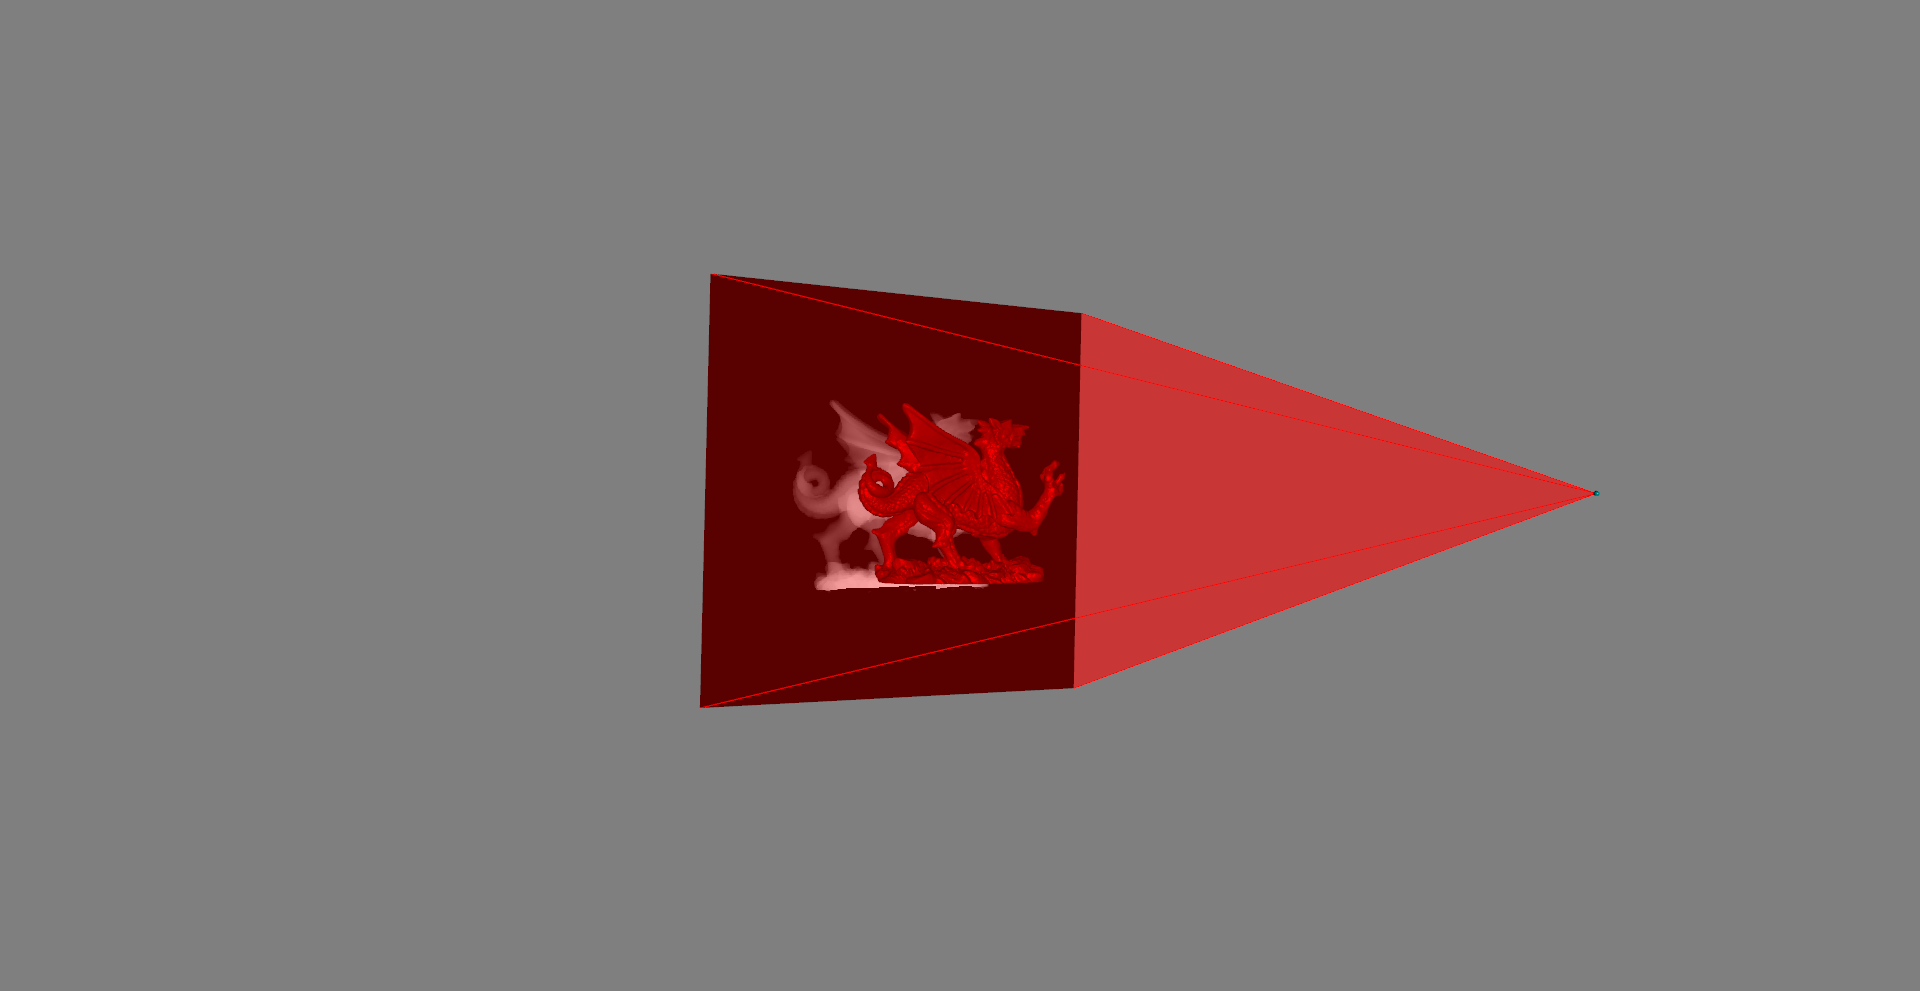
\includegraphics[width=0.25\textwidth]{beam_on.png}	&	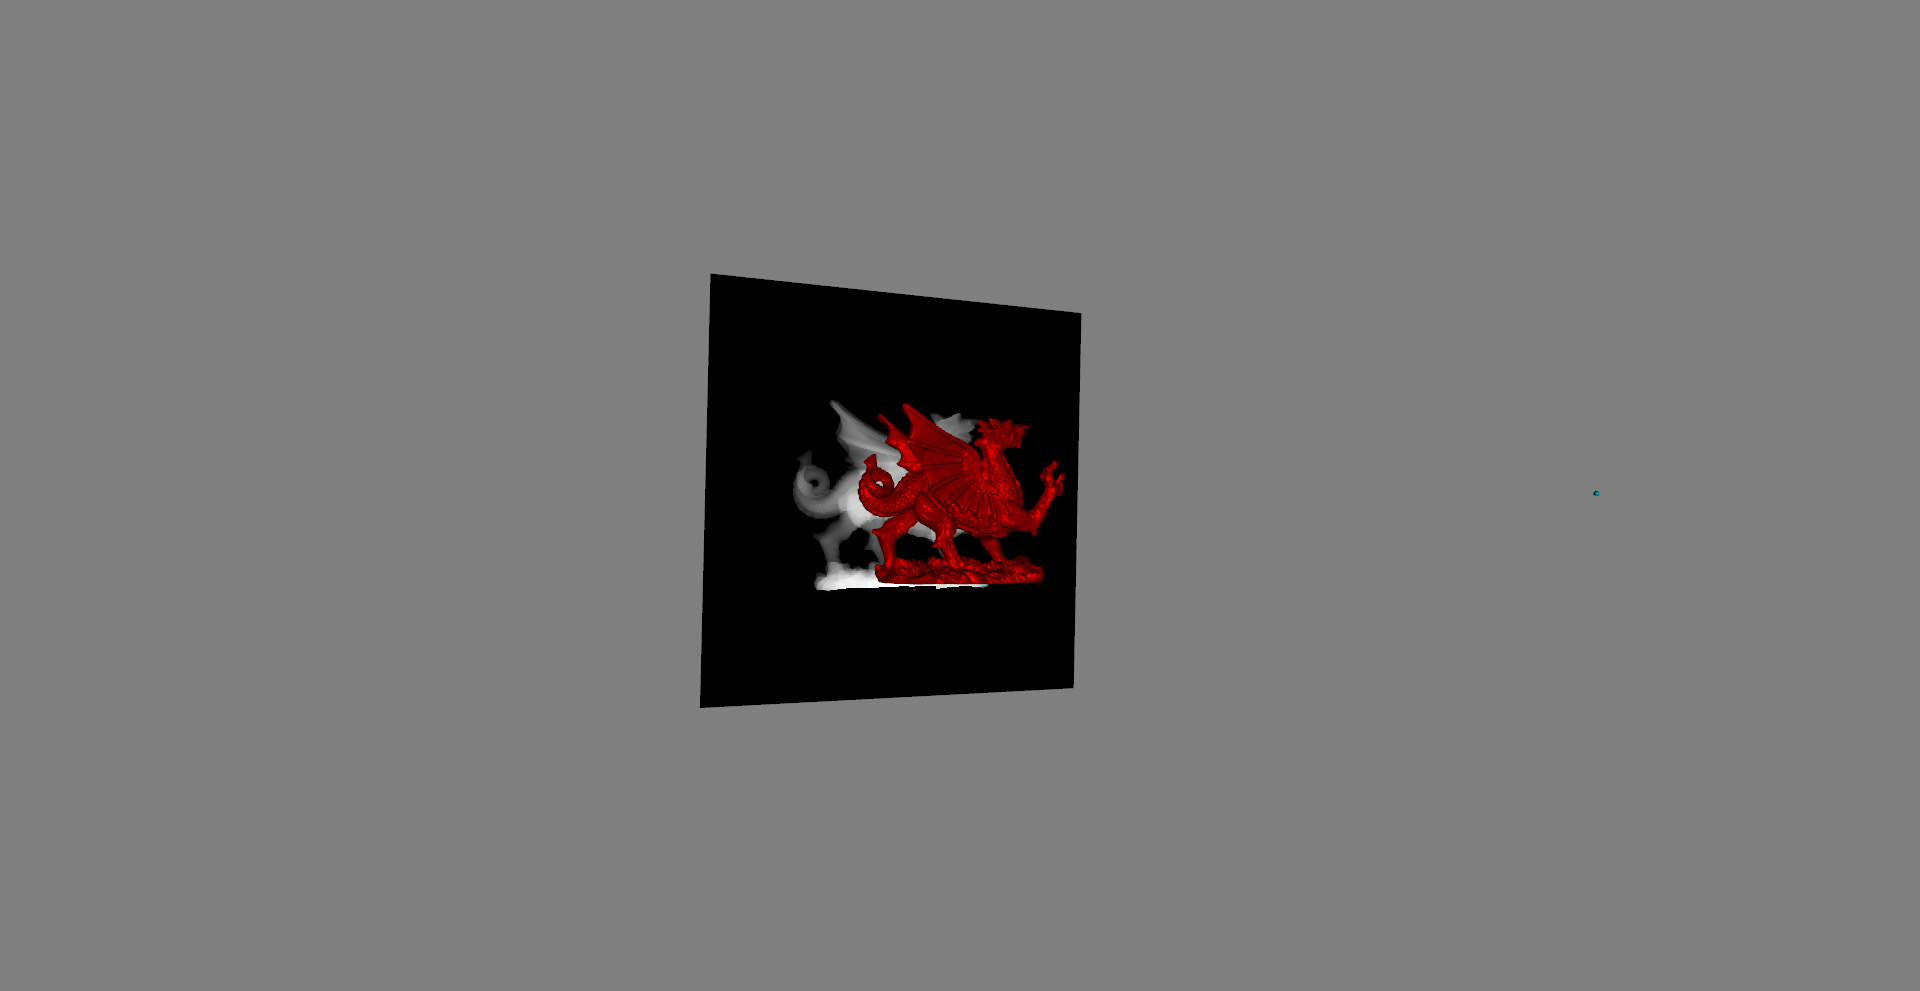
\includegraphics[width=0.25\textwidth]{beam_off.png}	&	Display the X-ray beam (on/off)\\
% 		\hline
% 		Key: \texttt{n}	&	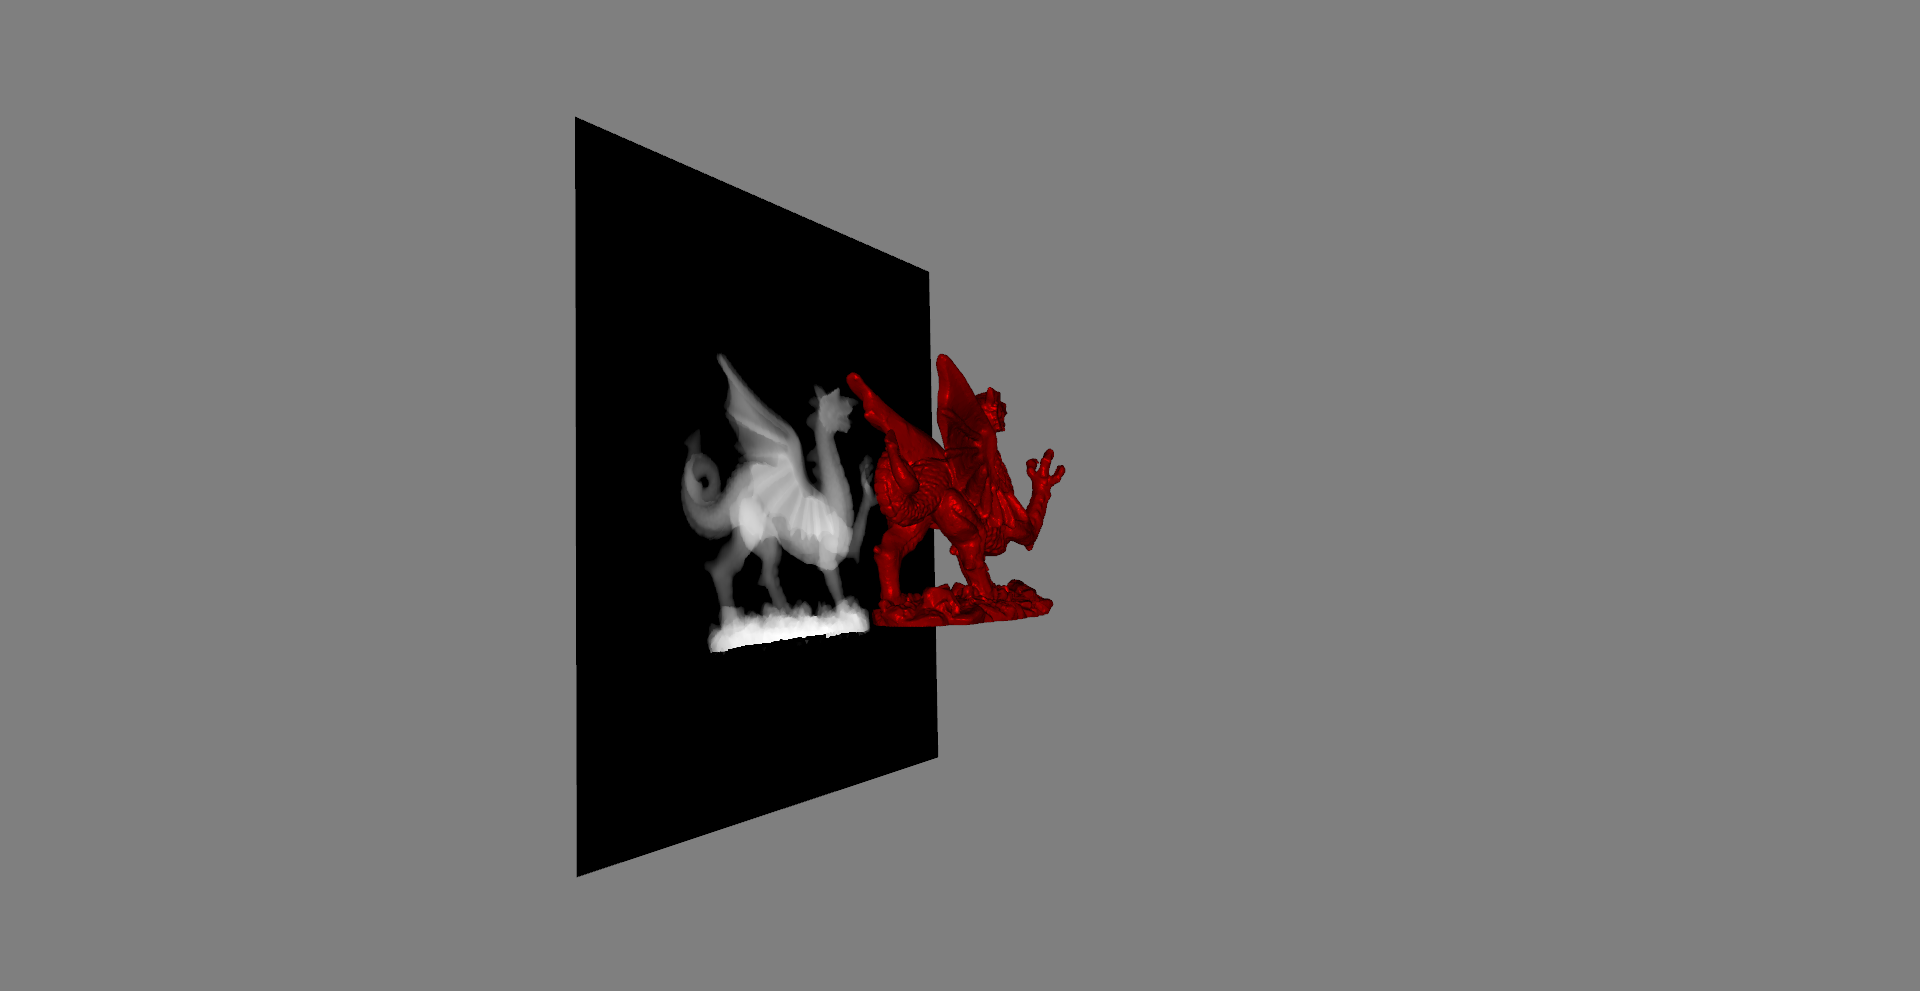
\includegraphics[width=0.25\textwidth]{negative_on.png}	&	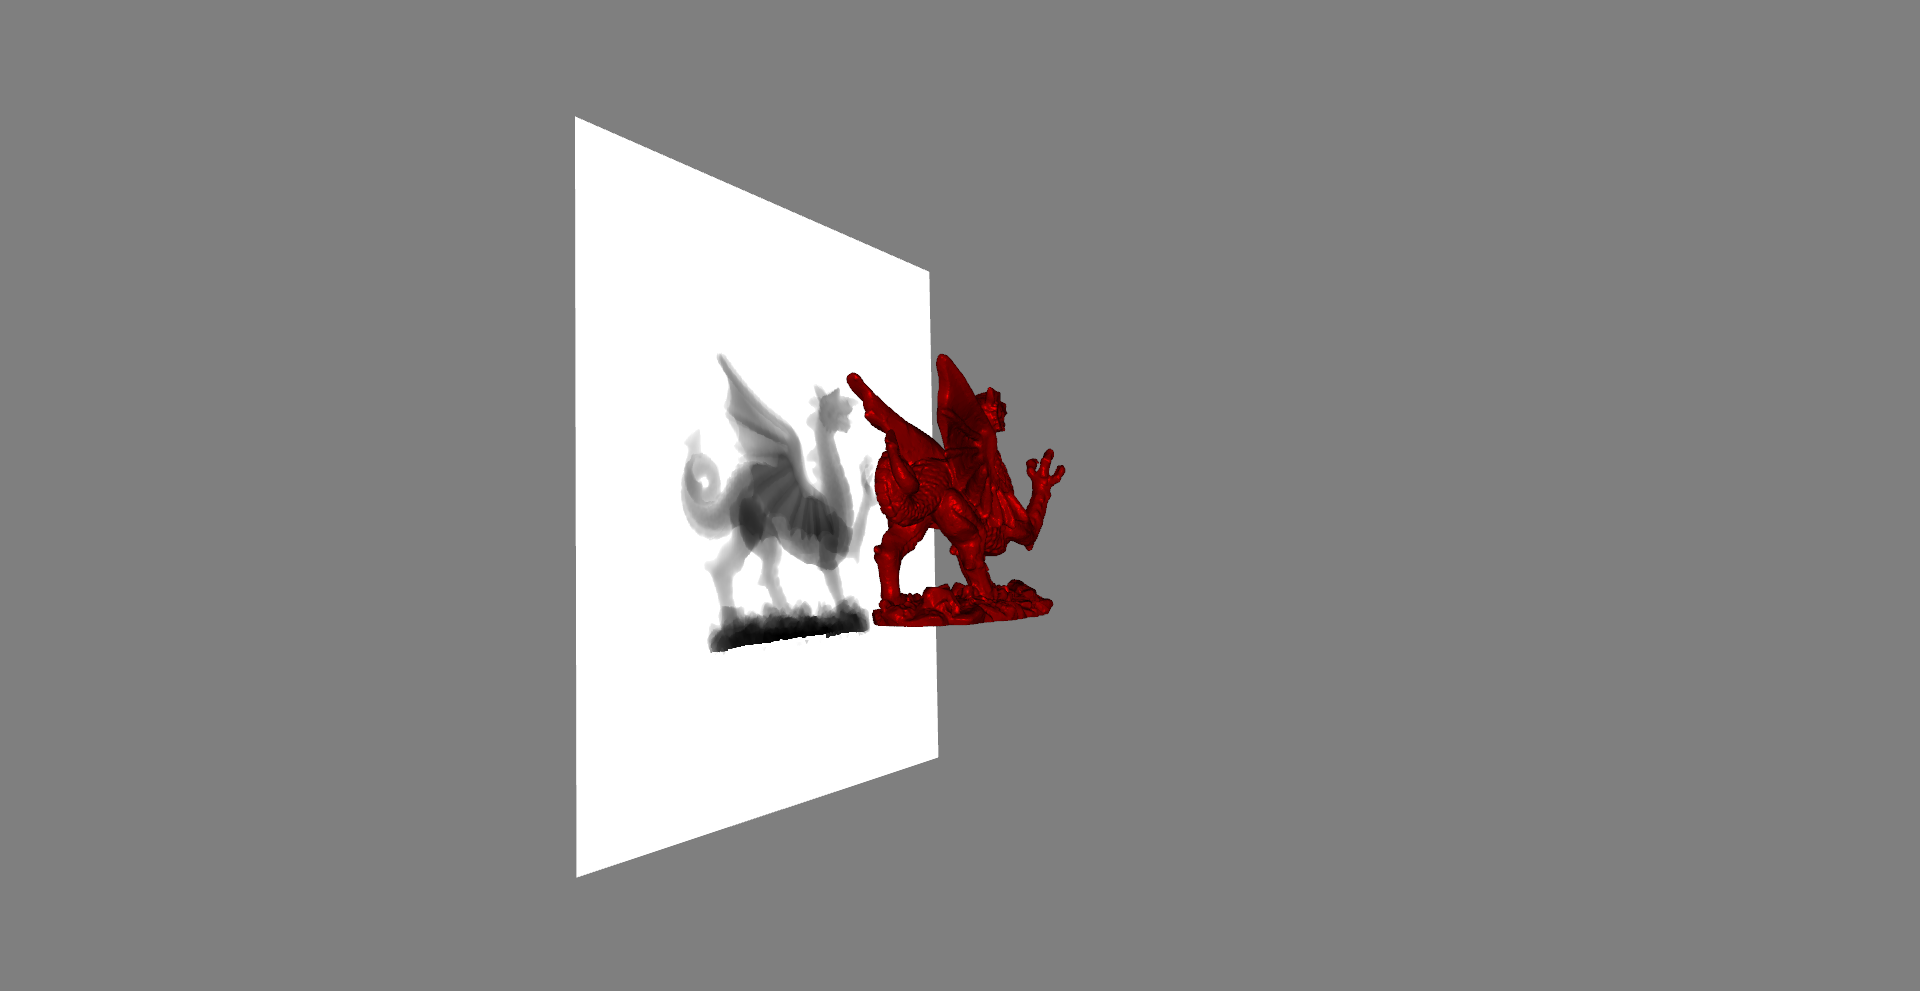
\includegraphics[width=0.25\textwidth]{negative_off.png}	&	Display the X-ray in negative (on/off)\\
% 		\hline
% 		Key: \texttt{s}	&	&	&	Stereo (on/off)\\
% 		\hline
% 		Key: \texttt{1}	&	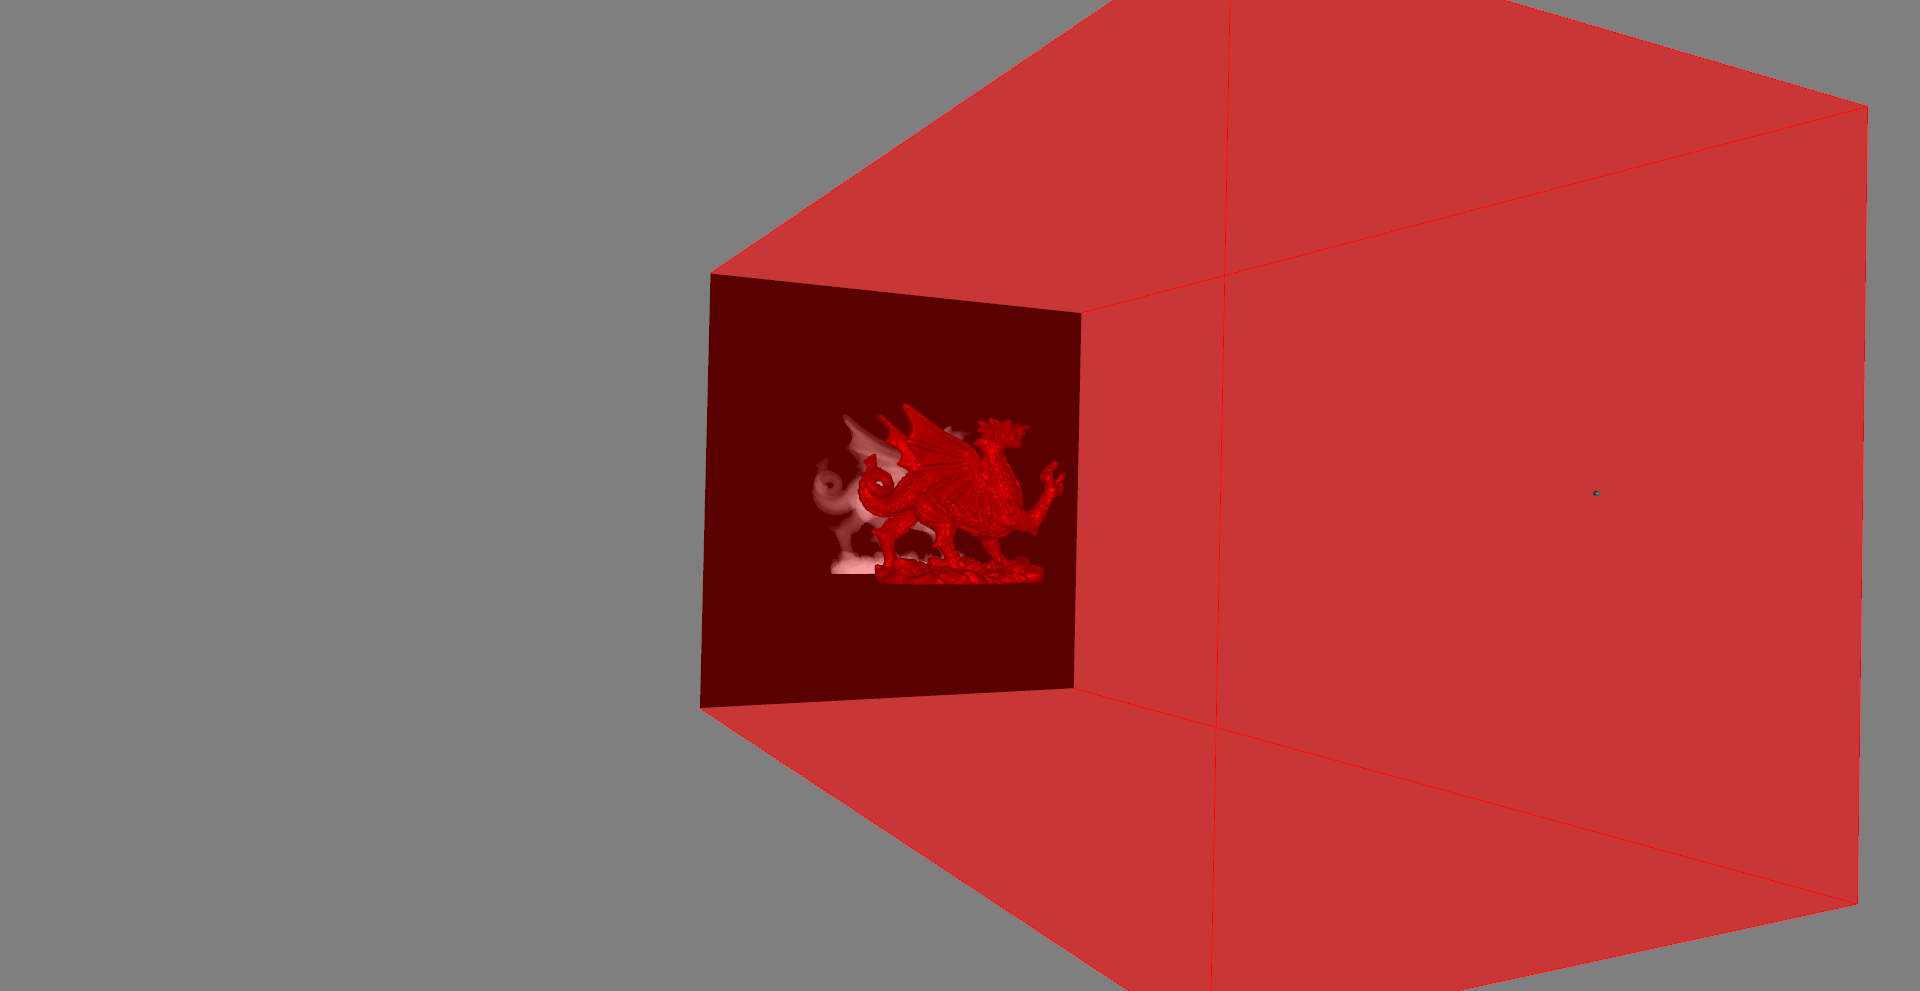
\includegraphics[width=0.25\textwidth]{parallel_beam.png}	&	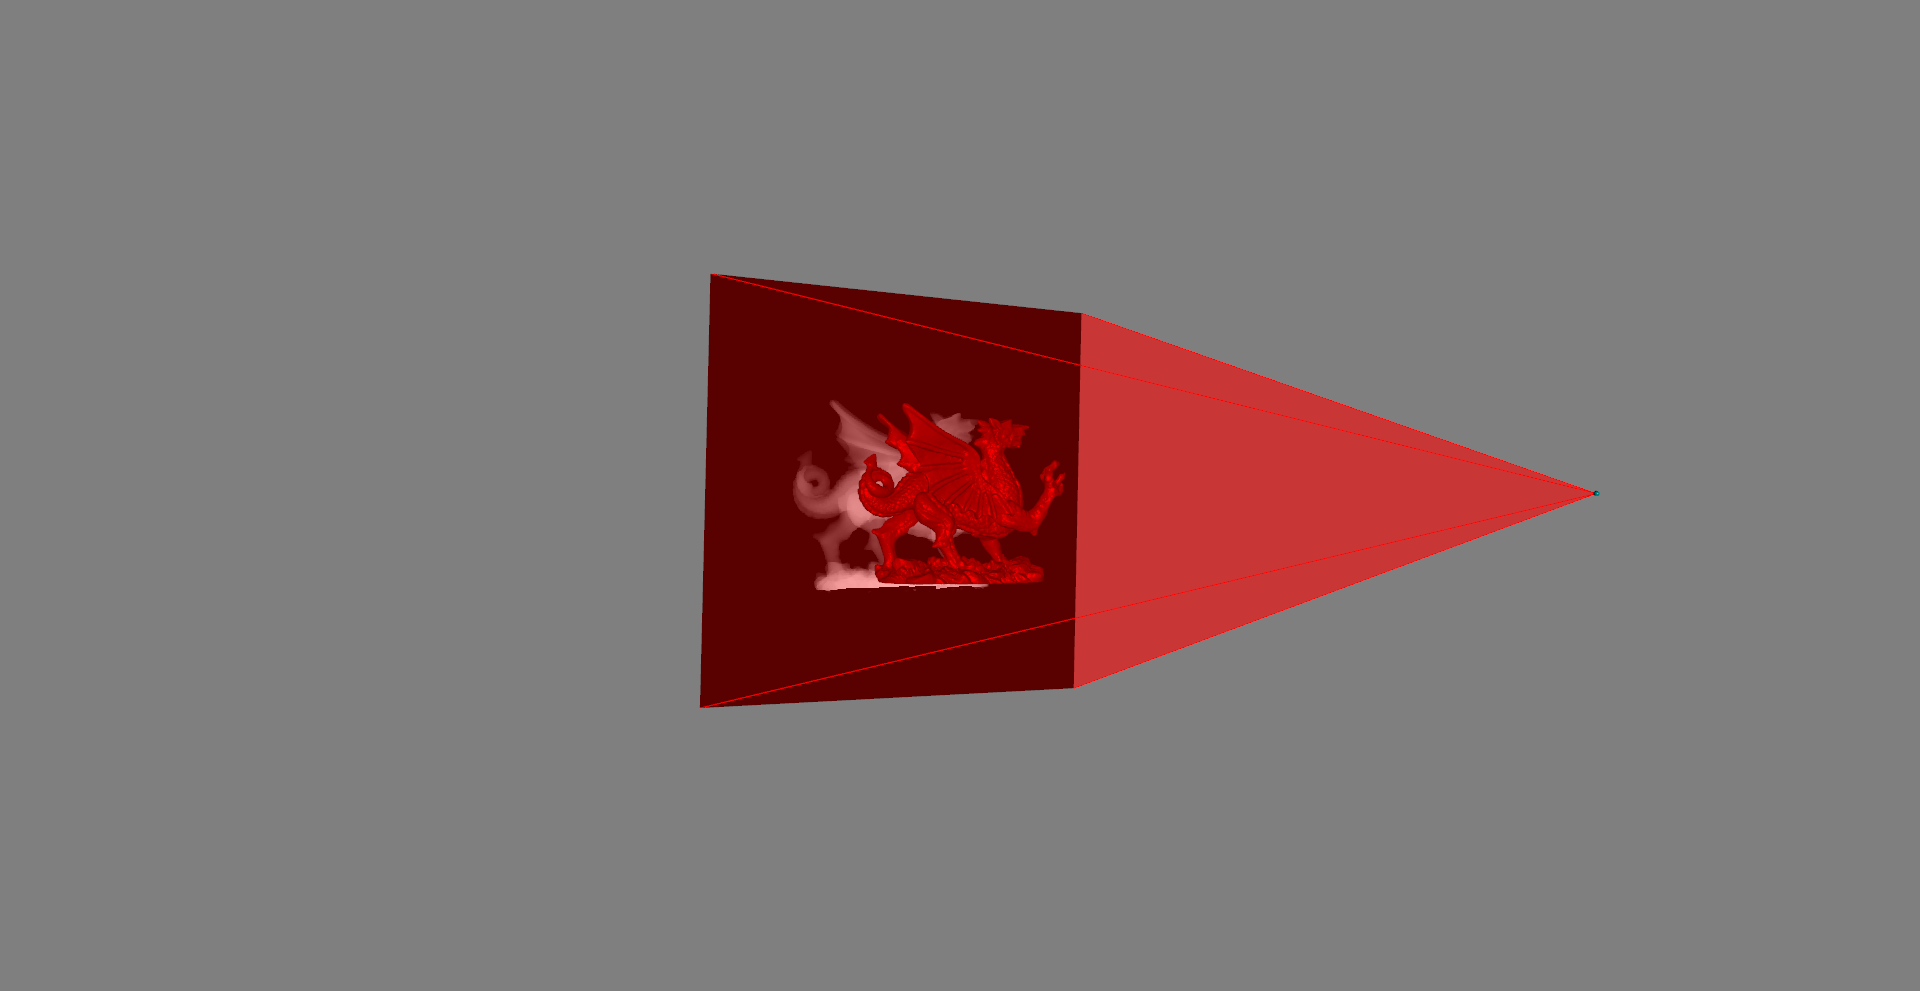
\includegraphics[width=0.25\textwidth]{point_source.png}	&	Use a parallel beam/Use a point source\\
% 		\hline
% 		Key: \texttt{2}	&	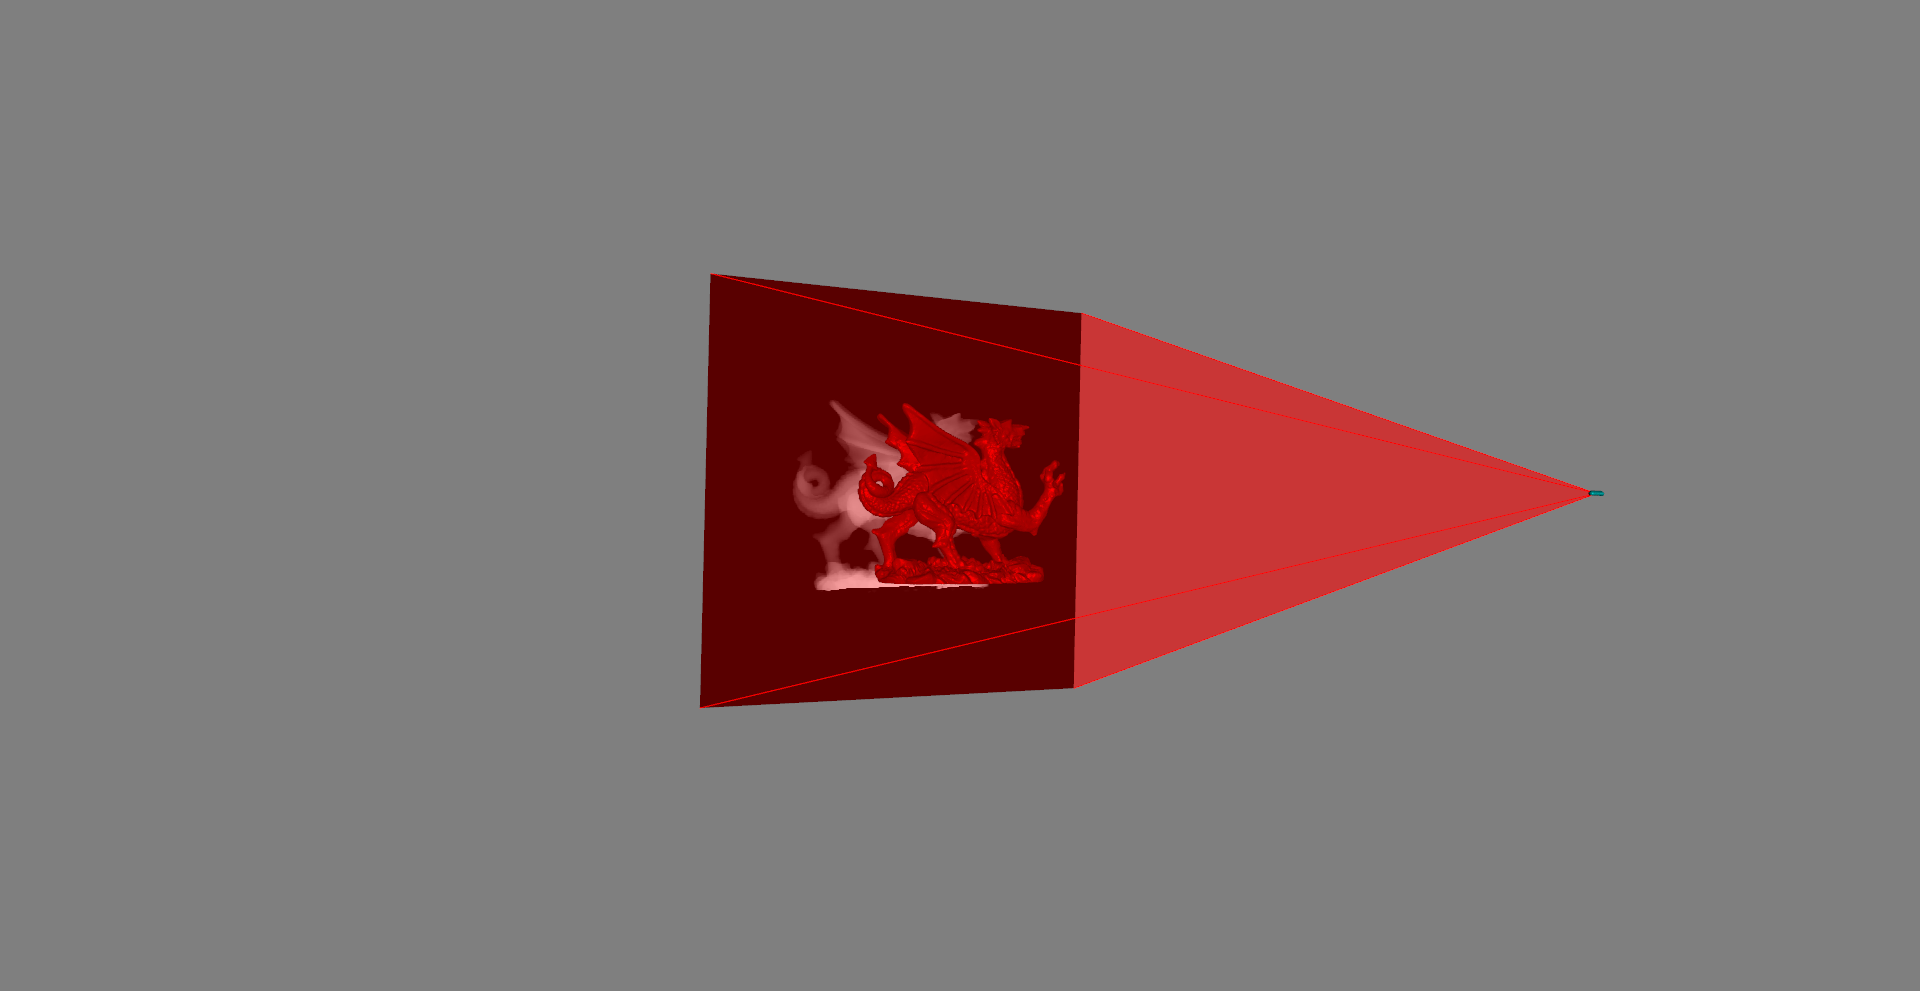
\includegraphics[width=0.25\textwidth]{line_source.png}	&	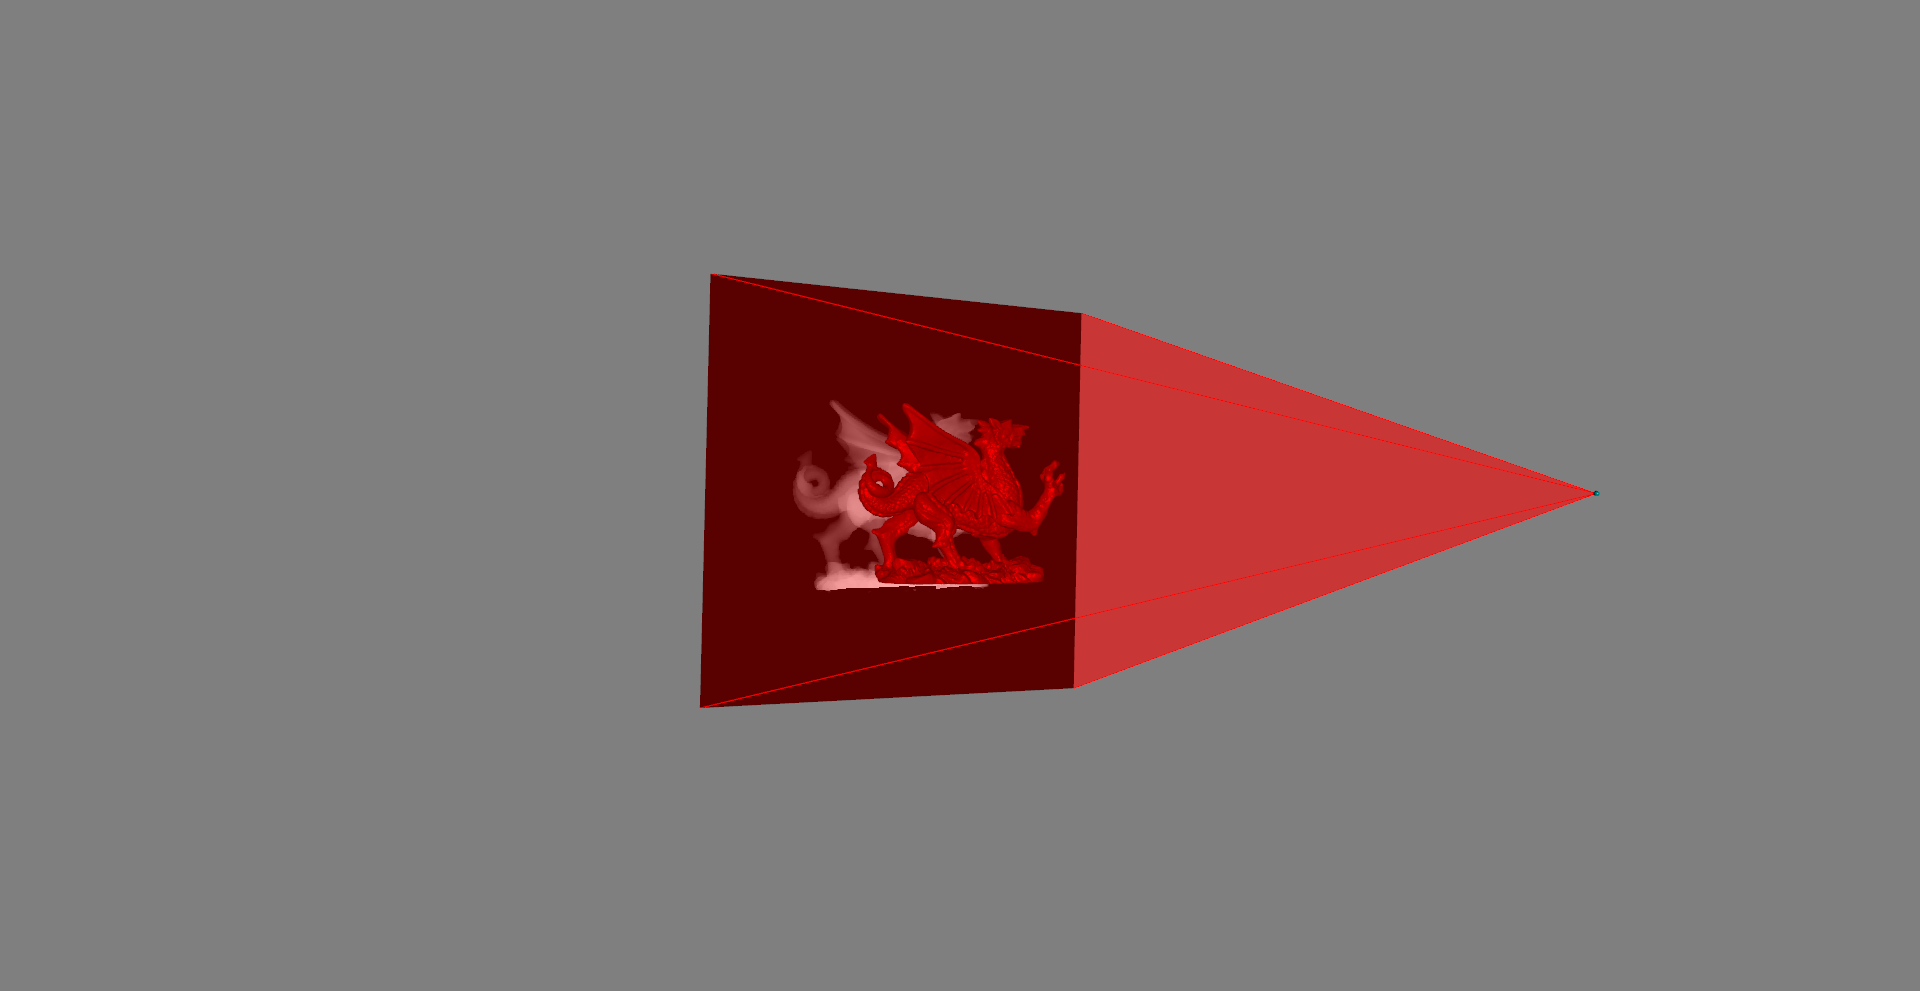
\includegraphics[width=0.25\textwidth]{point_source.png}	&	Use a line source/Use a point source\\
% 		\hline
% 		Key: \texttt{3}	&	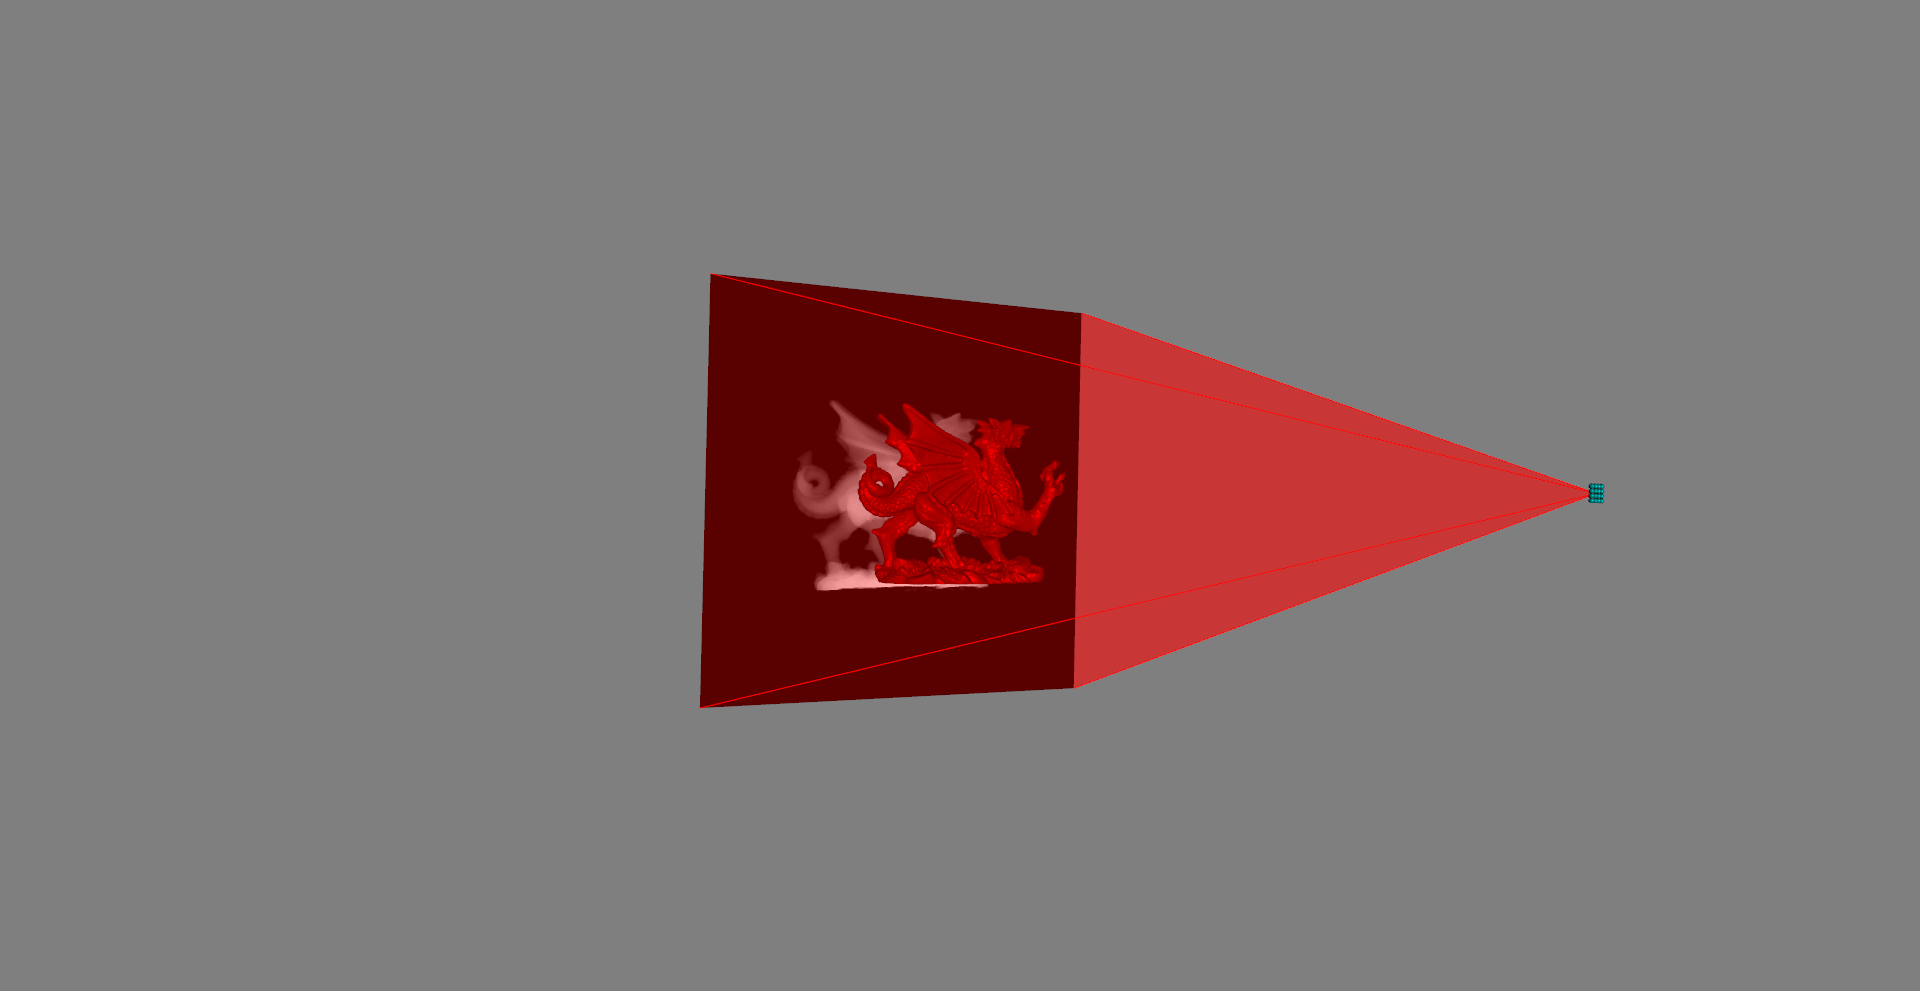
\includegraphics[width=0.25\textwidth]{square_source.png}	&	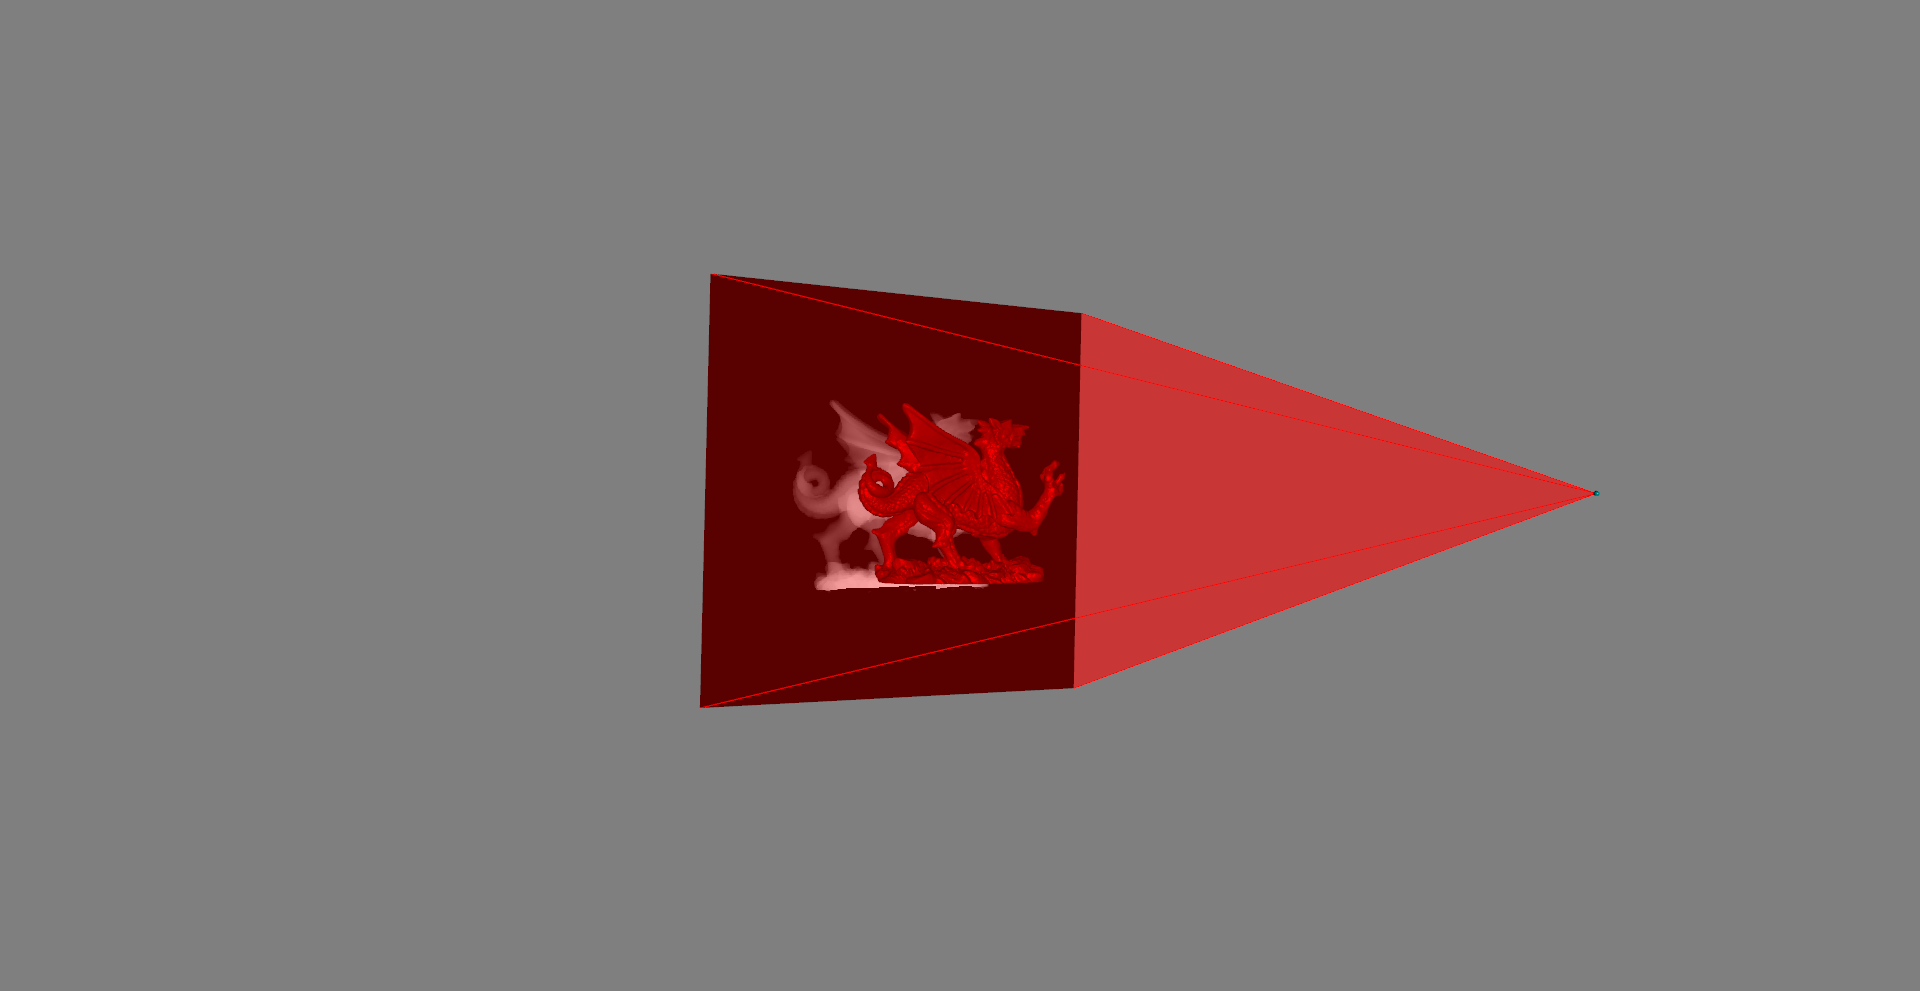
\includegraphics[width=0.25\textwidth]{point_source.png}	&	Use a square source/Use a point source\\
% 		\hline
% 		Key: \texttt{4}	&	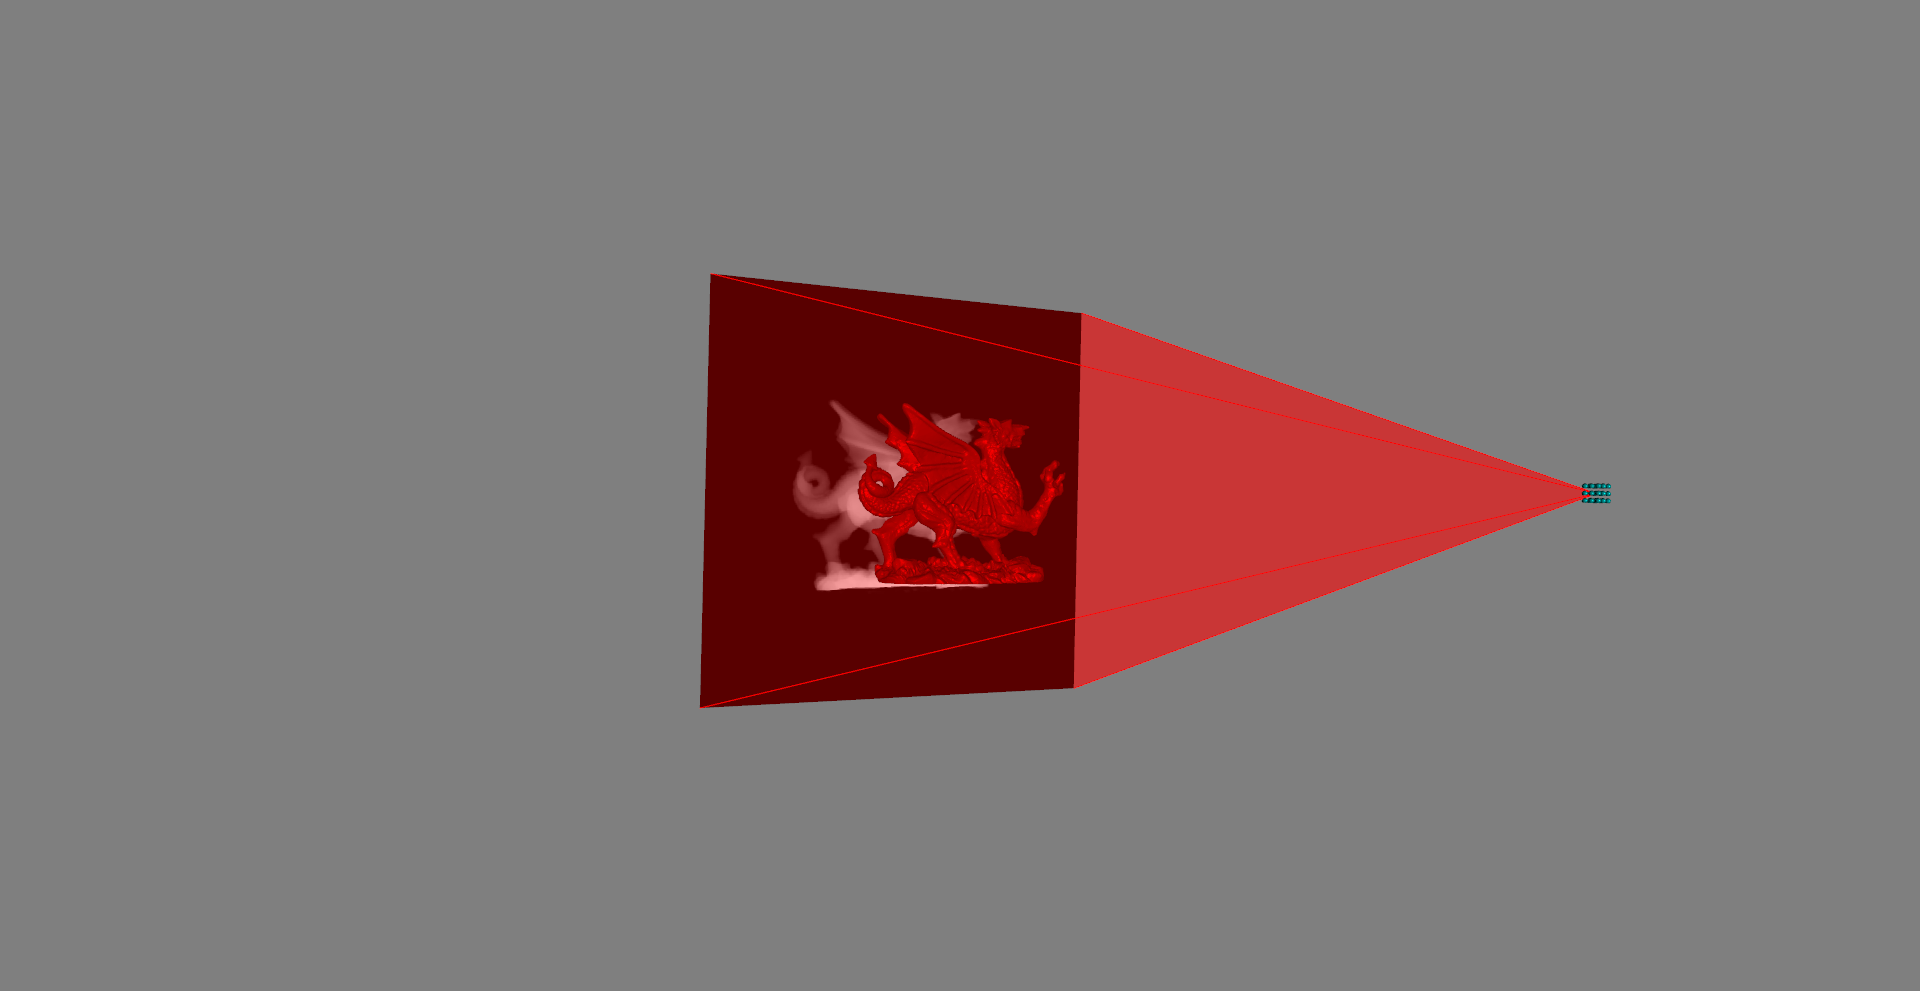
\includegraphics[width=0.25\textwidth]{cube_source.png}	&	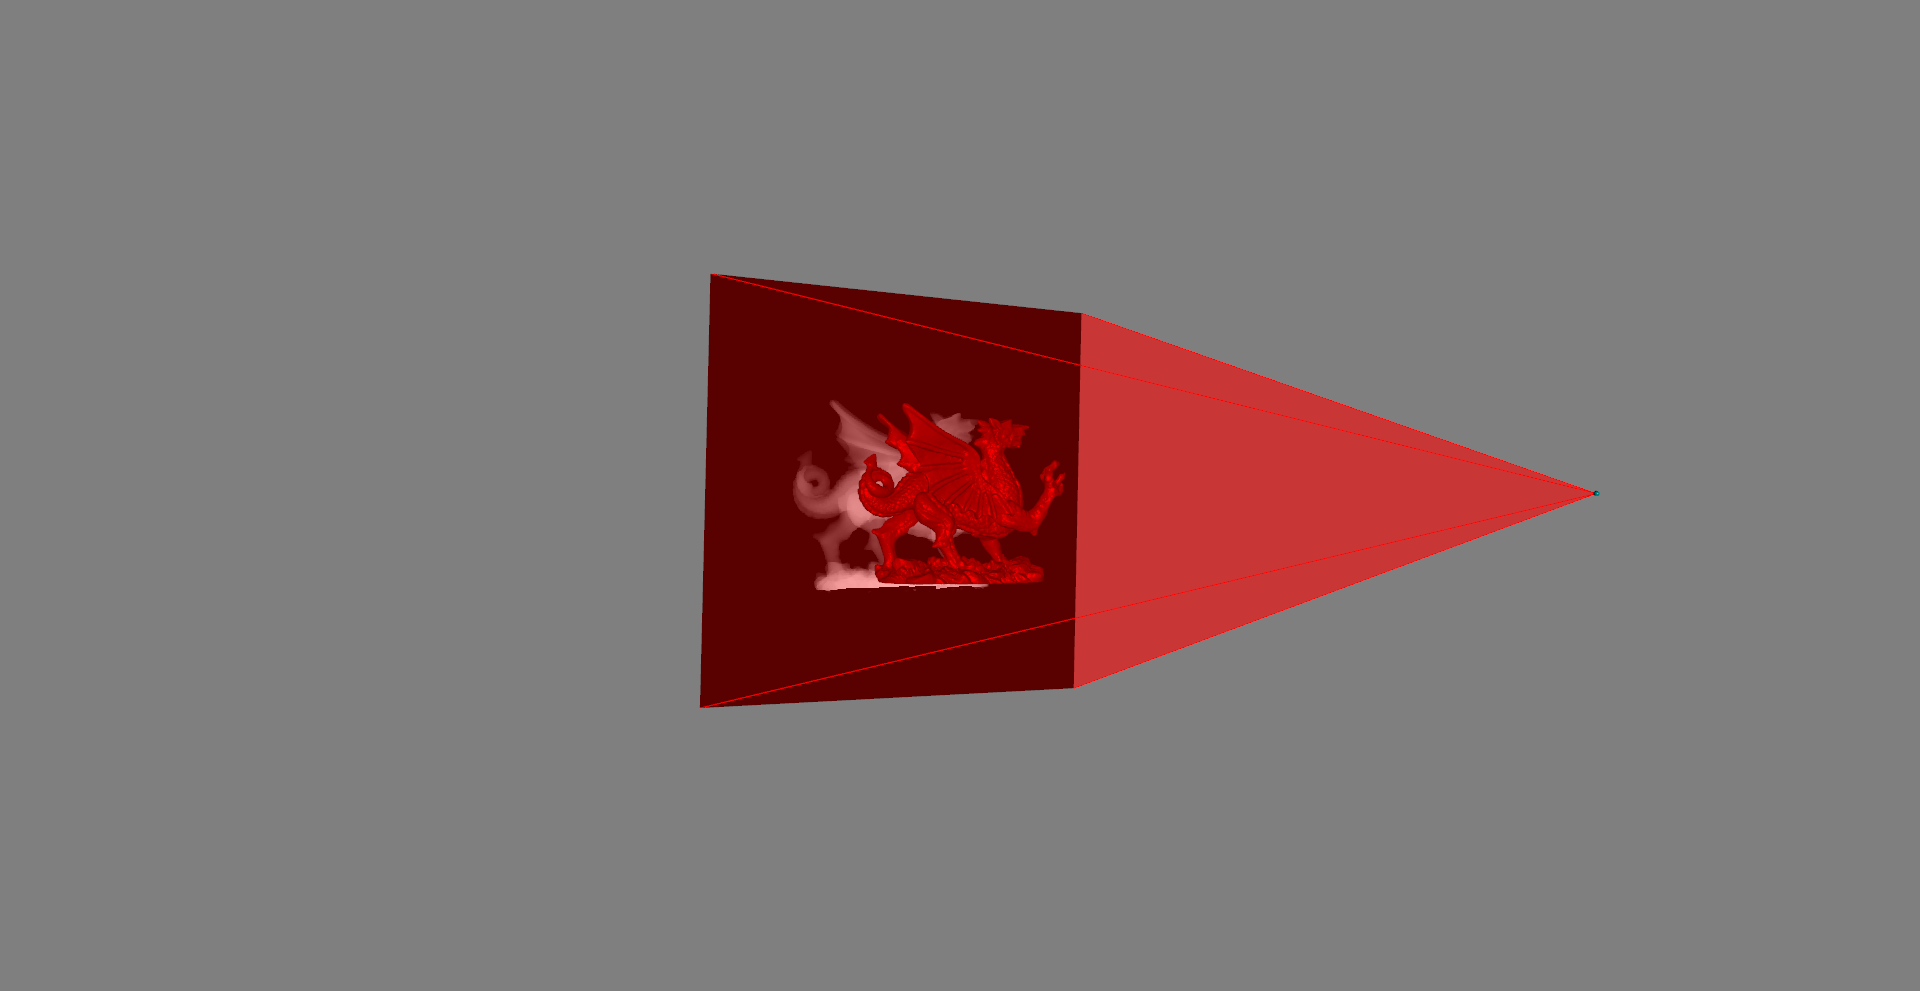
\includegraphics[width=0.25\textwidth]{point_source.png}	&	Use a cube source/Use a point source\\
% 		\hline
		Mouse wheel	&	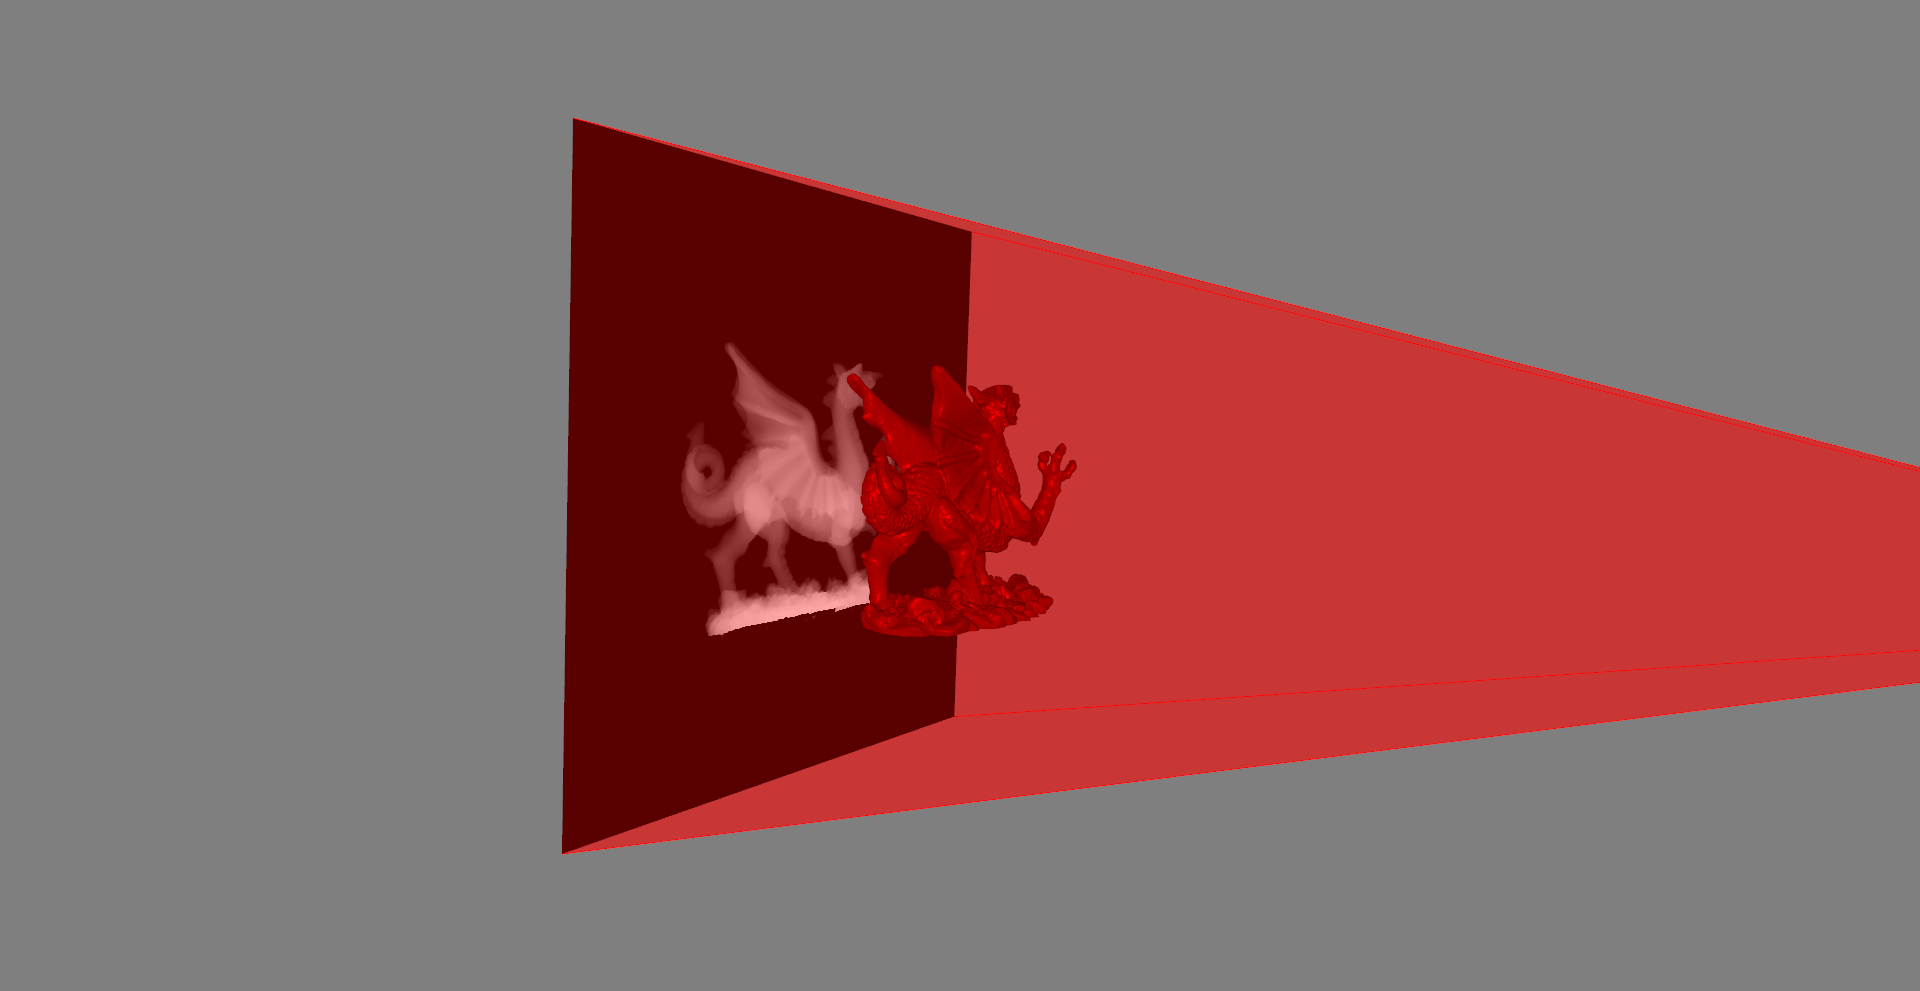
\includegraphics[width=0.25\textwidth]{mouse_wheel_zoom_in.png}	&	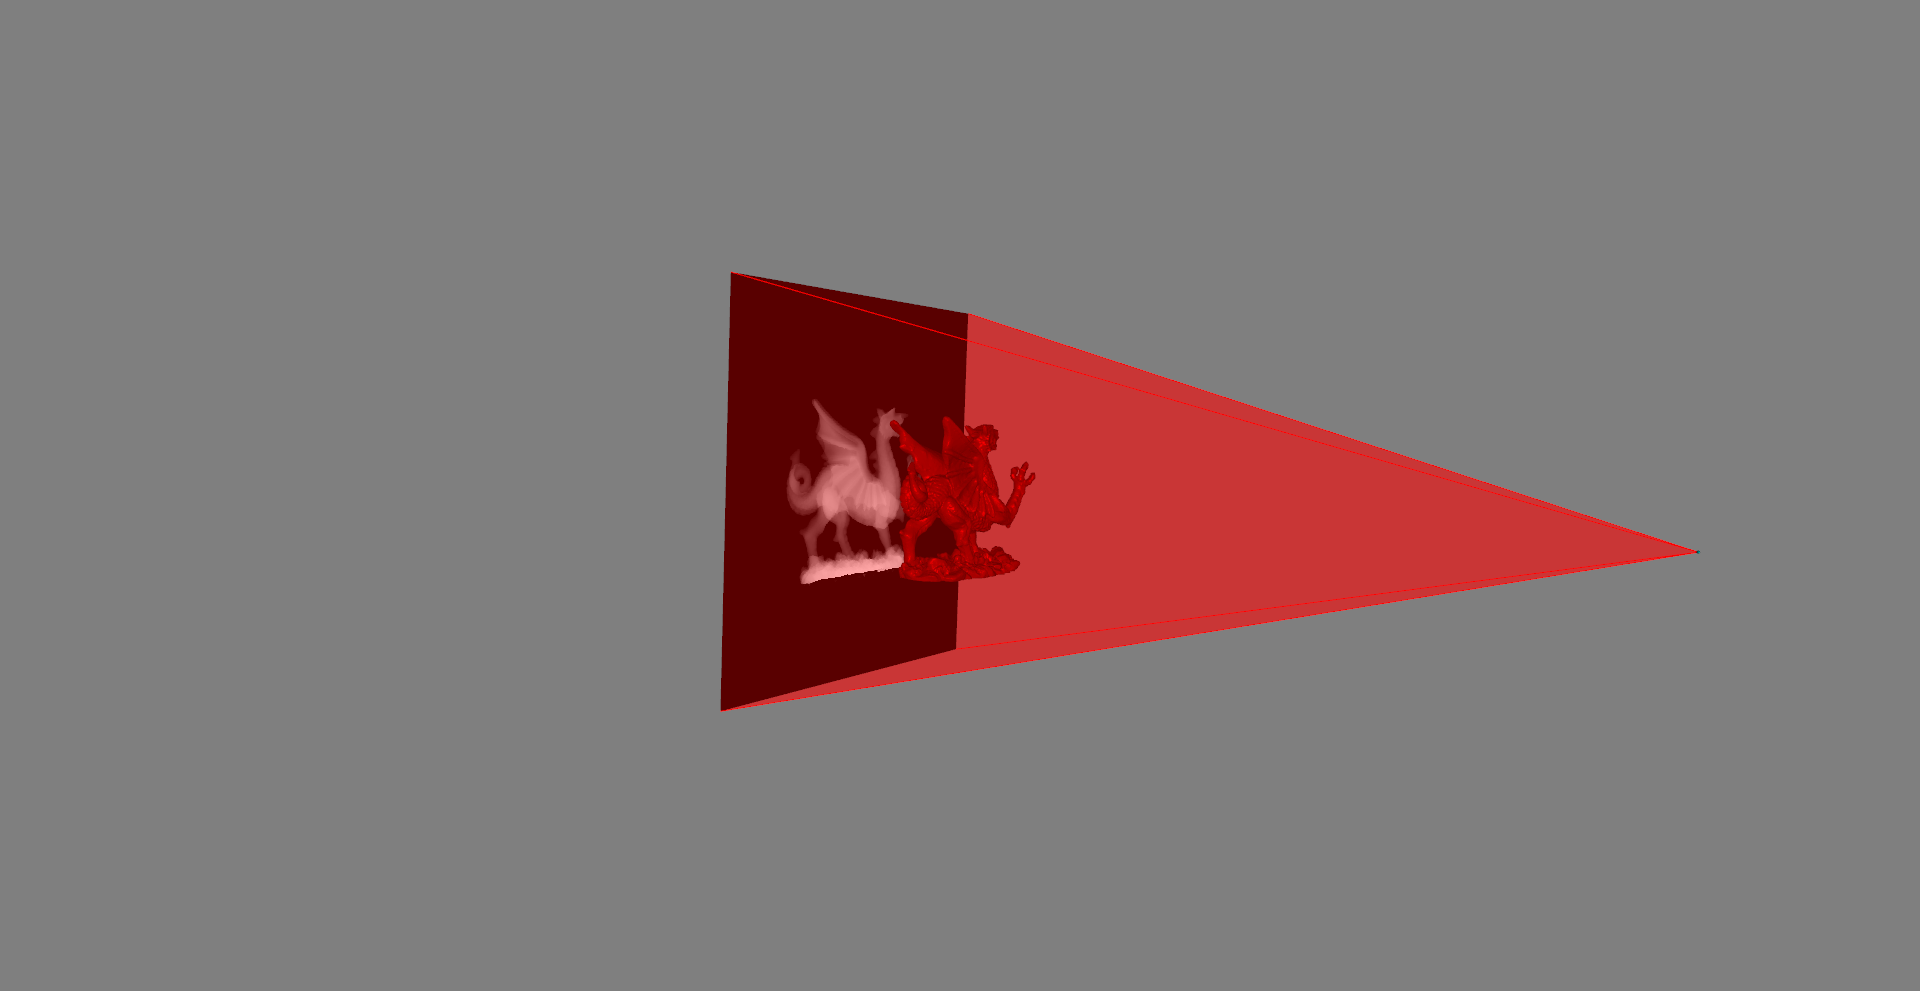
\includegraphics[width=0.25\textwidth]{mouse_wheel_zoom_out.png}	&	Zoom in/out\\
		\hline
		Mouse left button	&	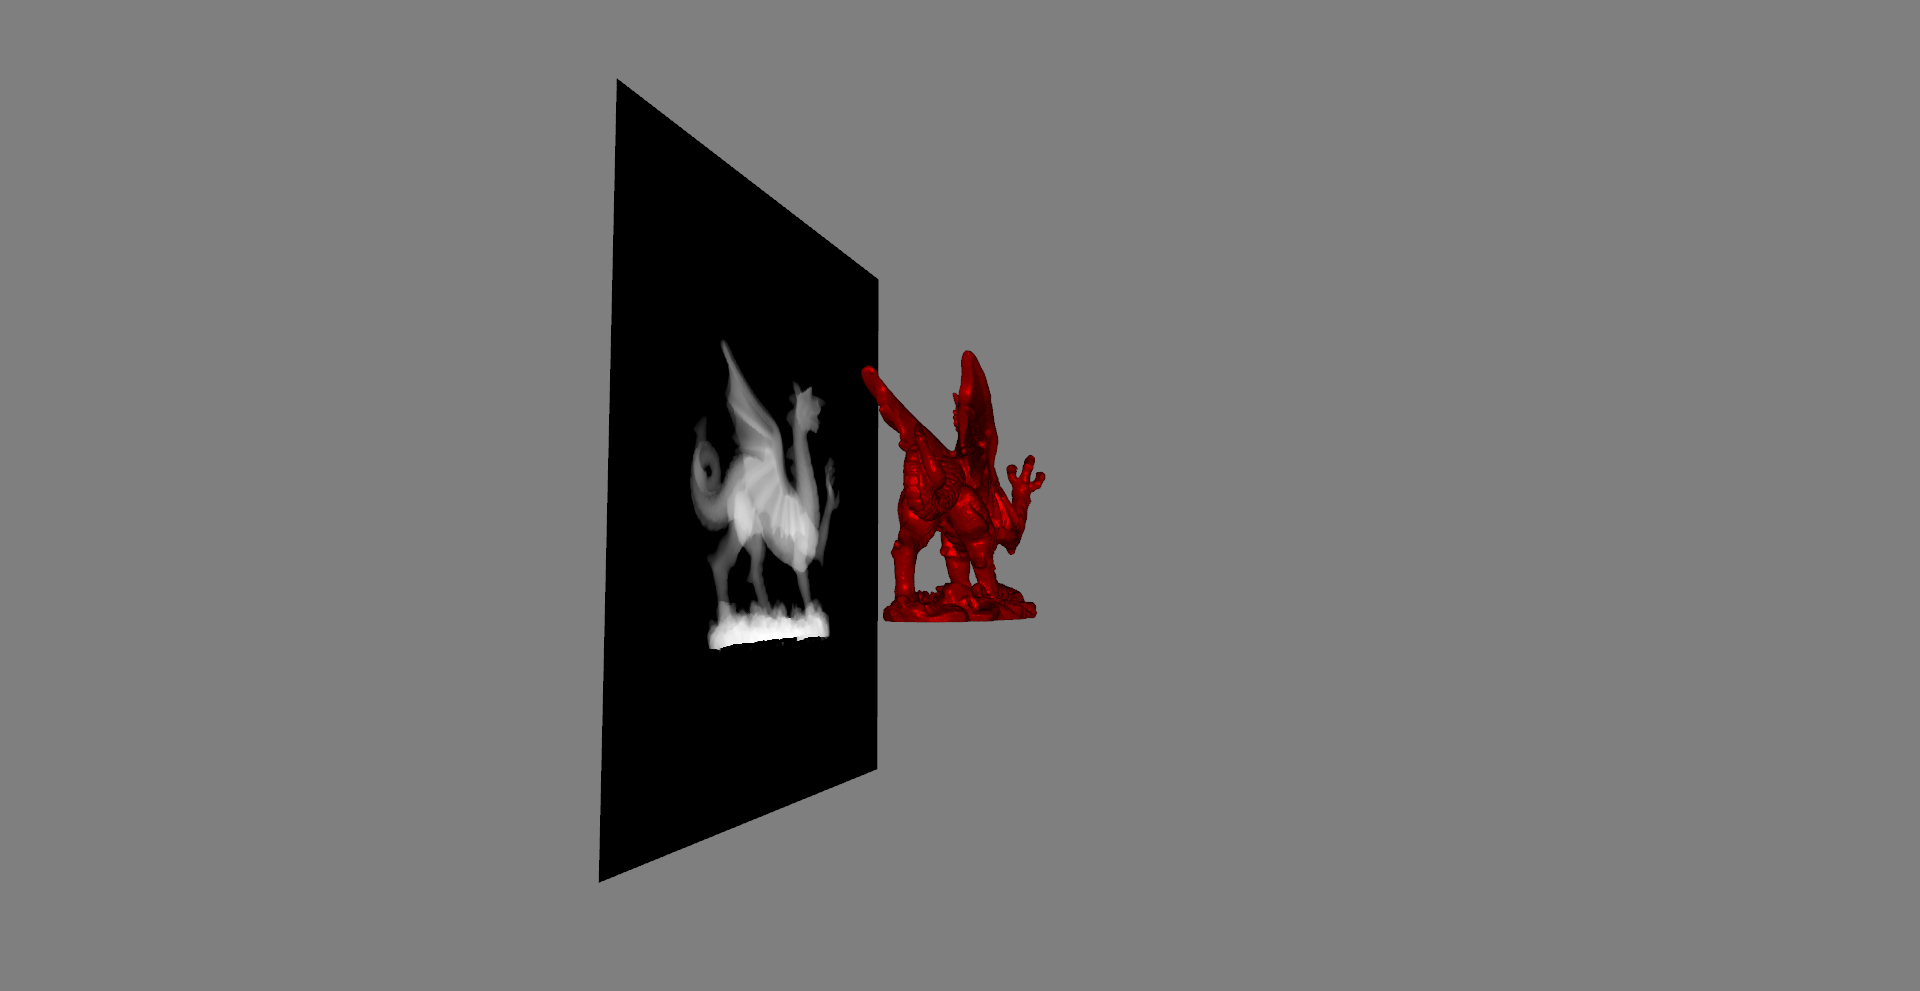
\includegraphics[width=0.25\textwidth]{mouse_click.png}	&	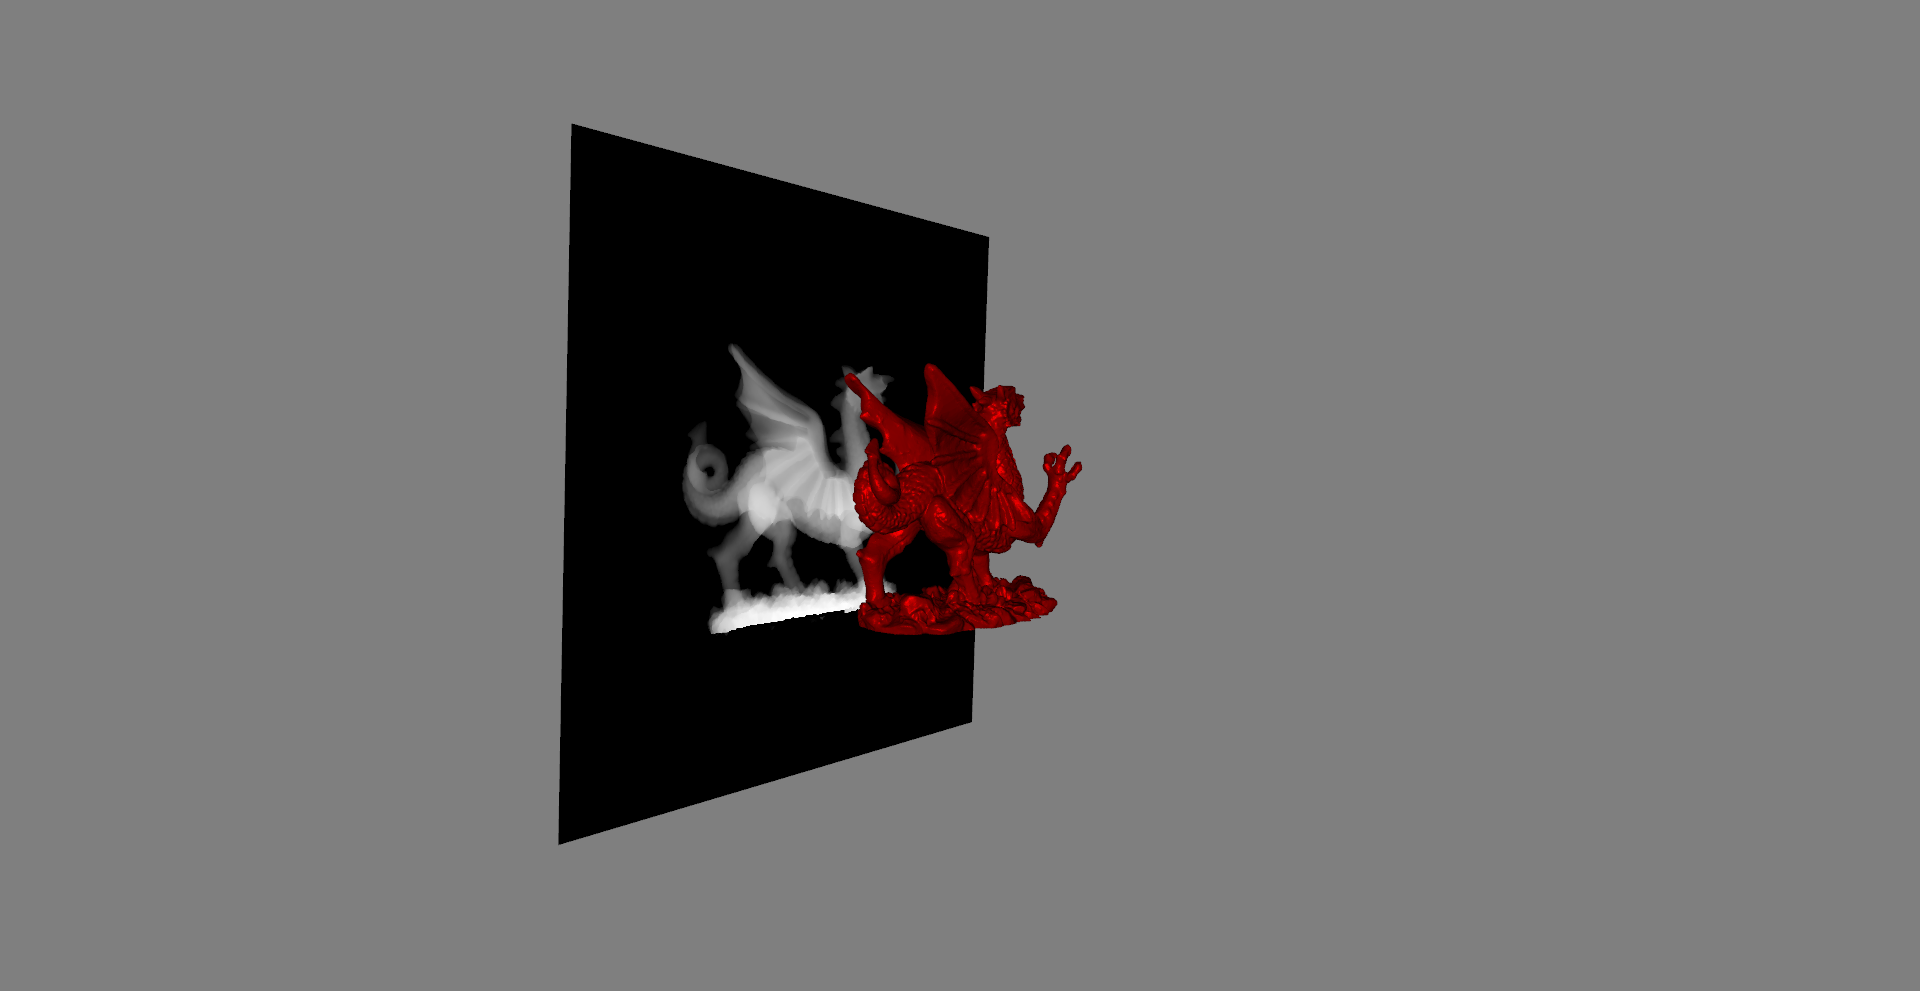
\includegraphics[width=0.25\textwidth]{mouse_left_click.png}	&	Rotate the virtual environment\\
		\hline
		Mouse middle button	&	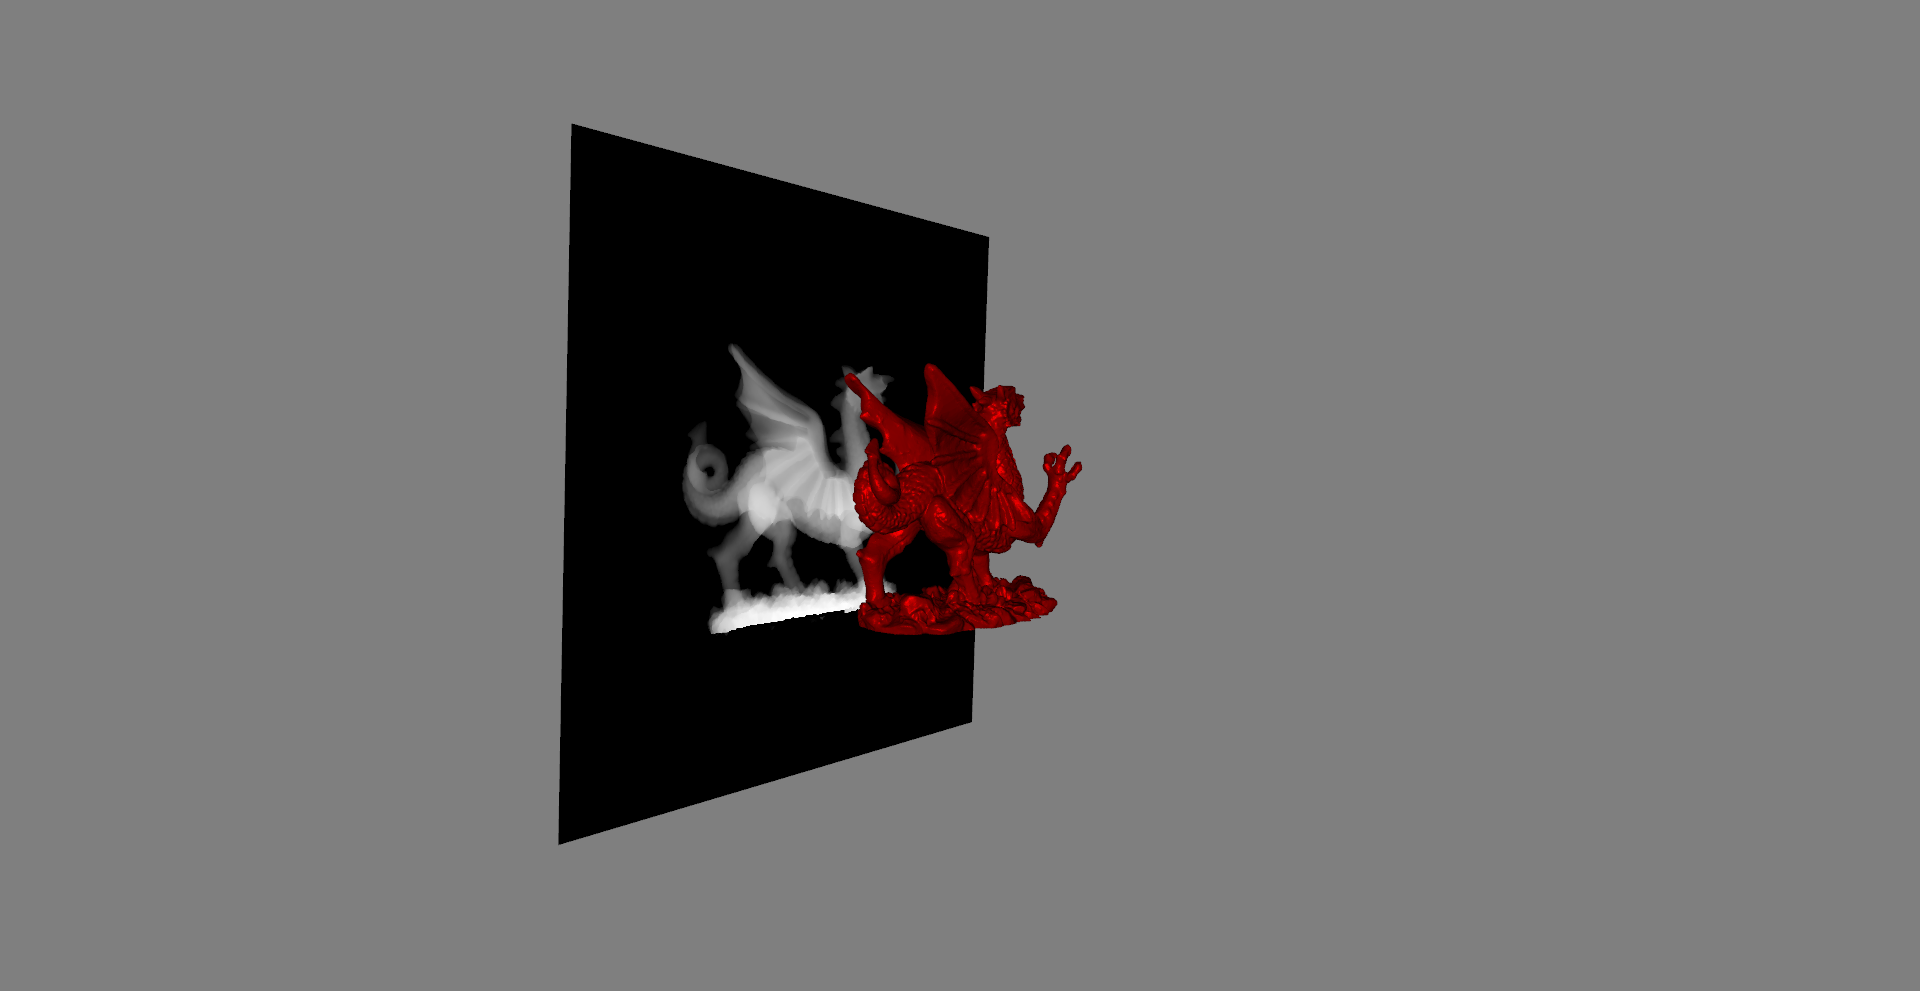
\includegraphics[width=0.25\textwidth]{mouse_left_click.png}	&	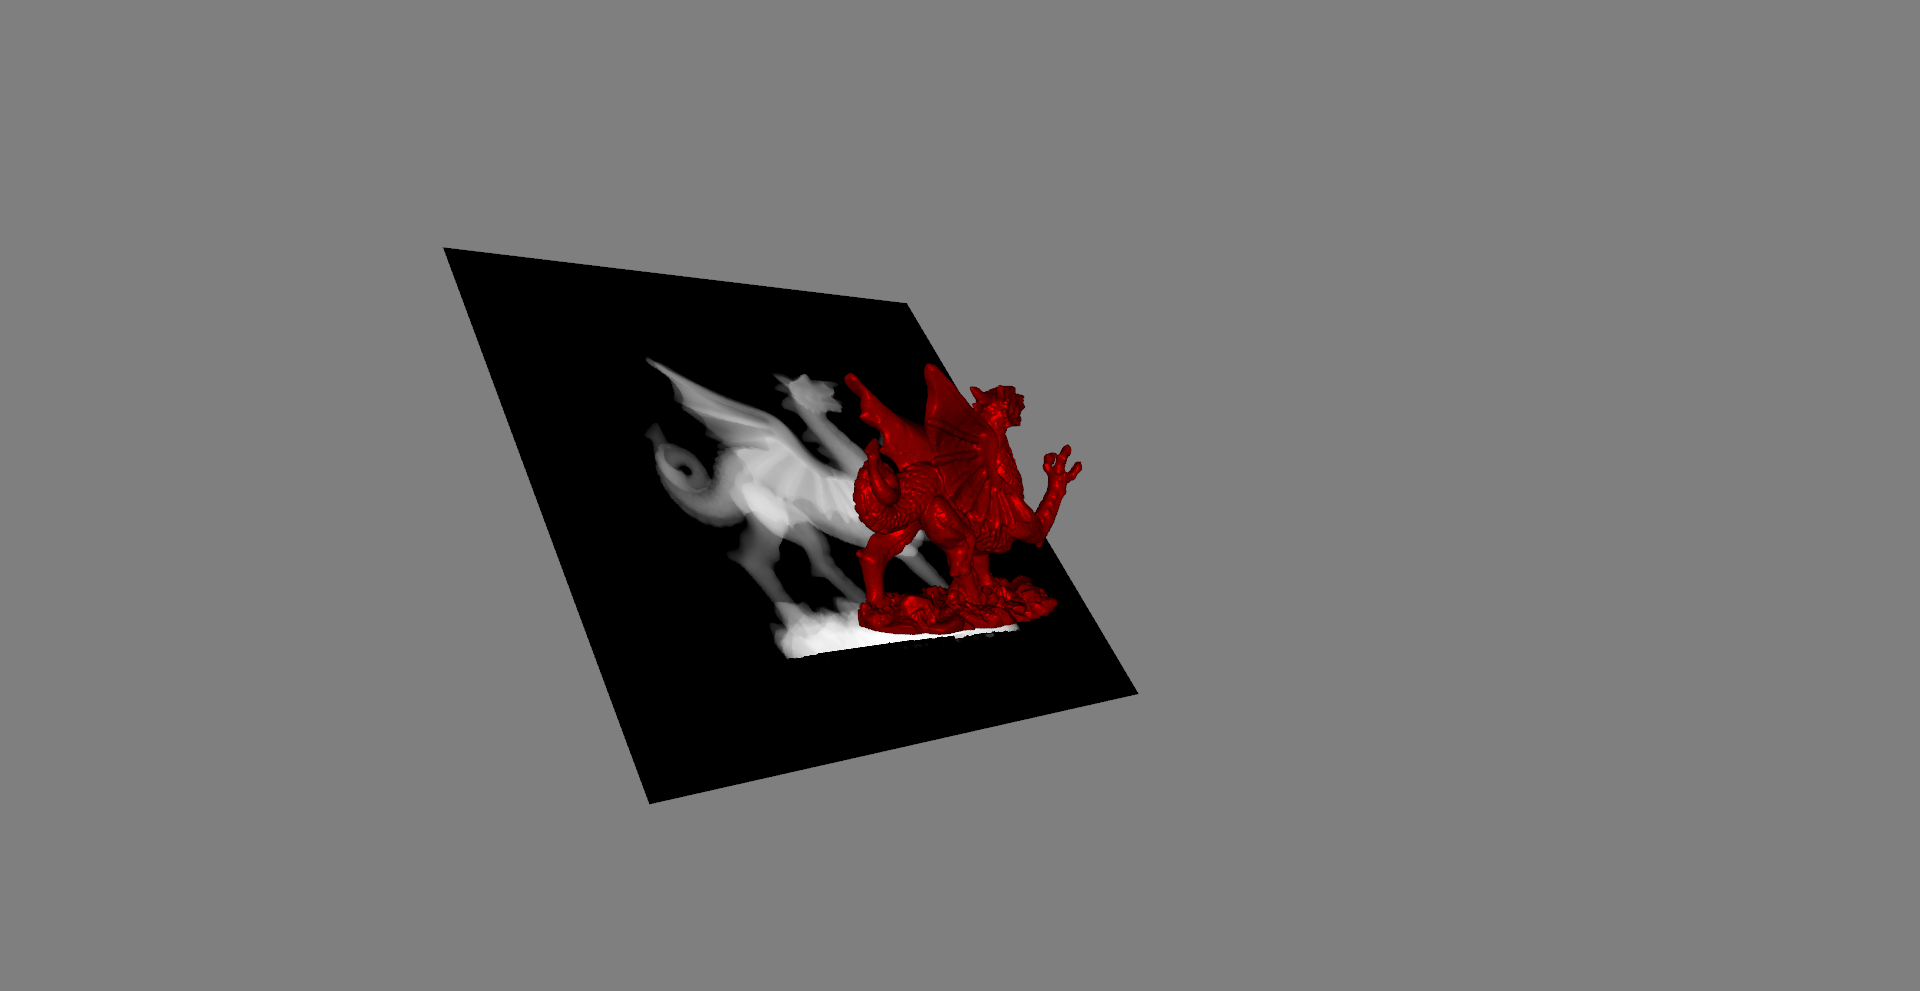
\includegraphics[width=0.25\textwidth]{mouse_middle_click.png}	&	Rotate the X-ray detector\\
		\hline
		Mouse right button	&	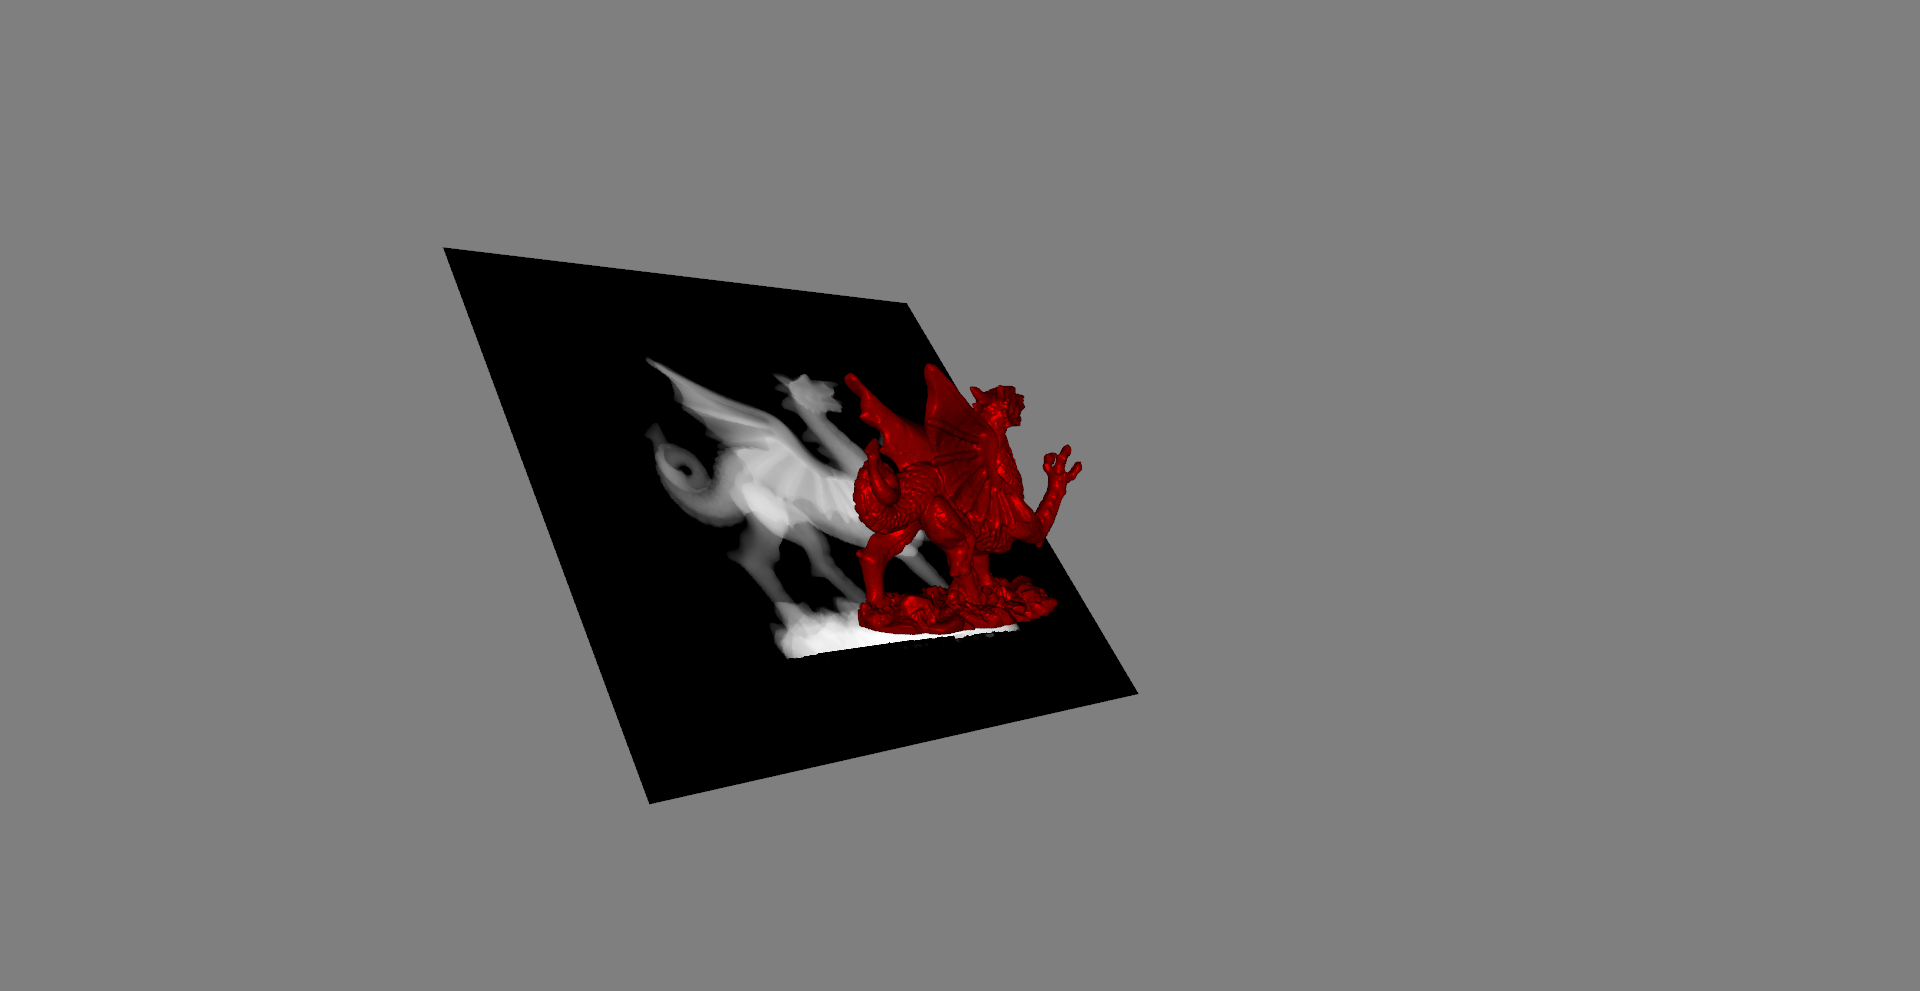
\includegraphics[width=0.25\textwidth]{mouse_middle_click.png}	&	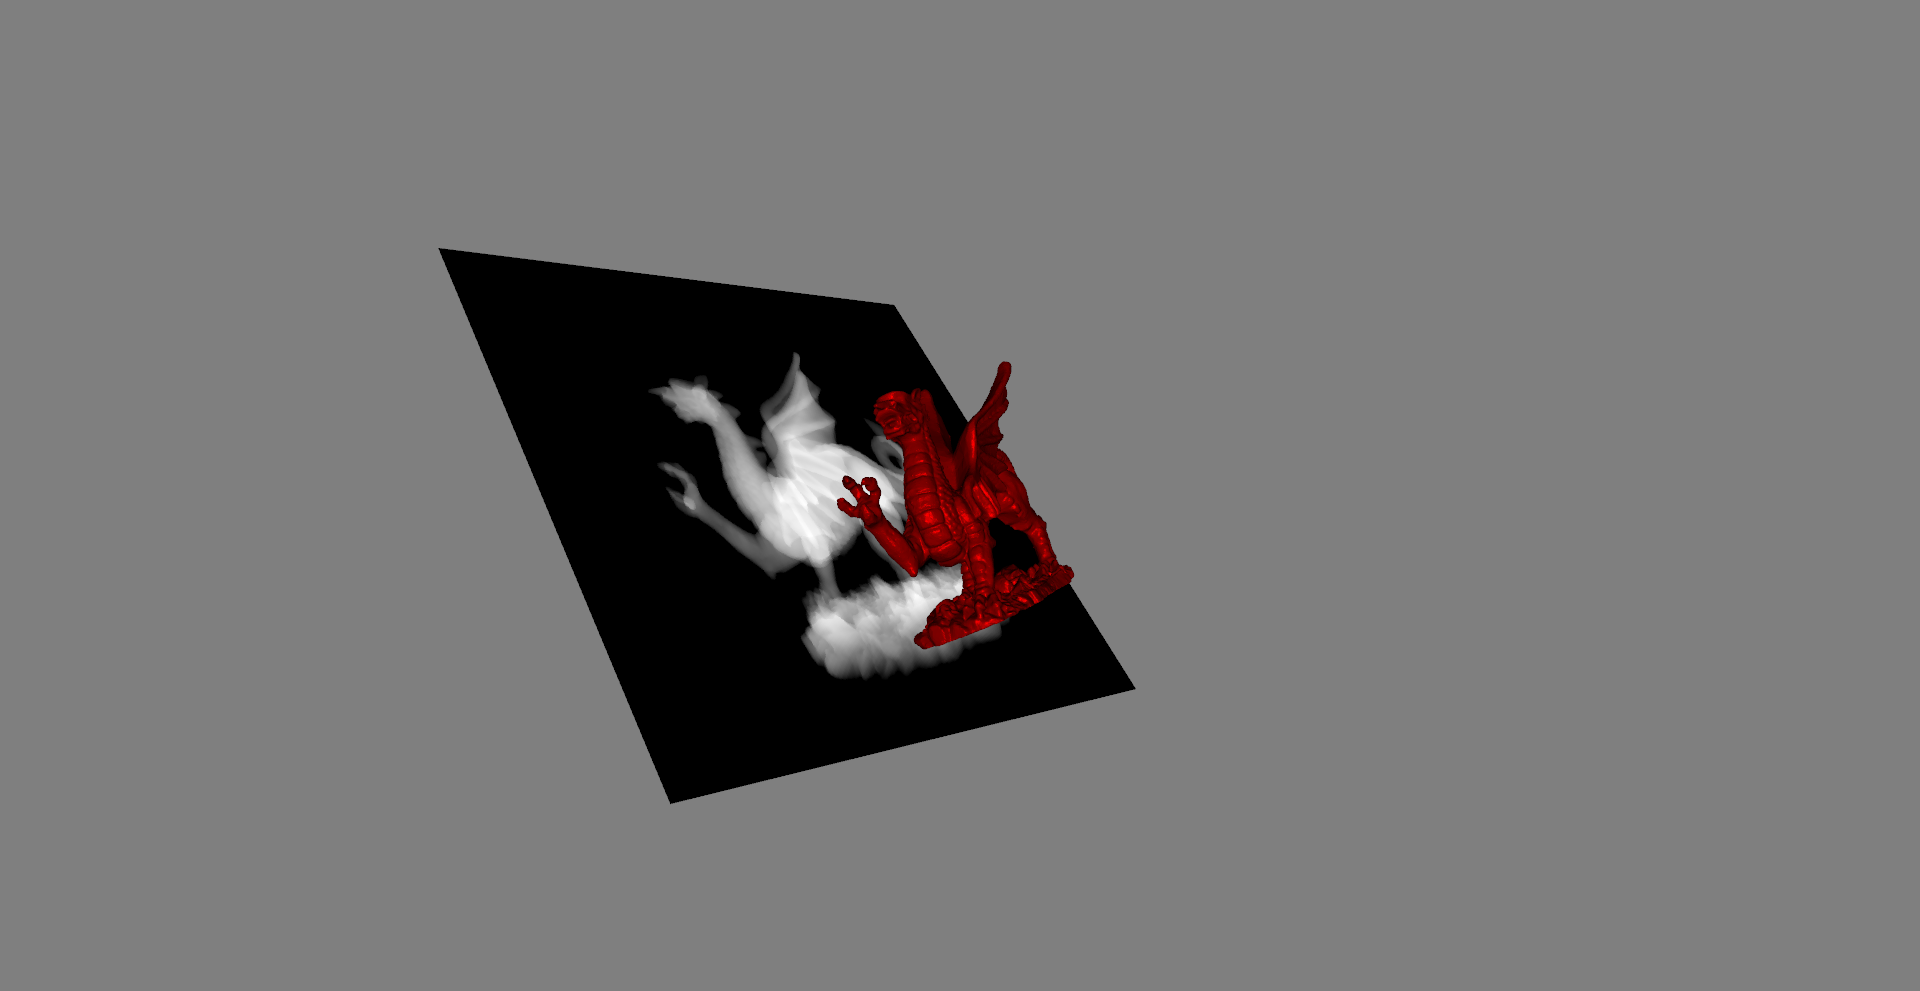
\includegraphics[width=0.25\textwidth]{mouse_right_click.png}	&	Rotate the dragon\\
		\hline
	\end{longtable}
\end{center}

\newpage
Keyboard control:
\begin{center}
    \begin{longtable}{|m{0.1\textwidth}|m{0.25\textwidth}|m{0.25\textwidth}|m{0.25\textwidth}|}
		\hline
		\textbf{Command}	&	\textbf{Before}	&	\textbf{After}	&	\multicolumn{1}{c|}{\textbf{Description}}	\\
		\hline
		\hline
		Key: \texttt{q}/\textsc{\texttt{Esc}}	&		&		&	Quit\\
		\hline
		Key: \texttt{s}	&	&	&	Stereo (on/off)\\
		\hline
		Key: \texttt{+}	&	&	&	Increase the intra ocular distance (when stereo is on)\\
		\hline
		Key: \texttt{-}	&	&	&	Decrease the intra ocular distance (when stereo is on)\\
		\hline
		Key: \texttt{i}	&	&	&	Zoom in\\
		\hline
		Key: \texttt{o}	&	&	&	Zoom out\\
		\hline
		Key: \texttt{b}	&	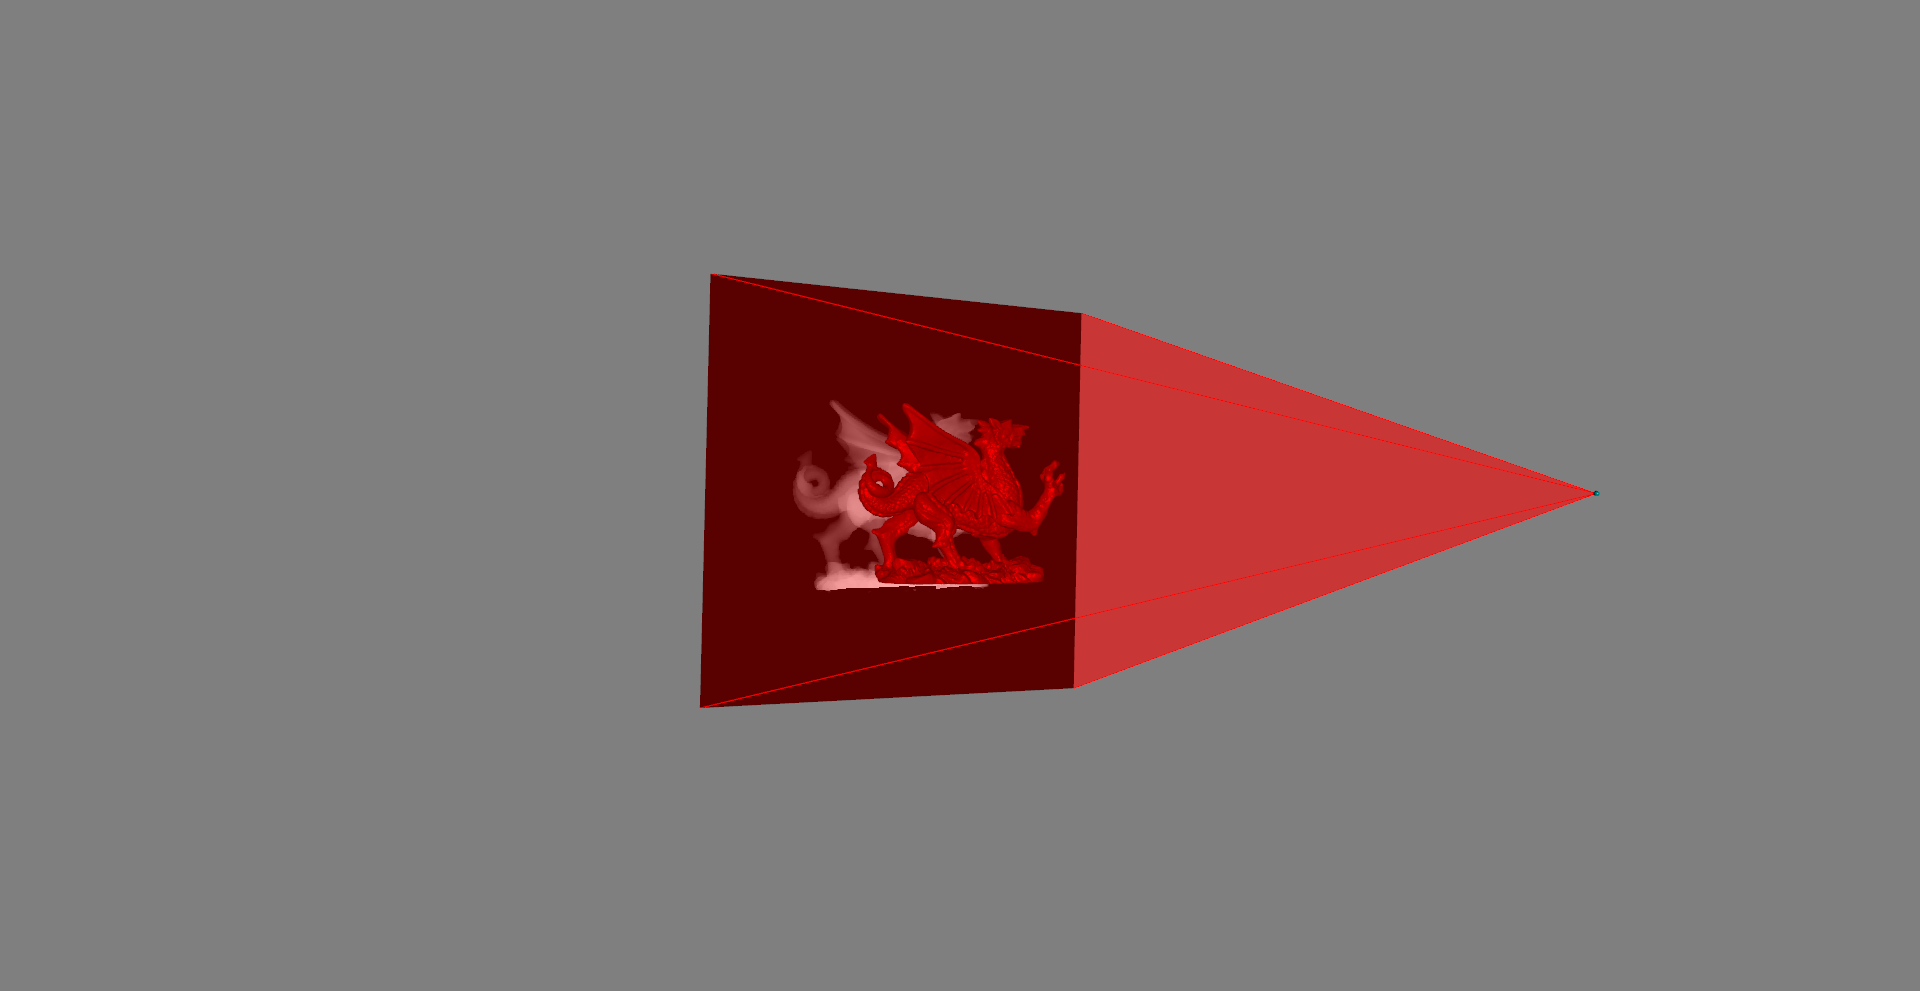
\includegraphics[width=0.25\textwidth]{beam_on.png}	&	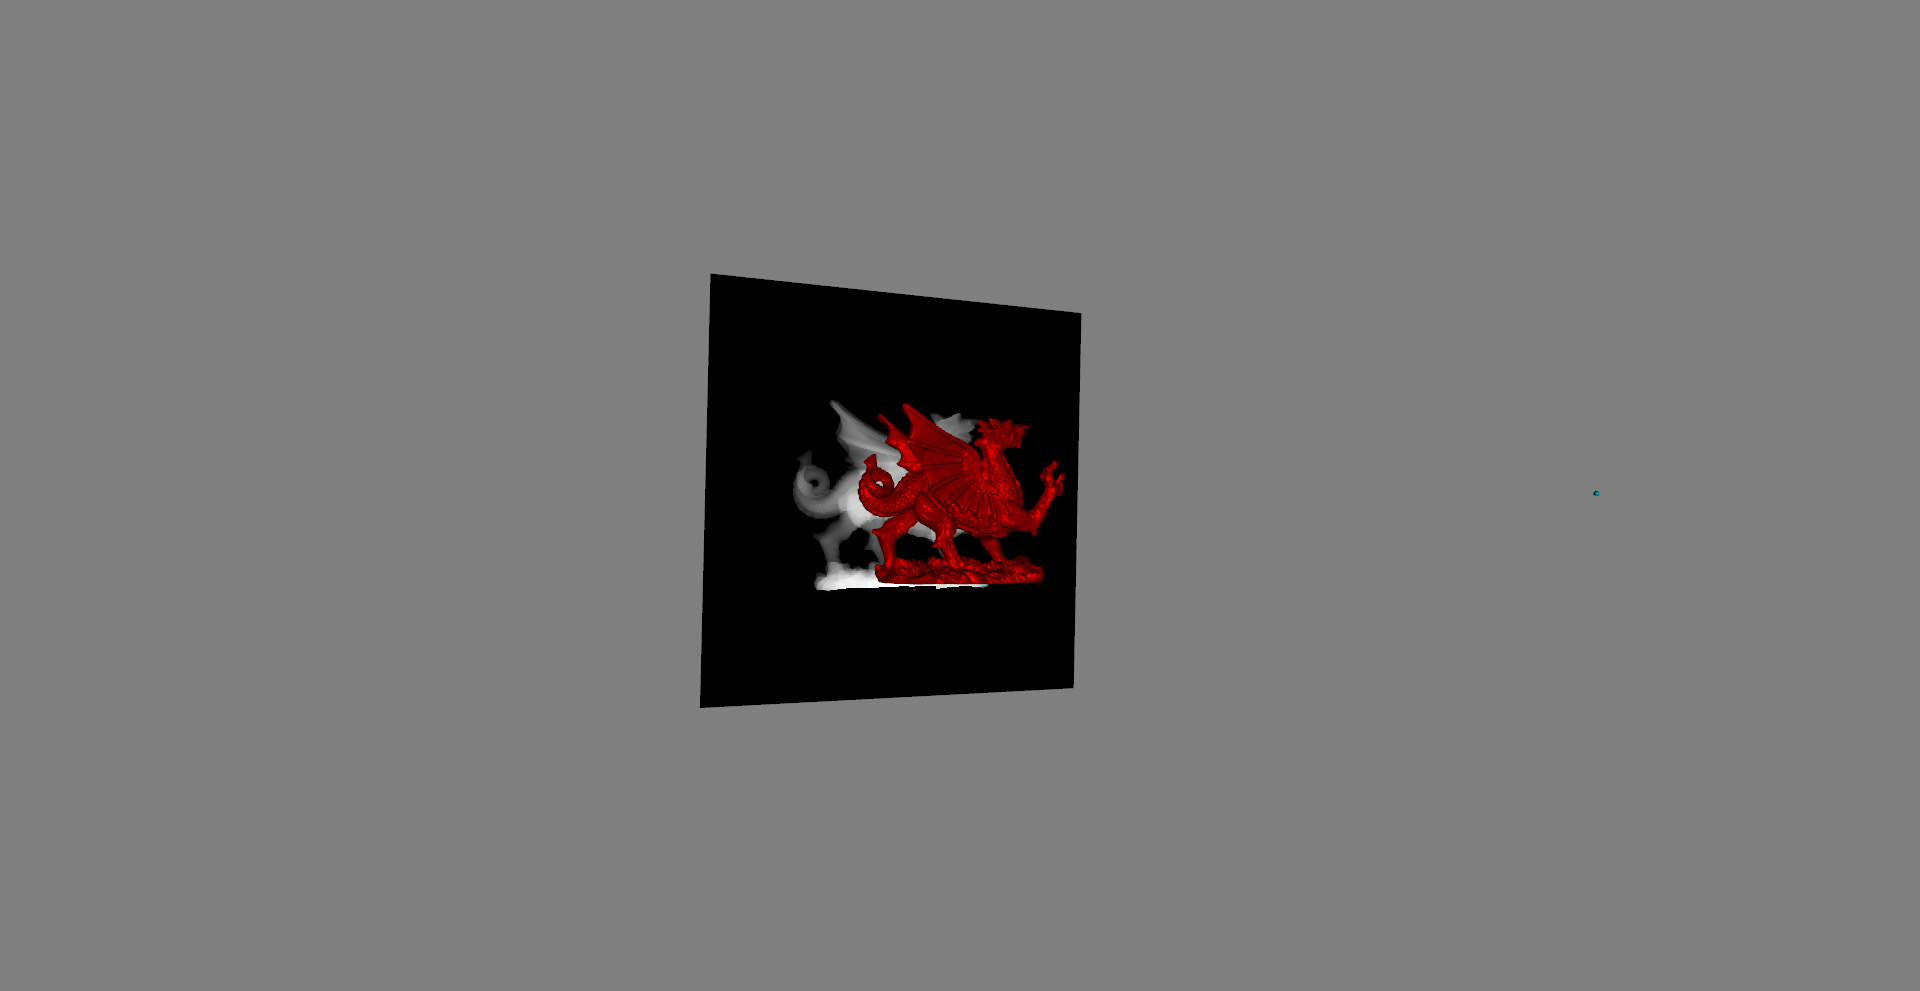
\includegraphics[width=0.25\textwidth]{beam_off.png}	&	Display the X-ray beam (on/off)\\
		\hline
		Key: \texttt{n}	&	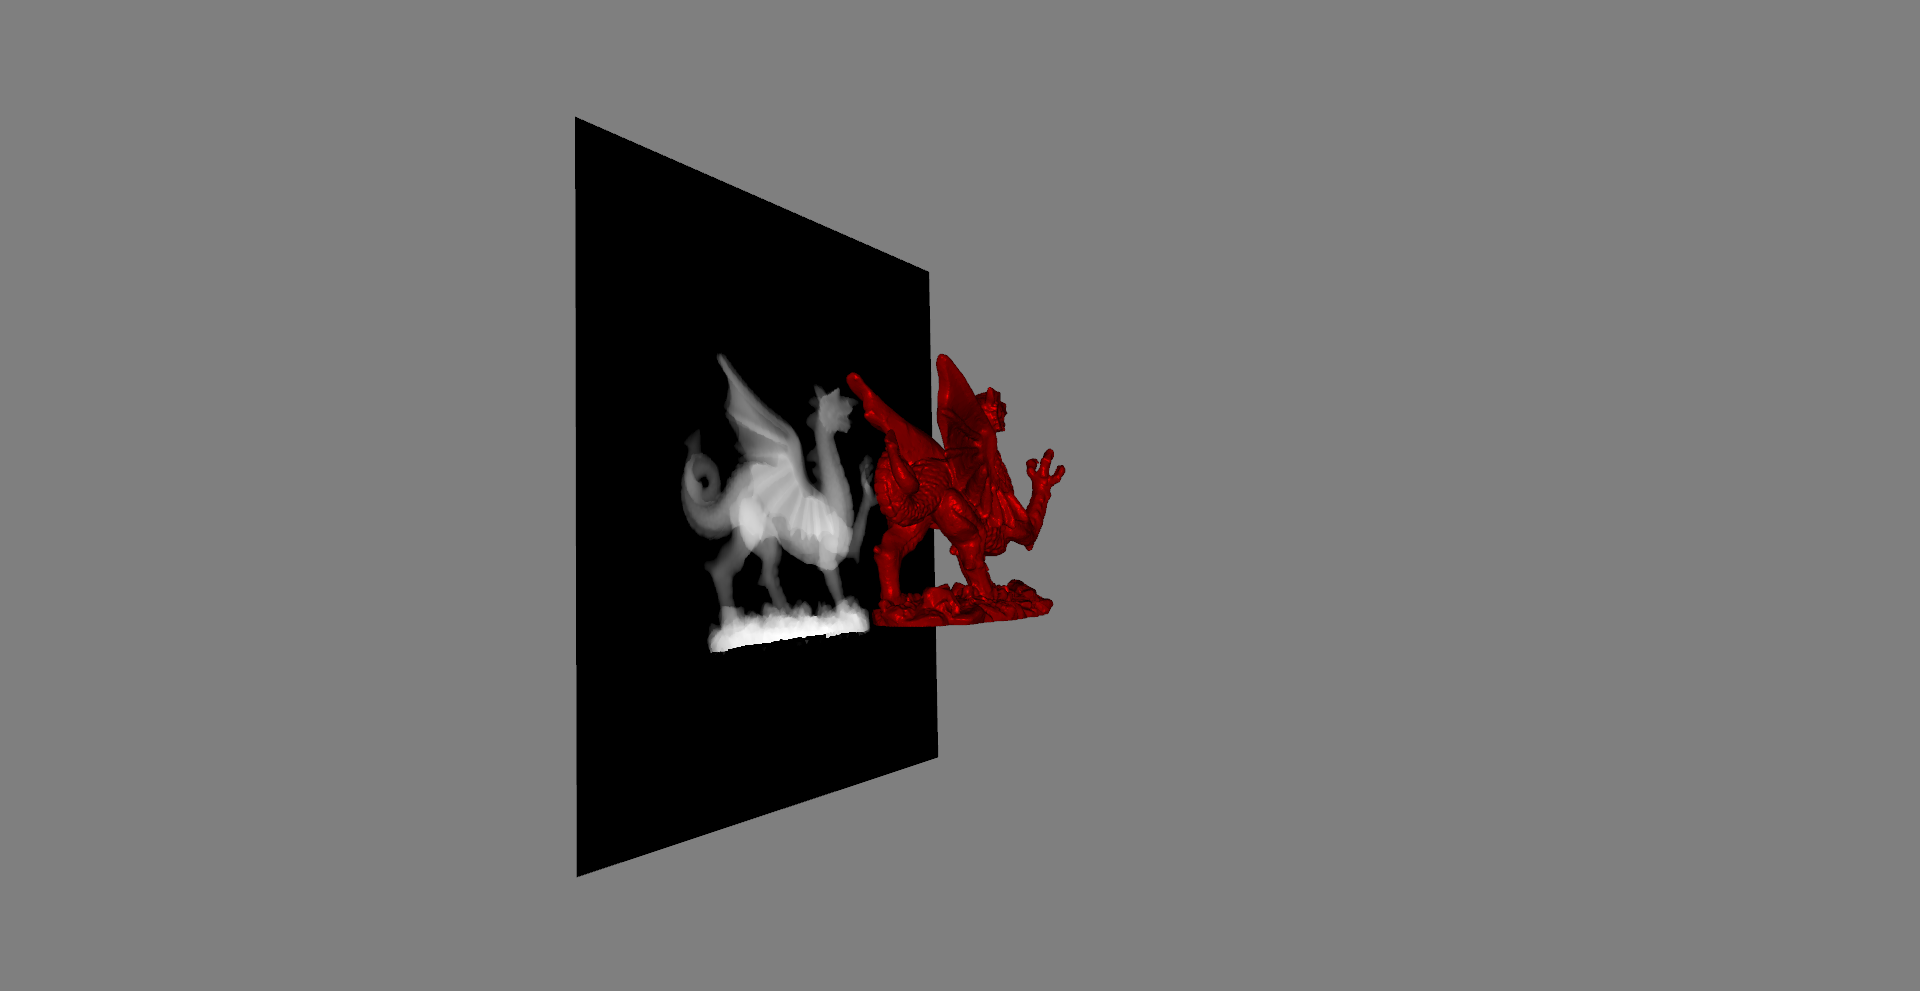
\includegraphics[width=0.25\textwidth]{negative_on.png}	&	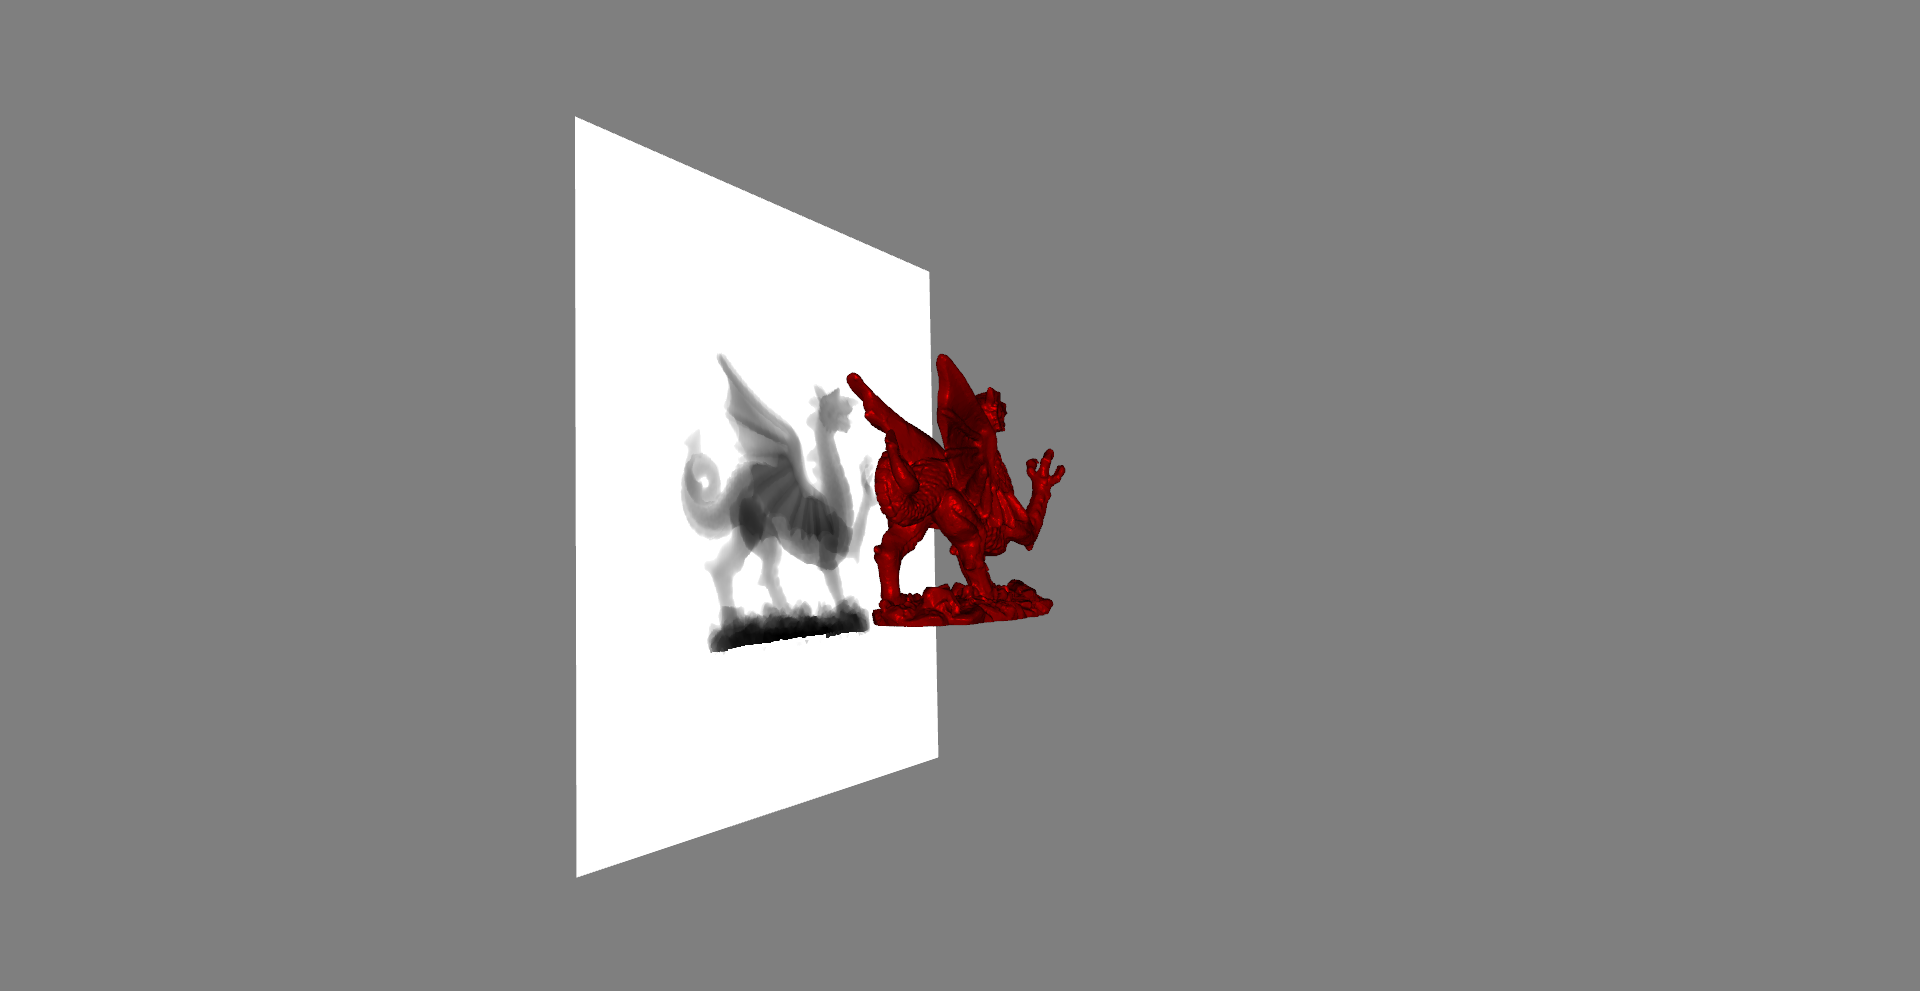
\includegraphics[width=0.25\textwidth]{negative_off.png}	&	Display the X-ray in negative (on/off)\\
		\hline
		Key: \texttt{w}	&	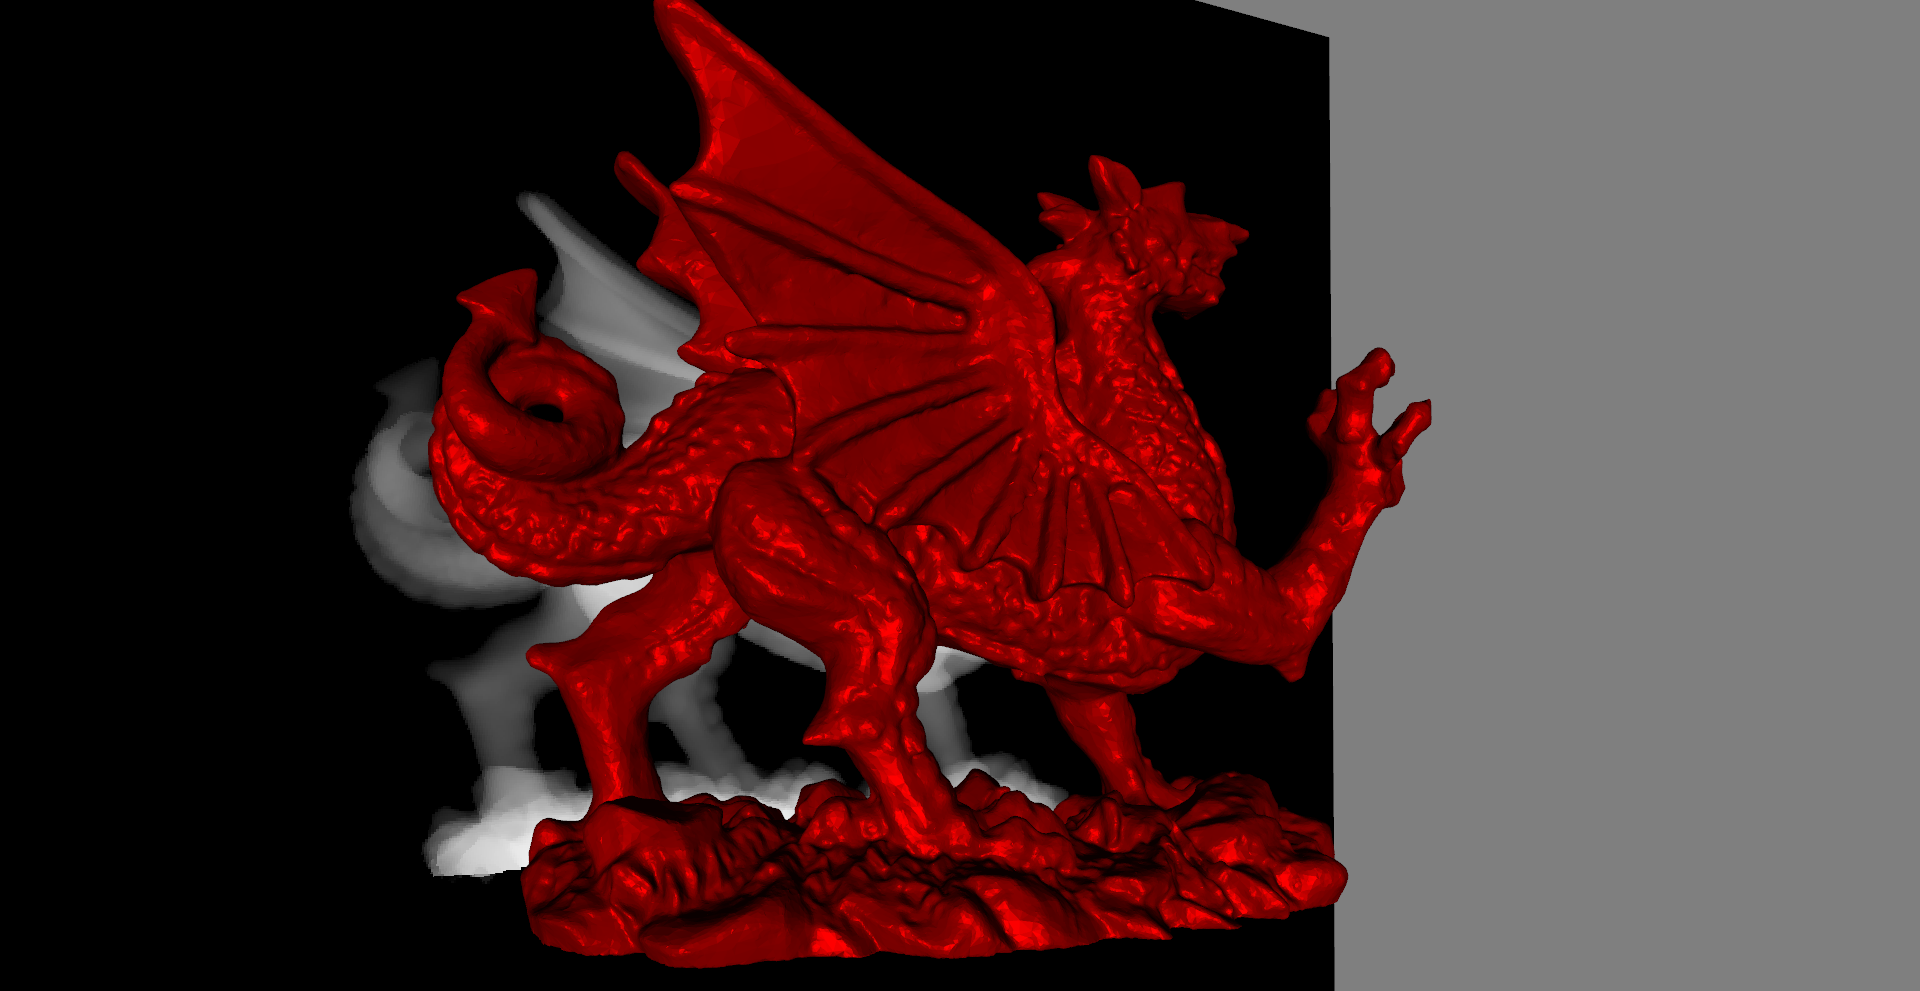
\includegraphics[width=0.25\textwidth]{solid_model.png}	&	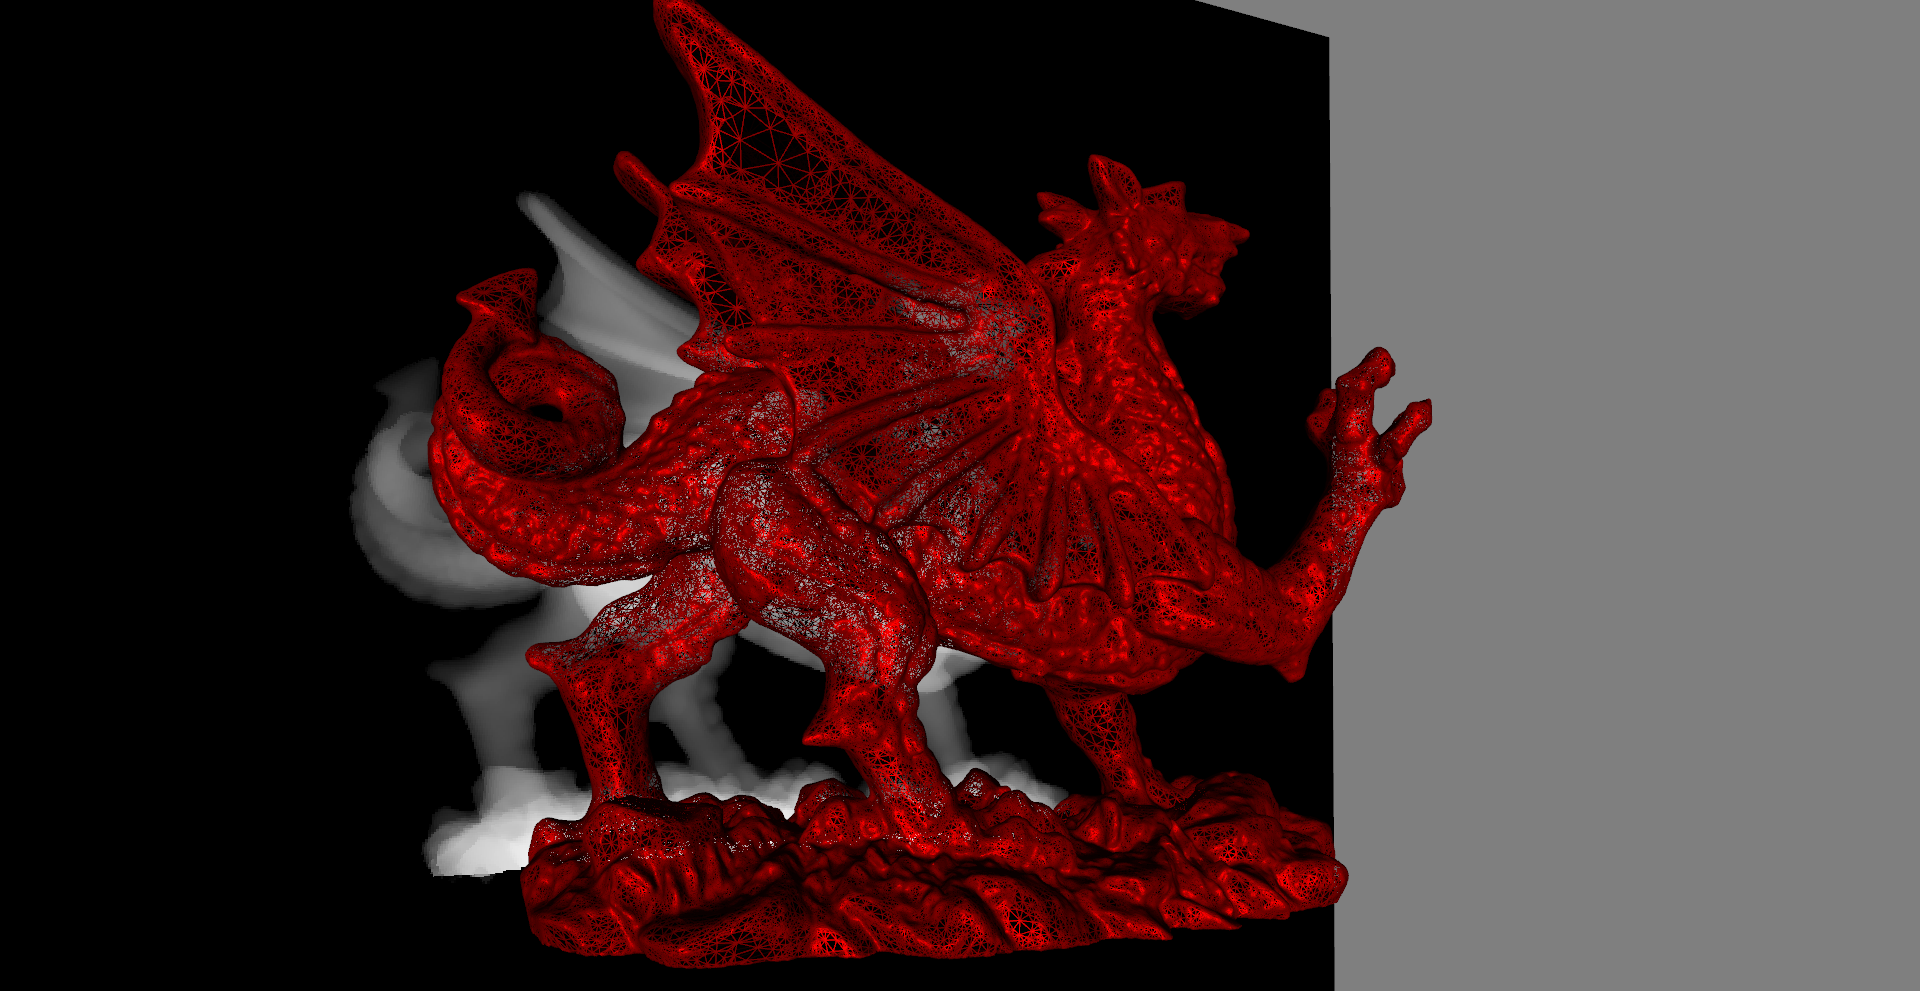
\includegraphics[width=0.25\textwidth]{wireframe_model.png}	&	Display the dragon in wireframe (on/off)\\
		\hline
		Key: \texttt{1}	&	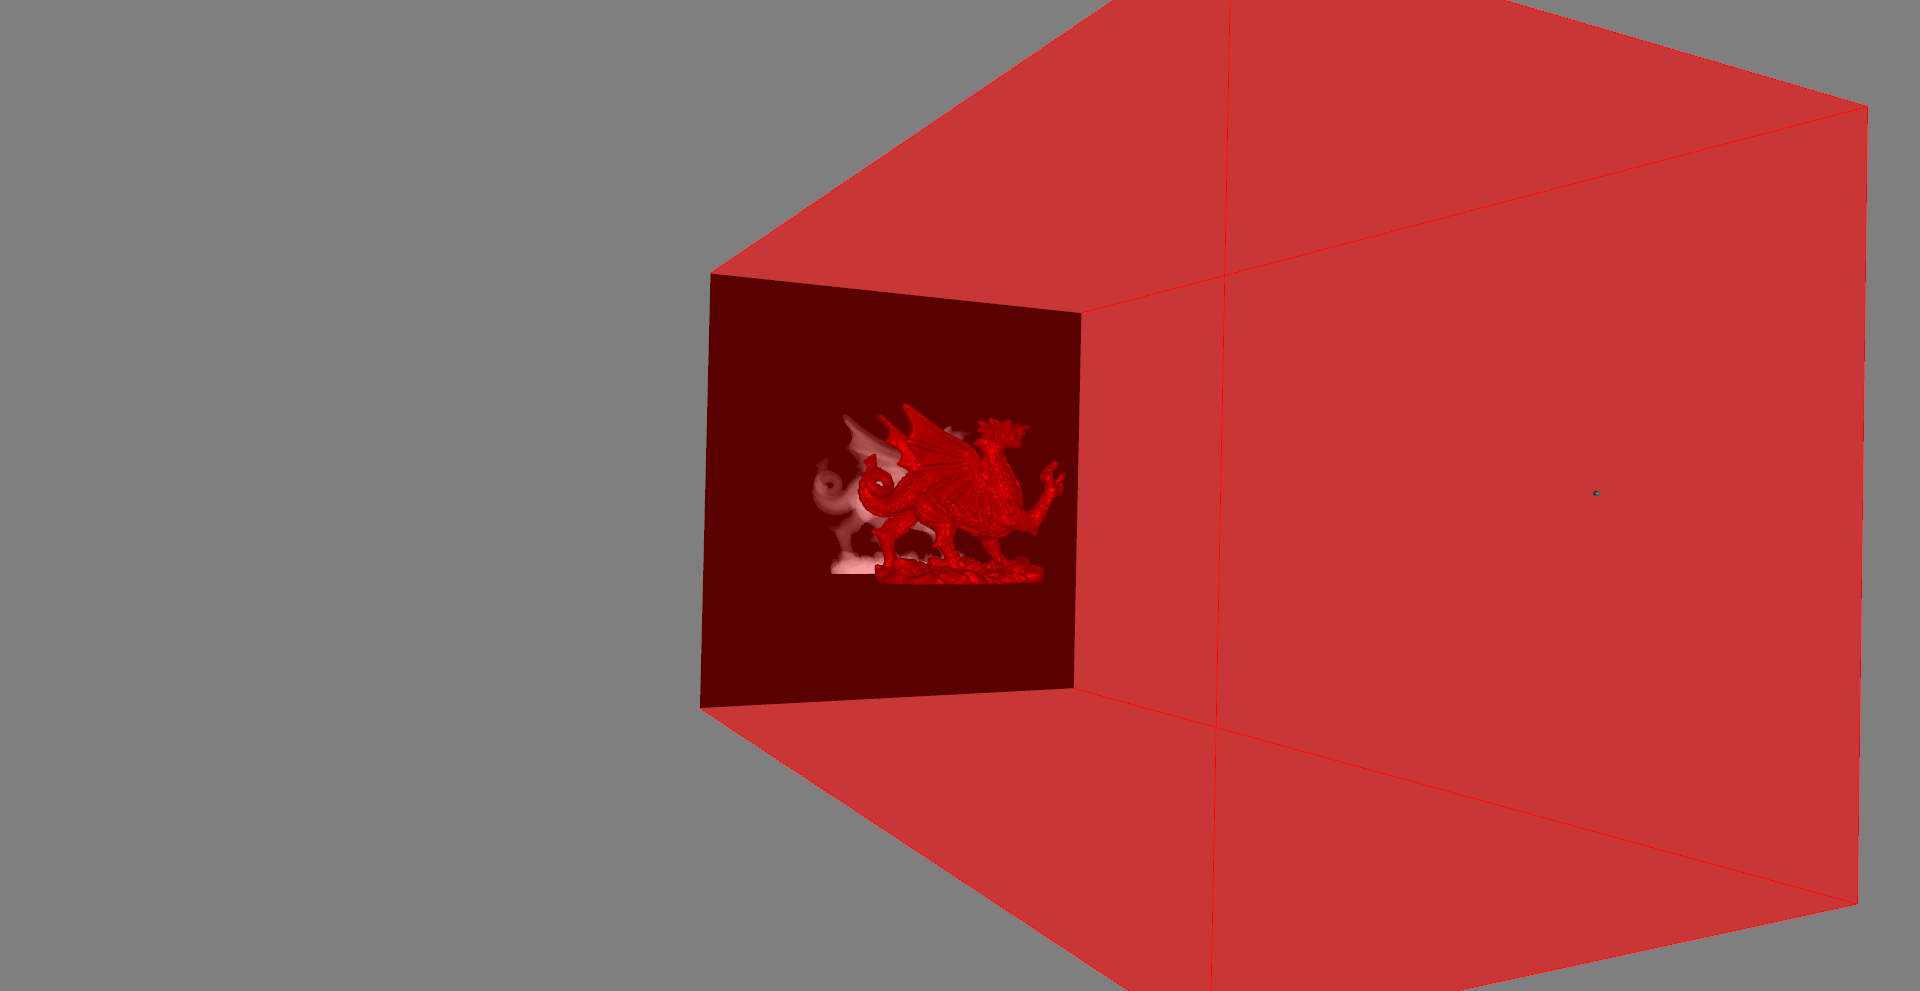
\includegraphics[width=0.25\textwidth]{parallel_beam.png}	&	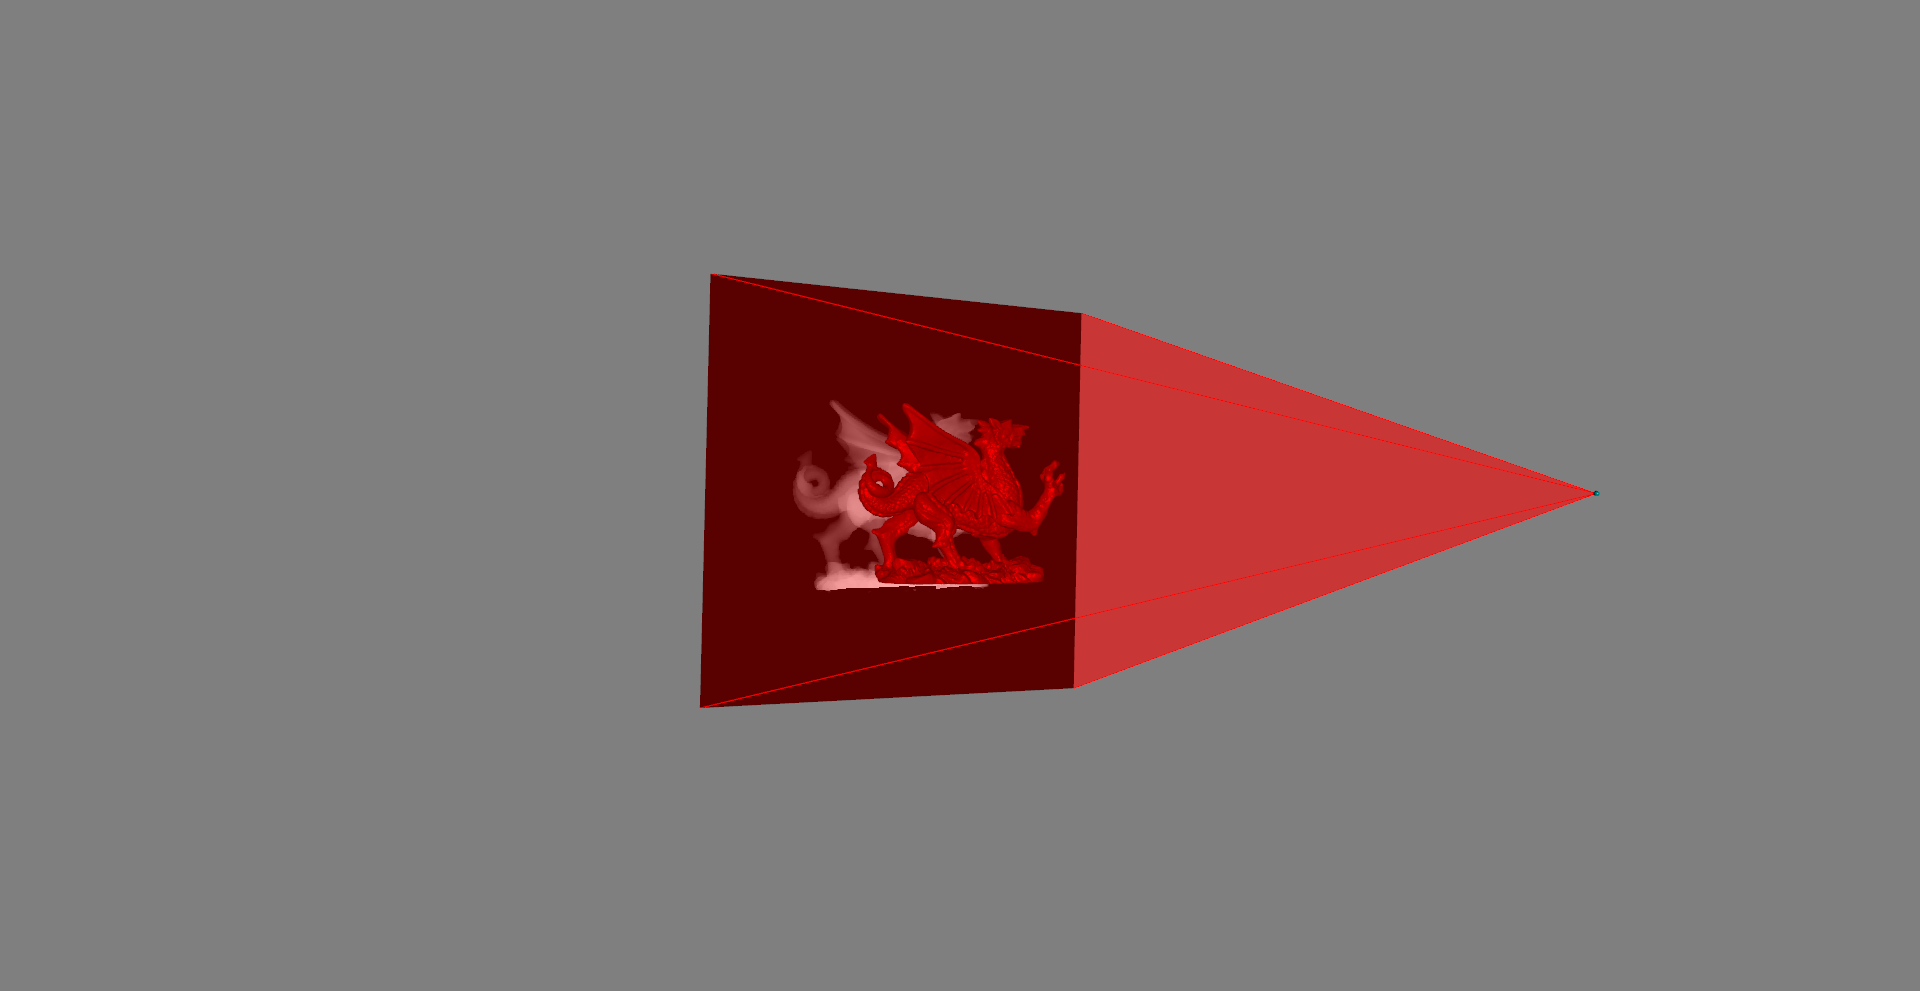
\includegraphics[width=0.25\textwidth]{point_source.png}	&	Use a parallel beam/Use a point source\\
		\hline
		\multirow{2}{*}{Key: \texttt{2}}	&	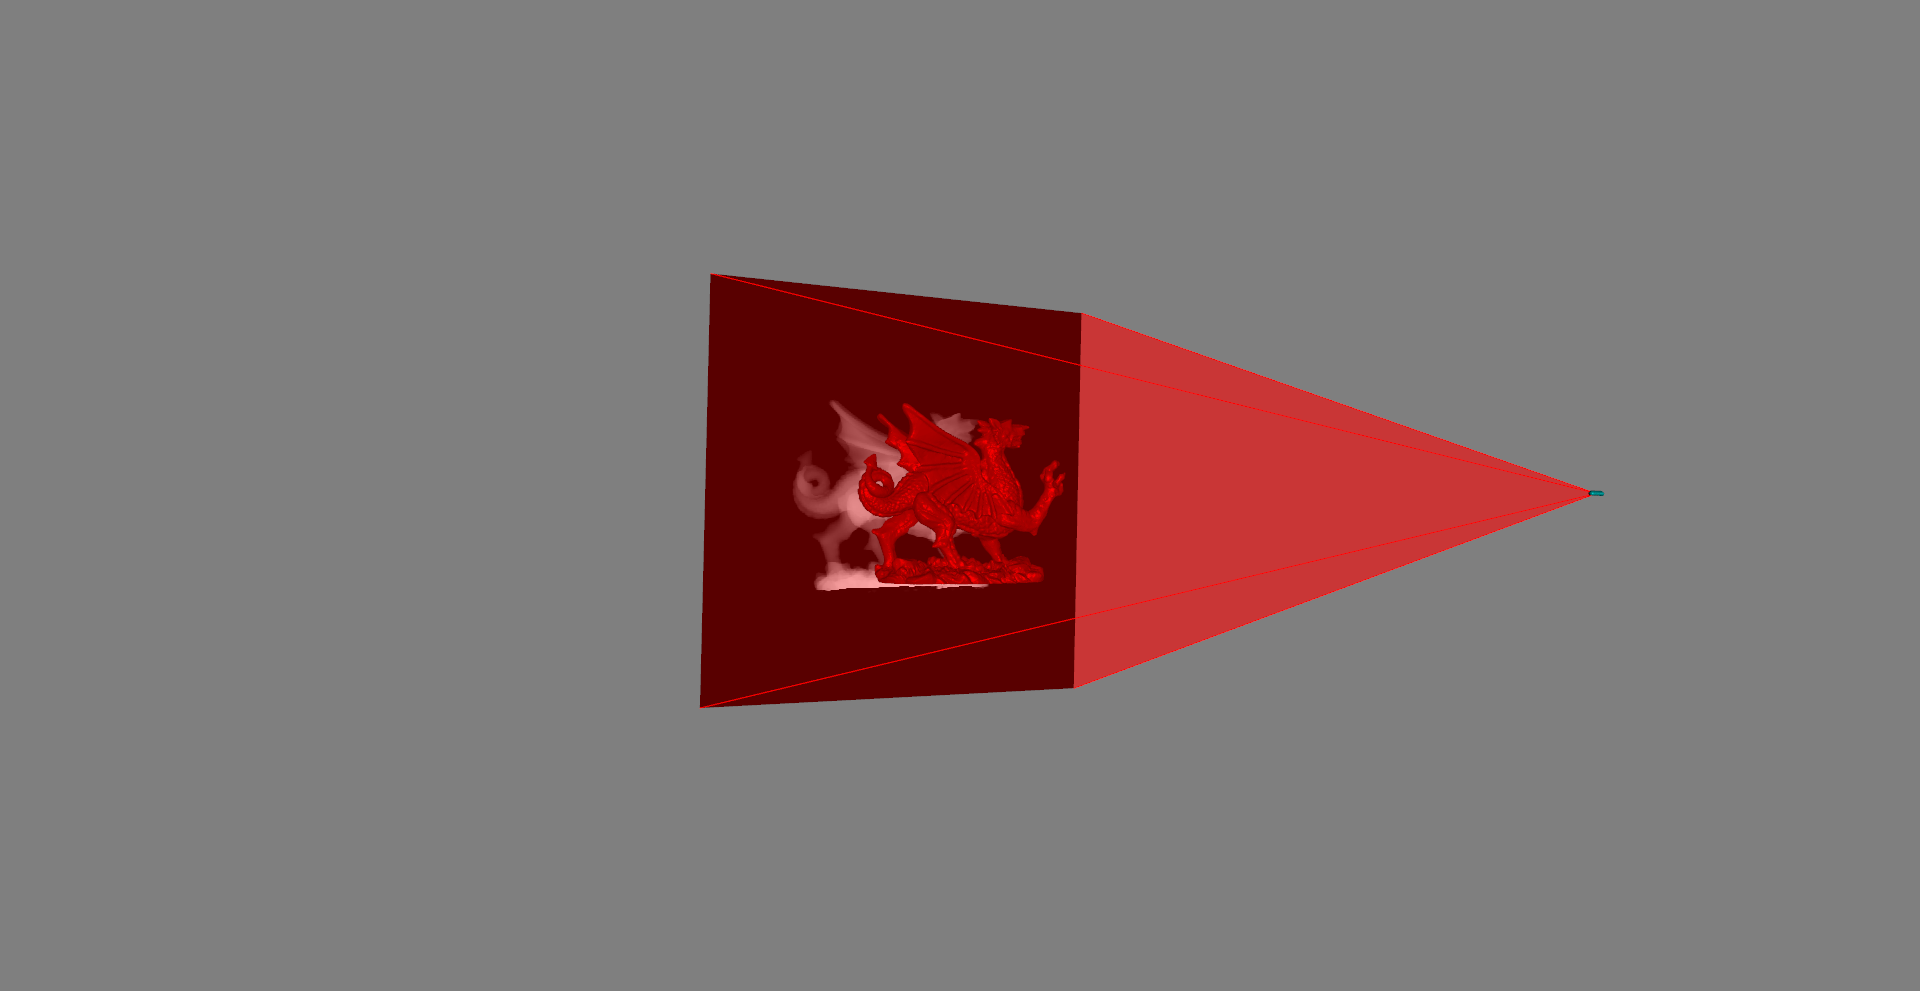
\includegraphics[width=0.25\textwidth]{line_source.png}	&	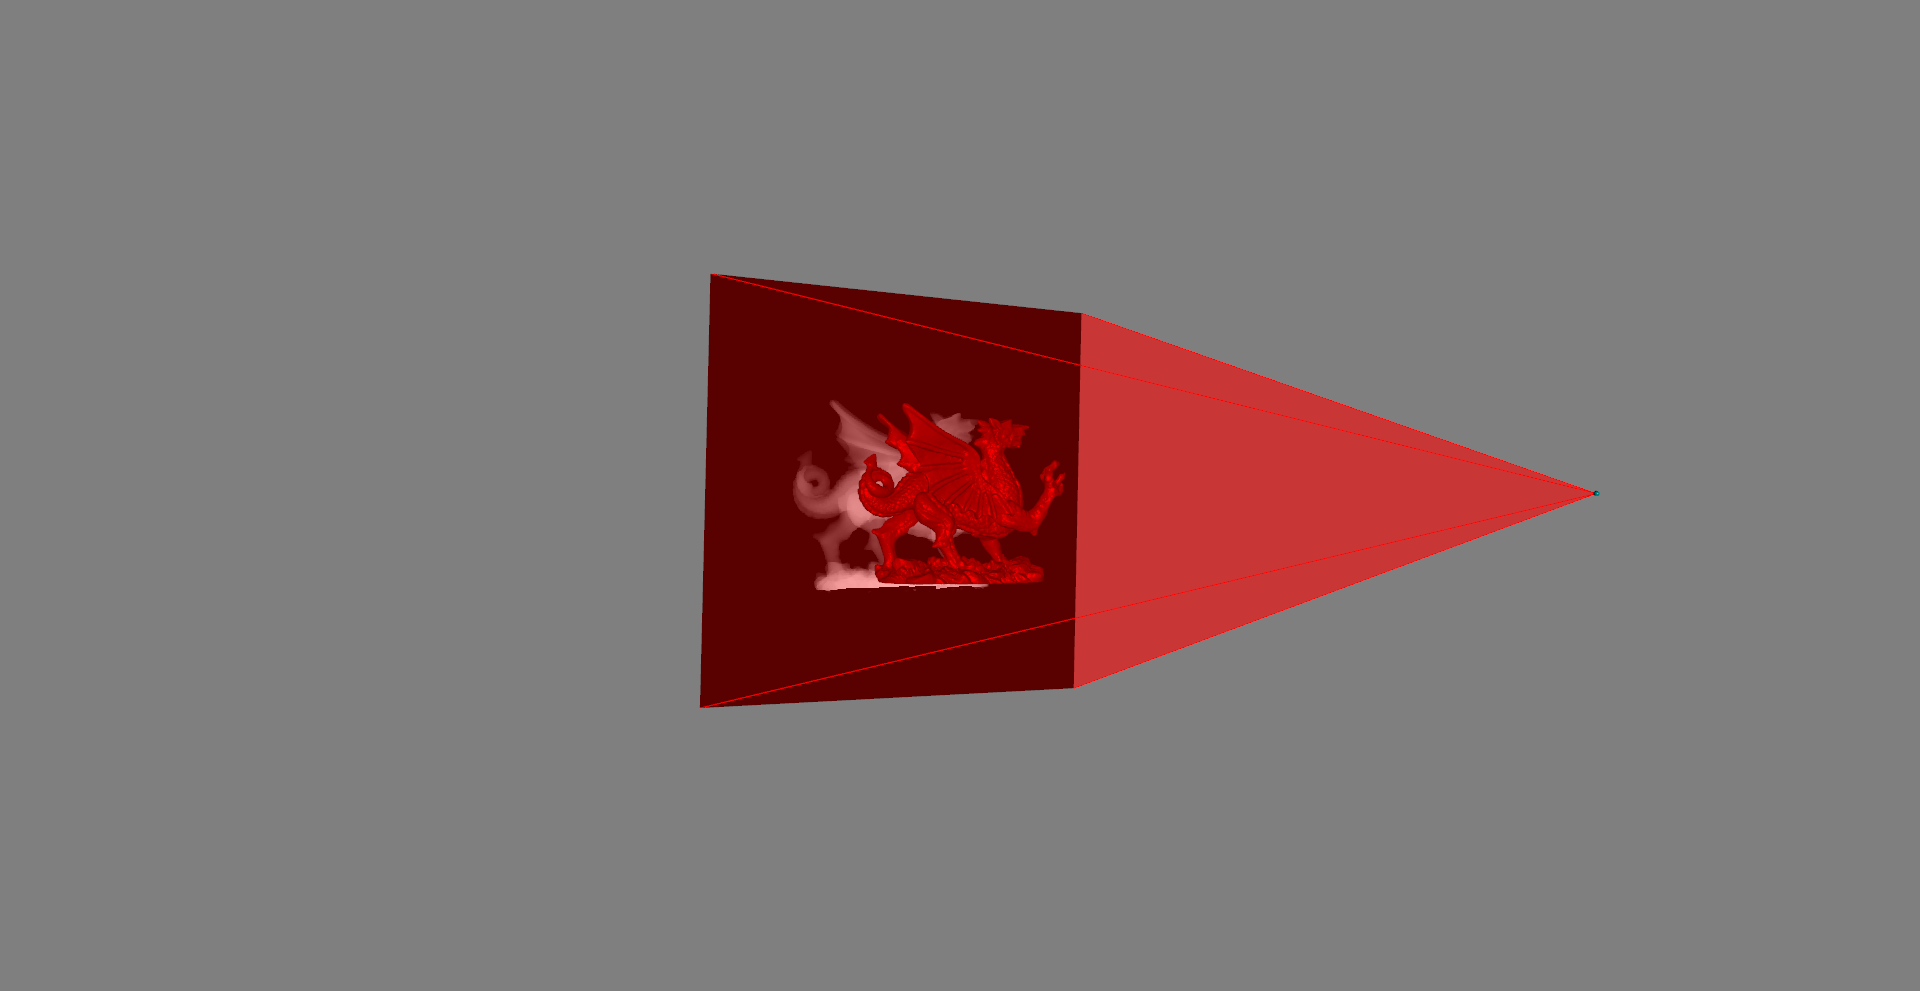
\includegraphics[width=0.25\textwidth]{point_source.png}	&	Use a line source/Use a point source\\
			&	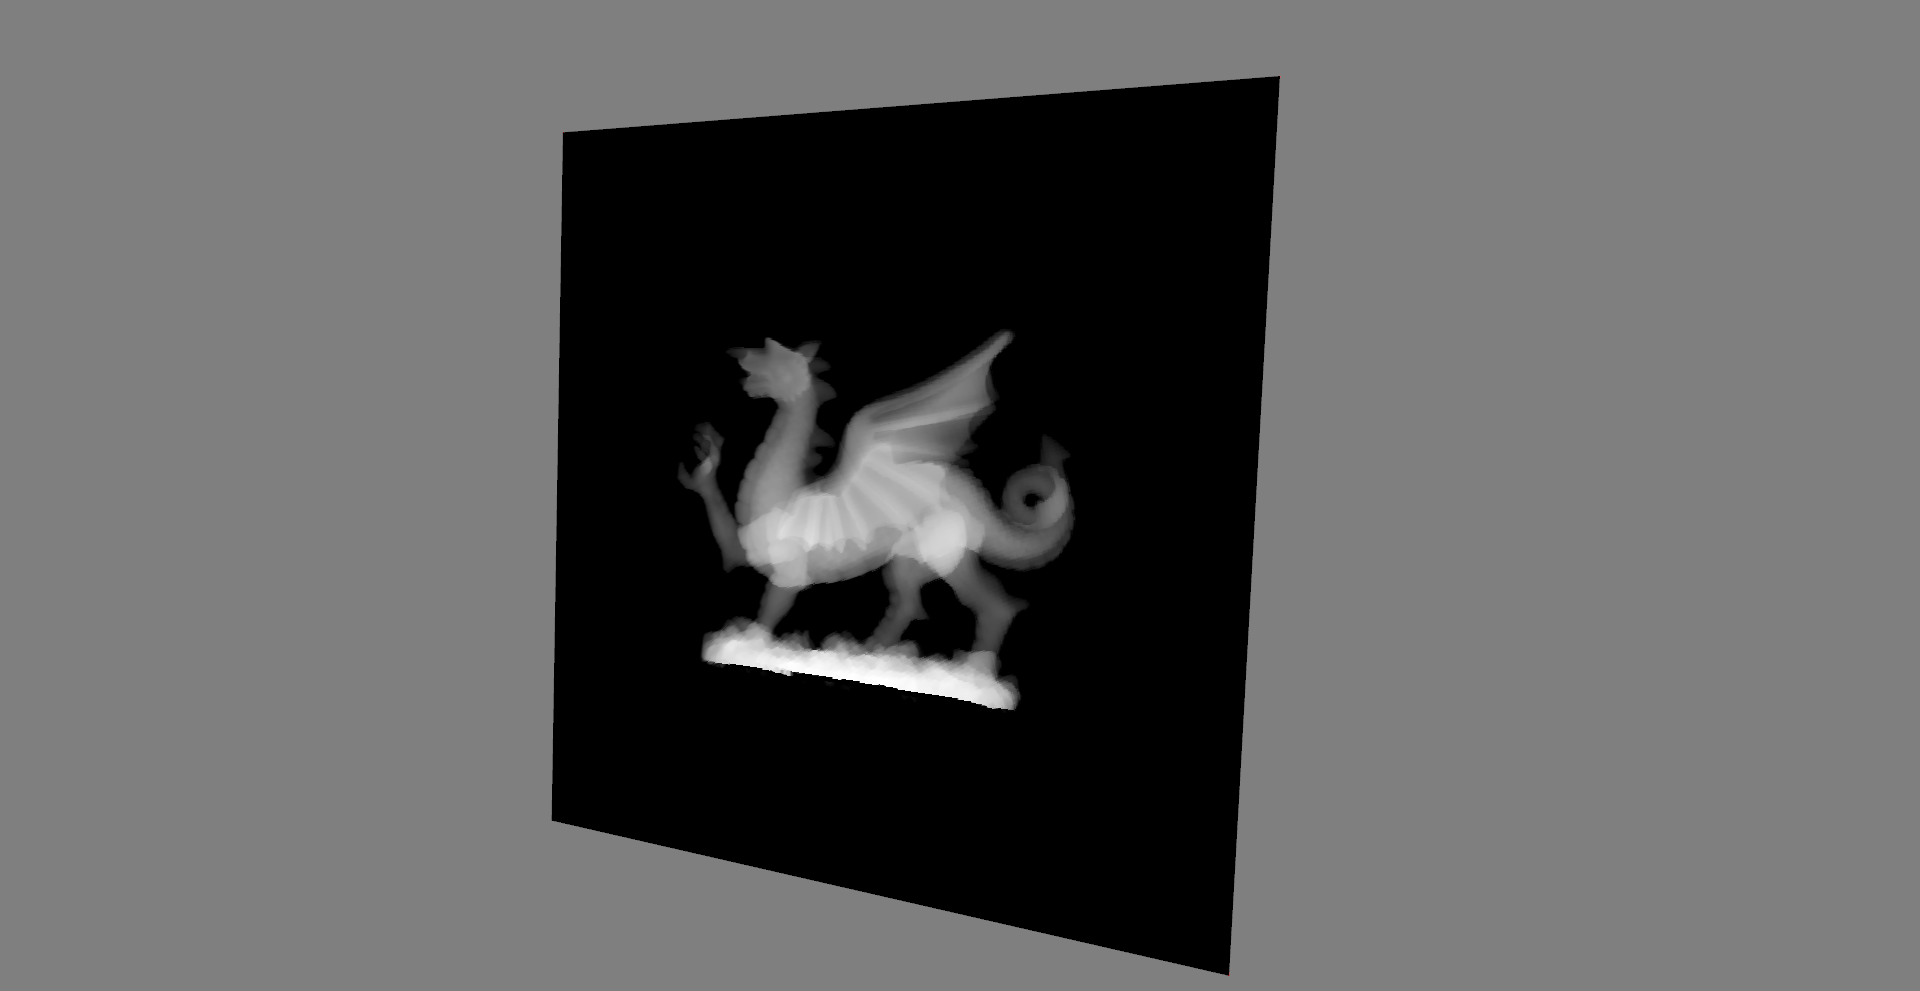
\includegraphics[width=0.25\textwidth]{line_source_xray.png}	&	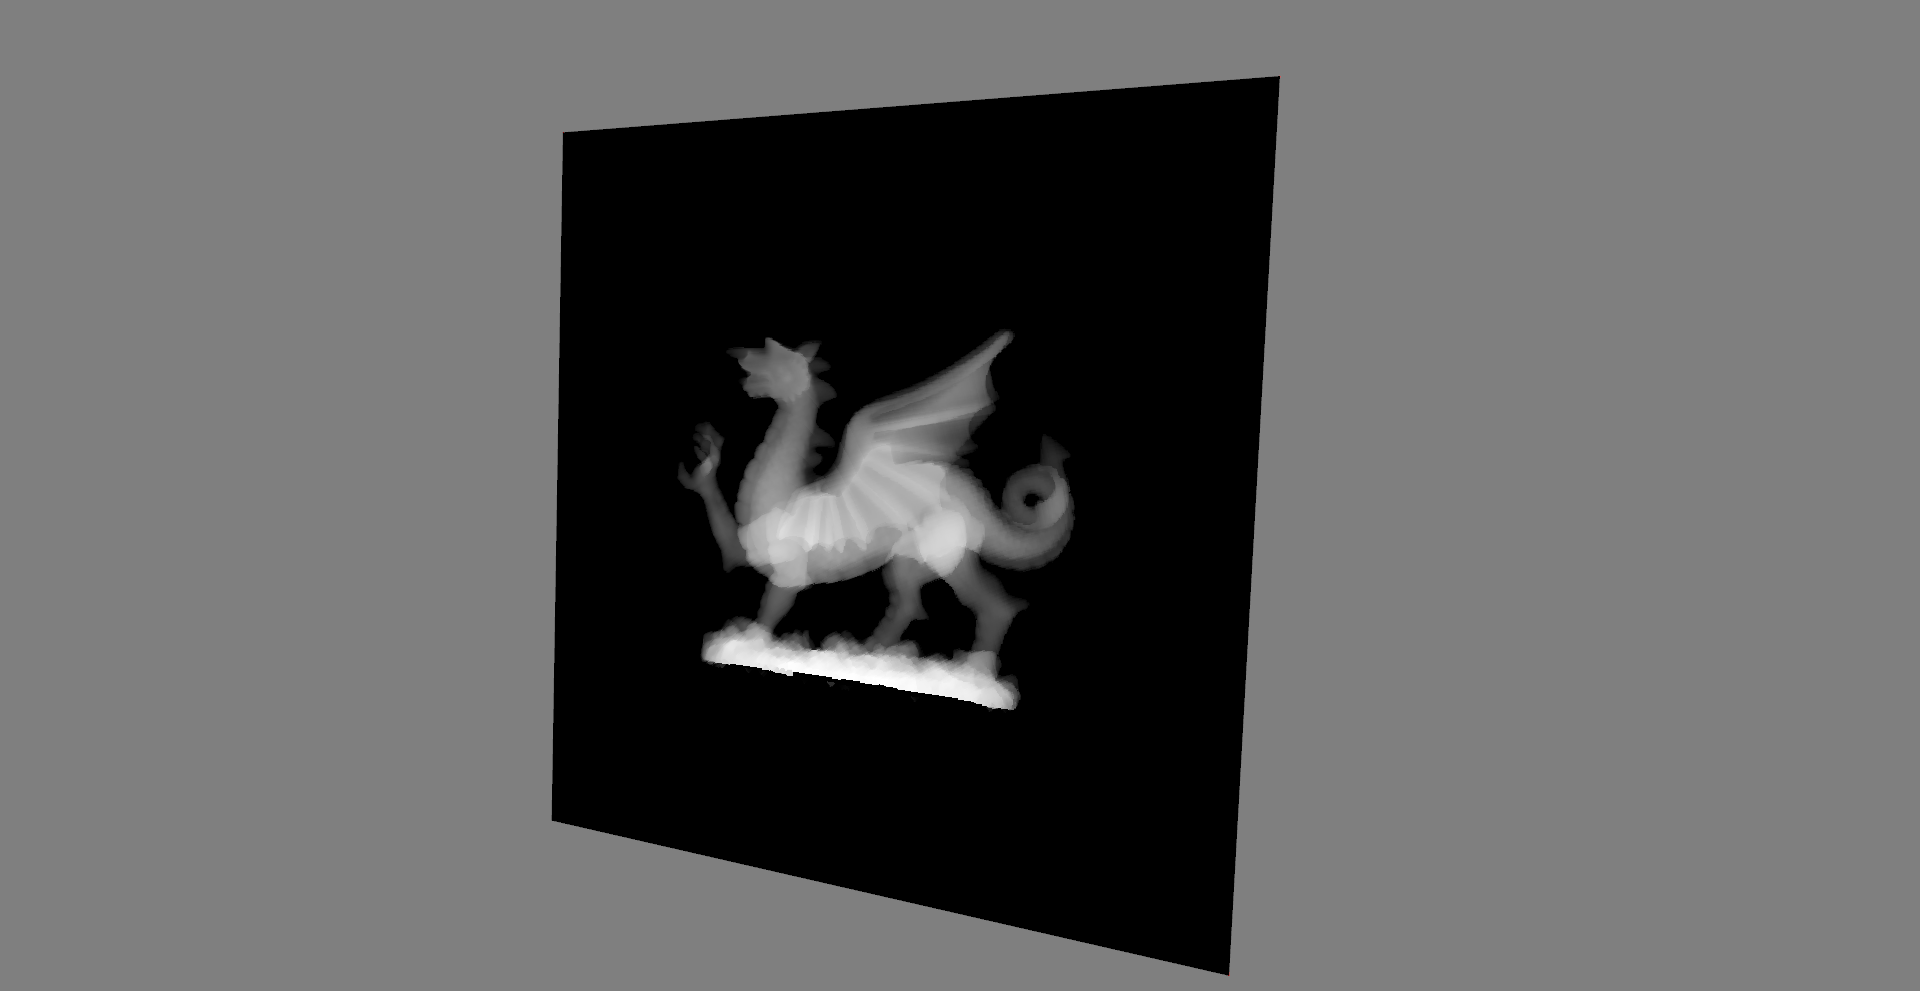
\includegraphics[width=0.25\textwidth]{point_source_xray.png}	&	(the image on the right-hand side is sharper) \\
		\hline
		\multirow{2}{*}{Key: \texttt{3}}	&	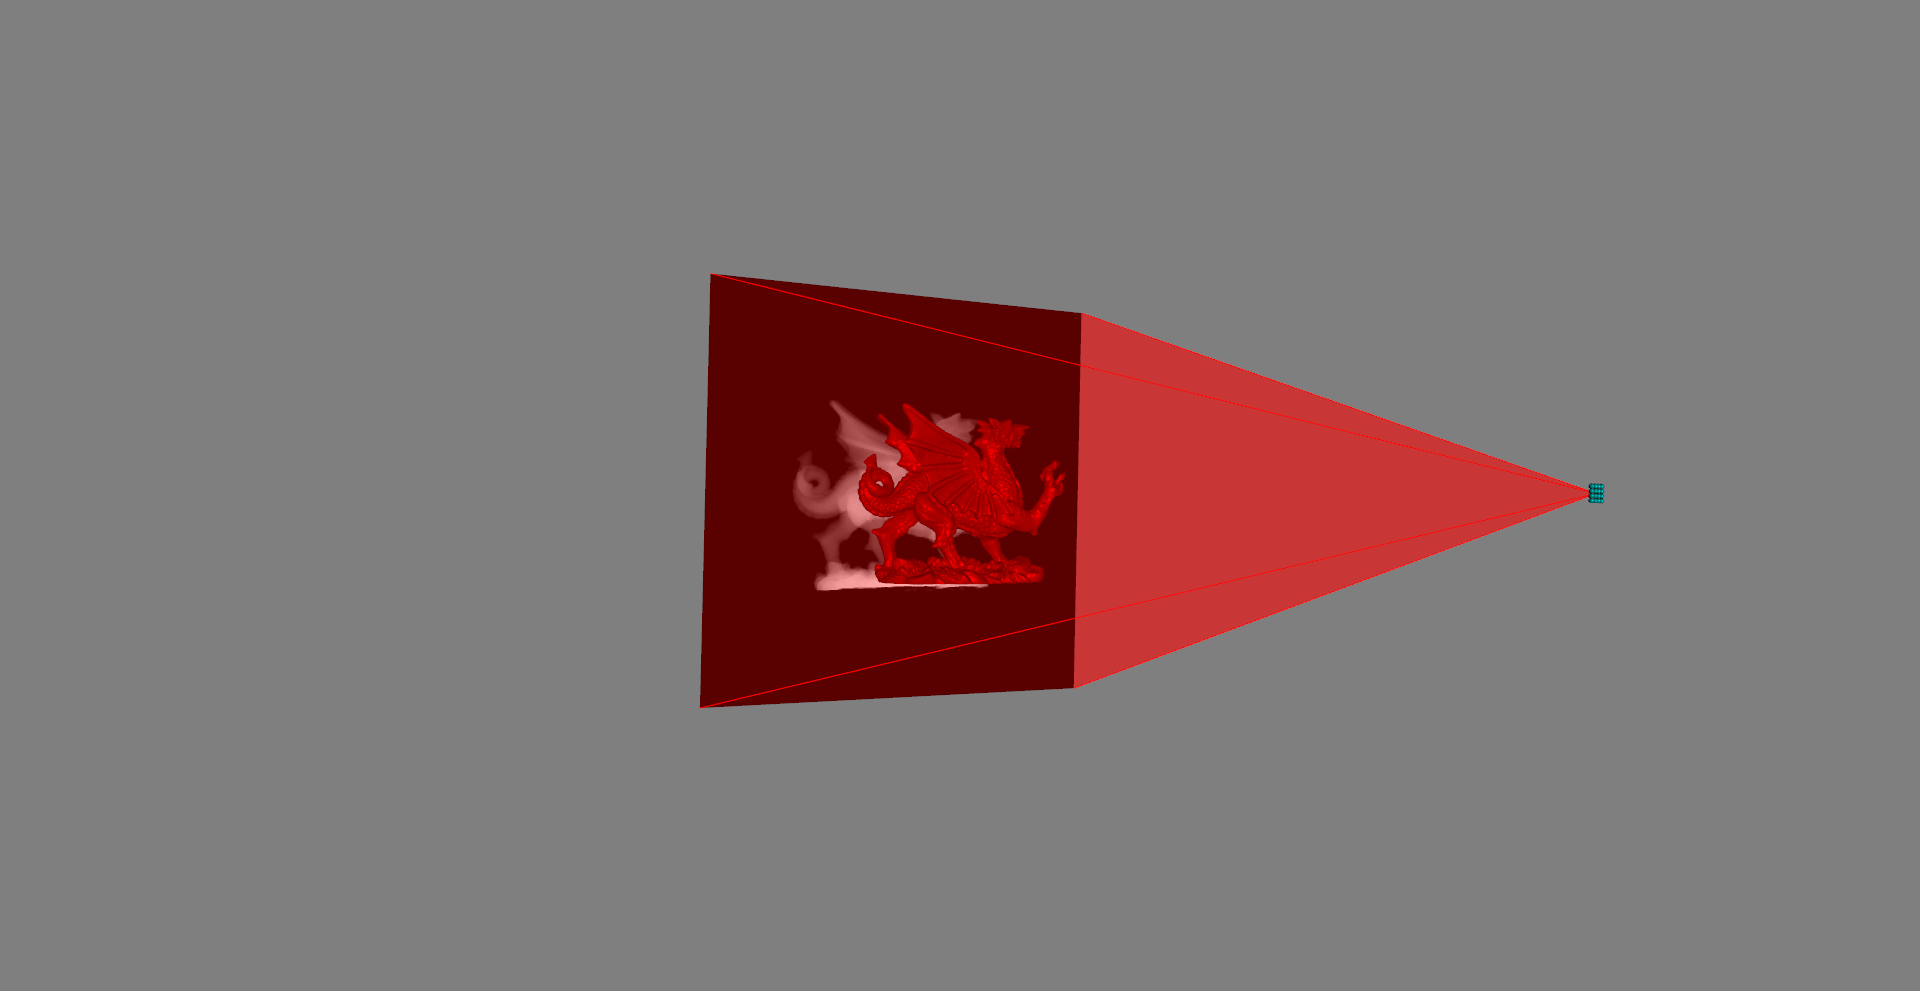
\includegraphics[width=0.25\textwidth]{square_source.png}	&	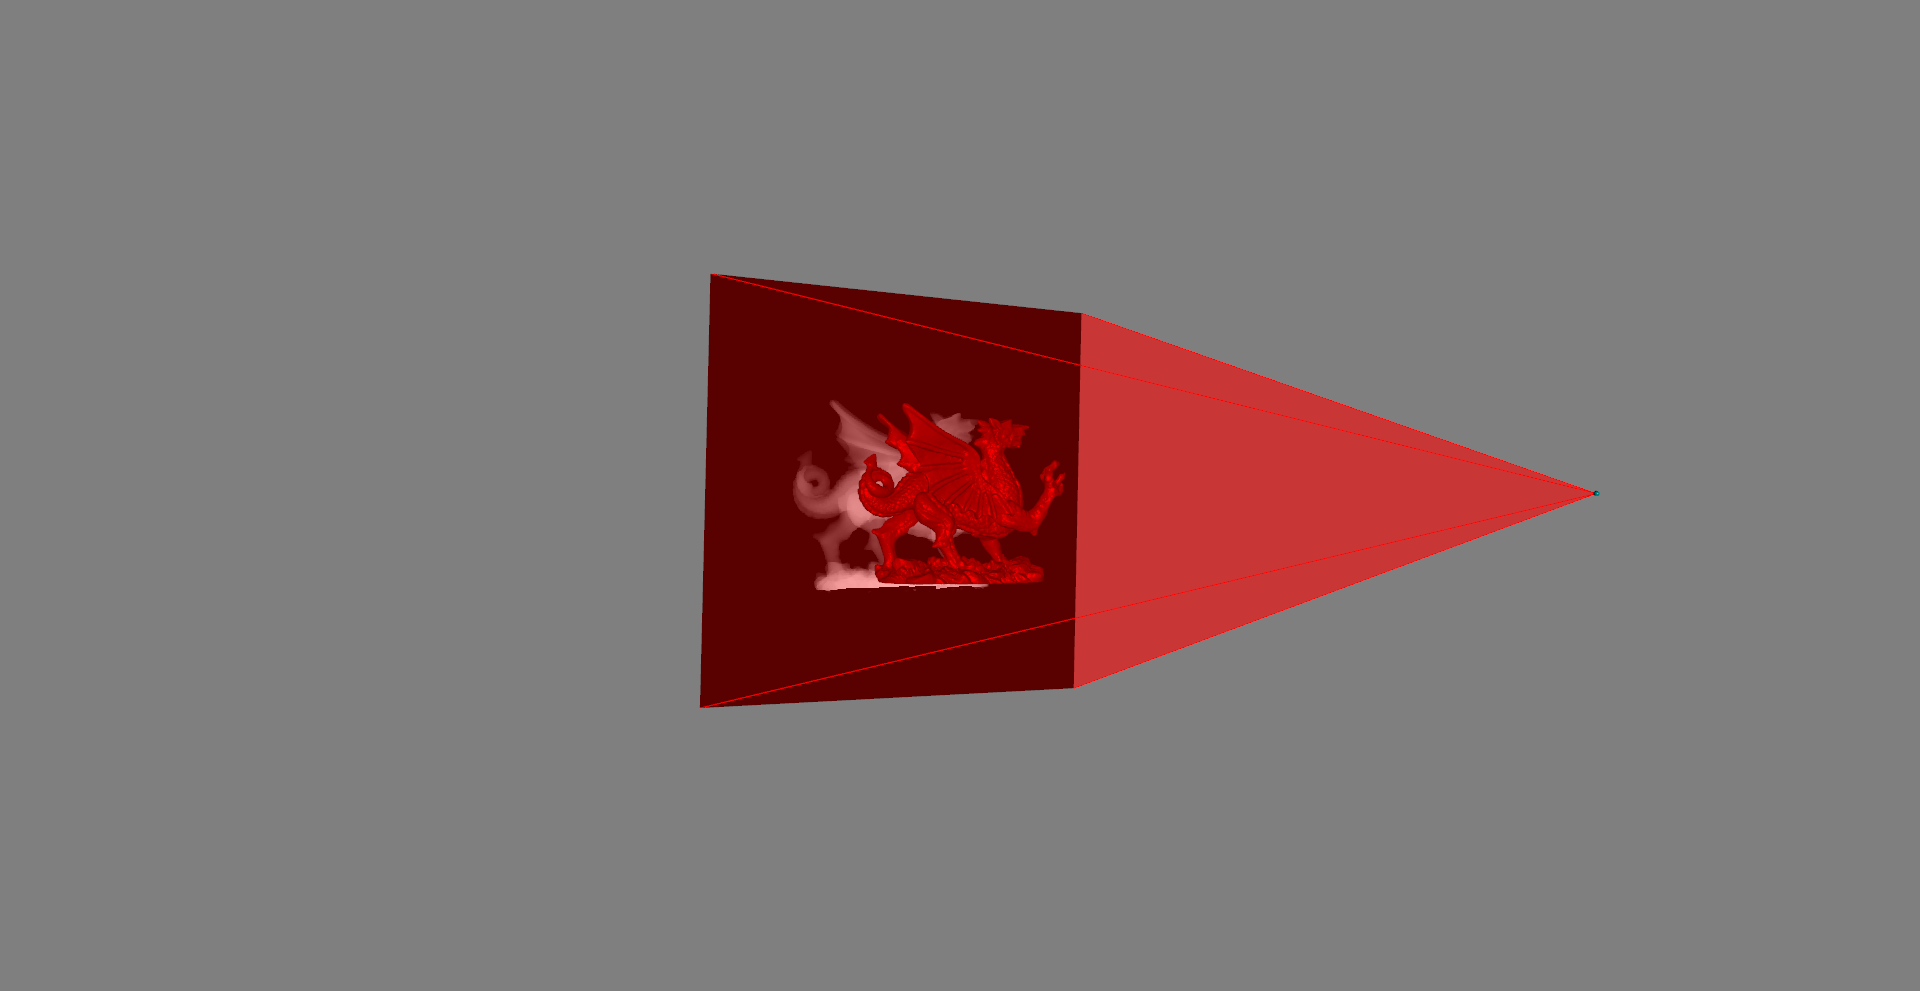
\includegraphics[width=0.25\textwidth]{point_source.png}	&	Use a square source/Use a point source\\
			&	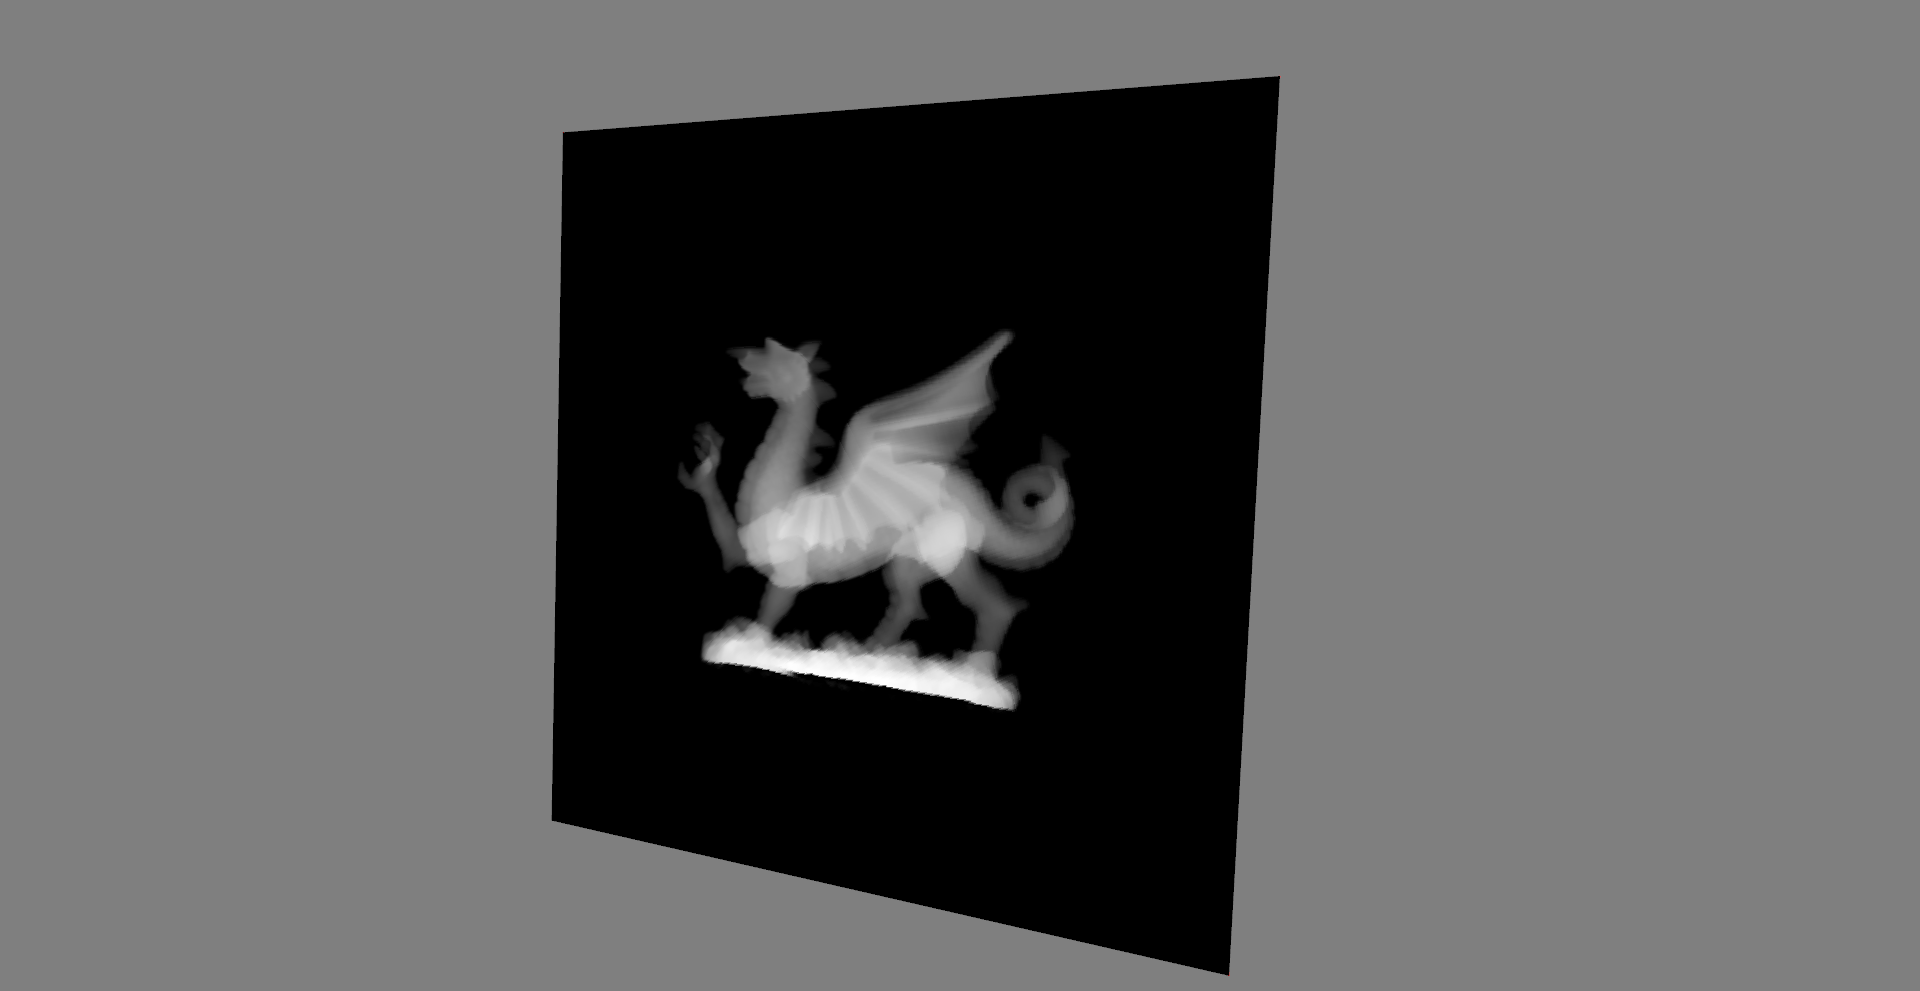
\includegraphics[width=0.25\textwidth]{square_source_xray.png}	&	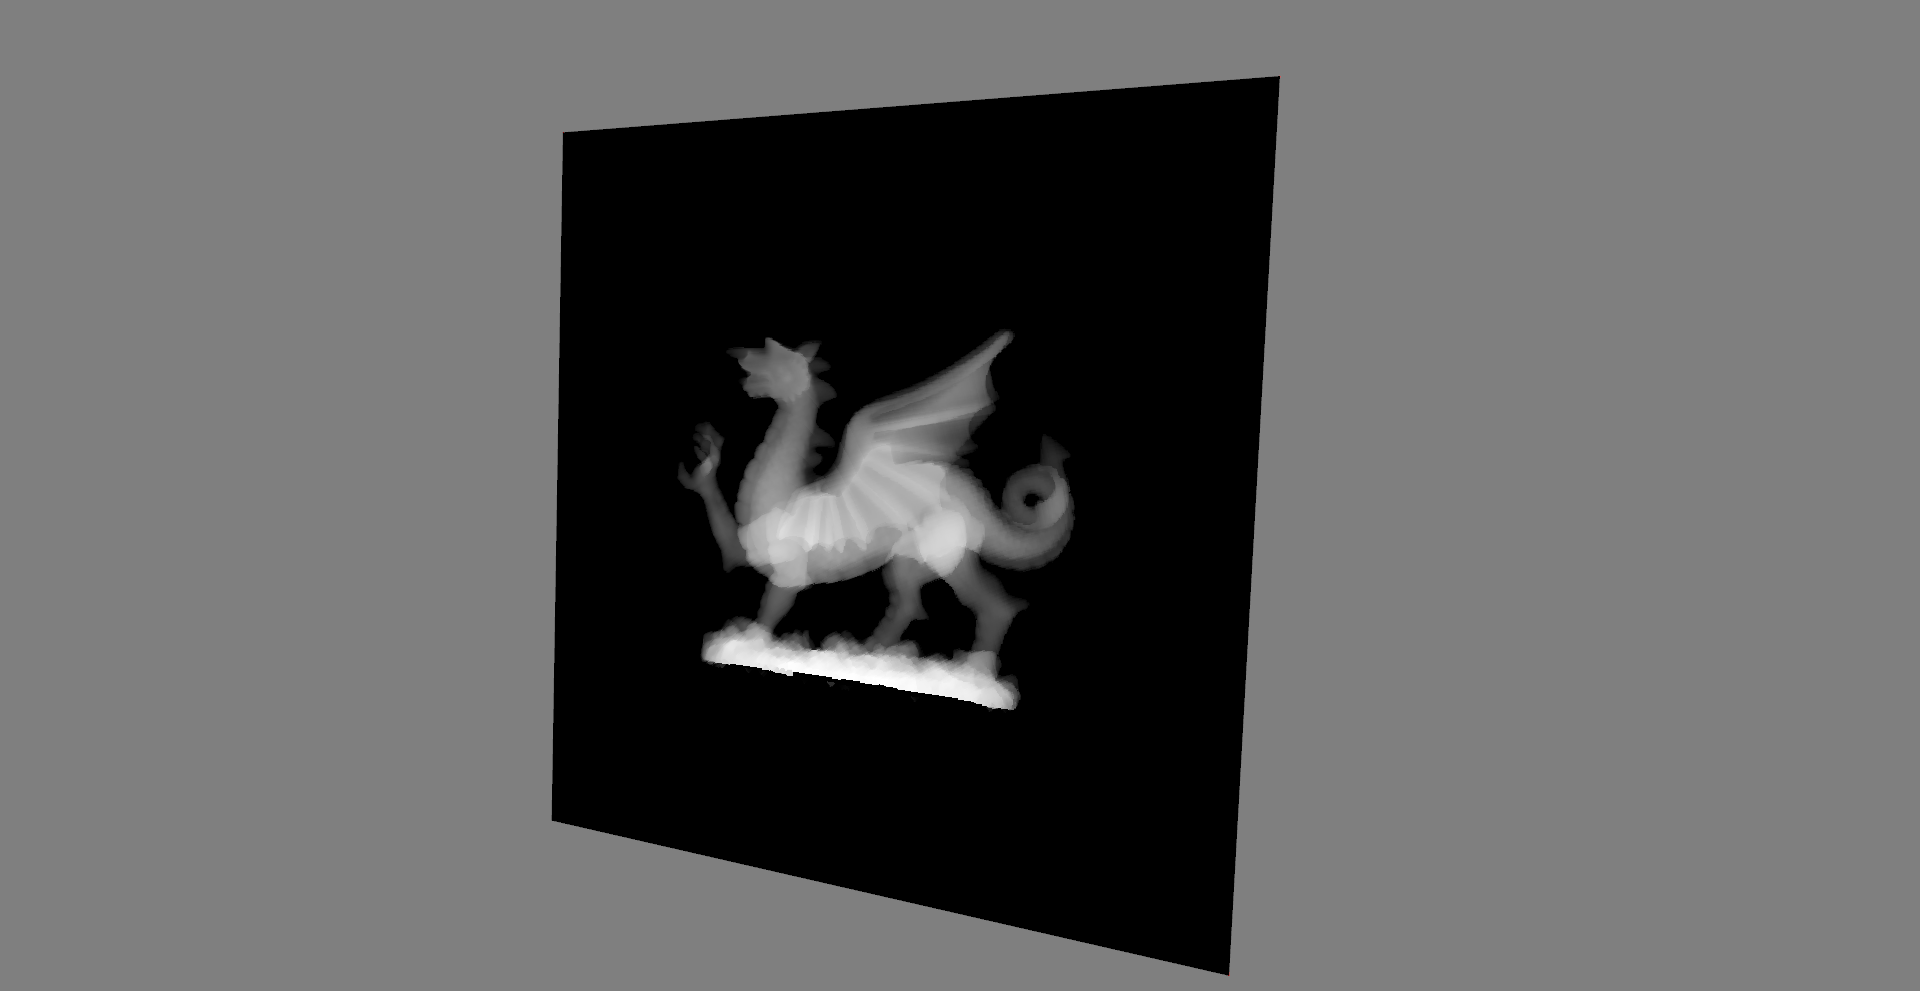
\includegraphics[width=0.25\textwidth]{point_source_xray.png}	&	(the image on the right-hand side is sharper) \\
		\hline
		    \multirow{2}{*}{Key: \texttt{4}}	&	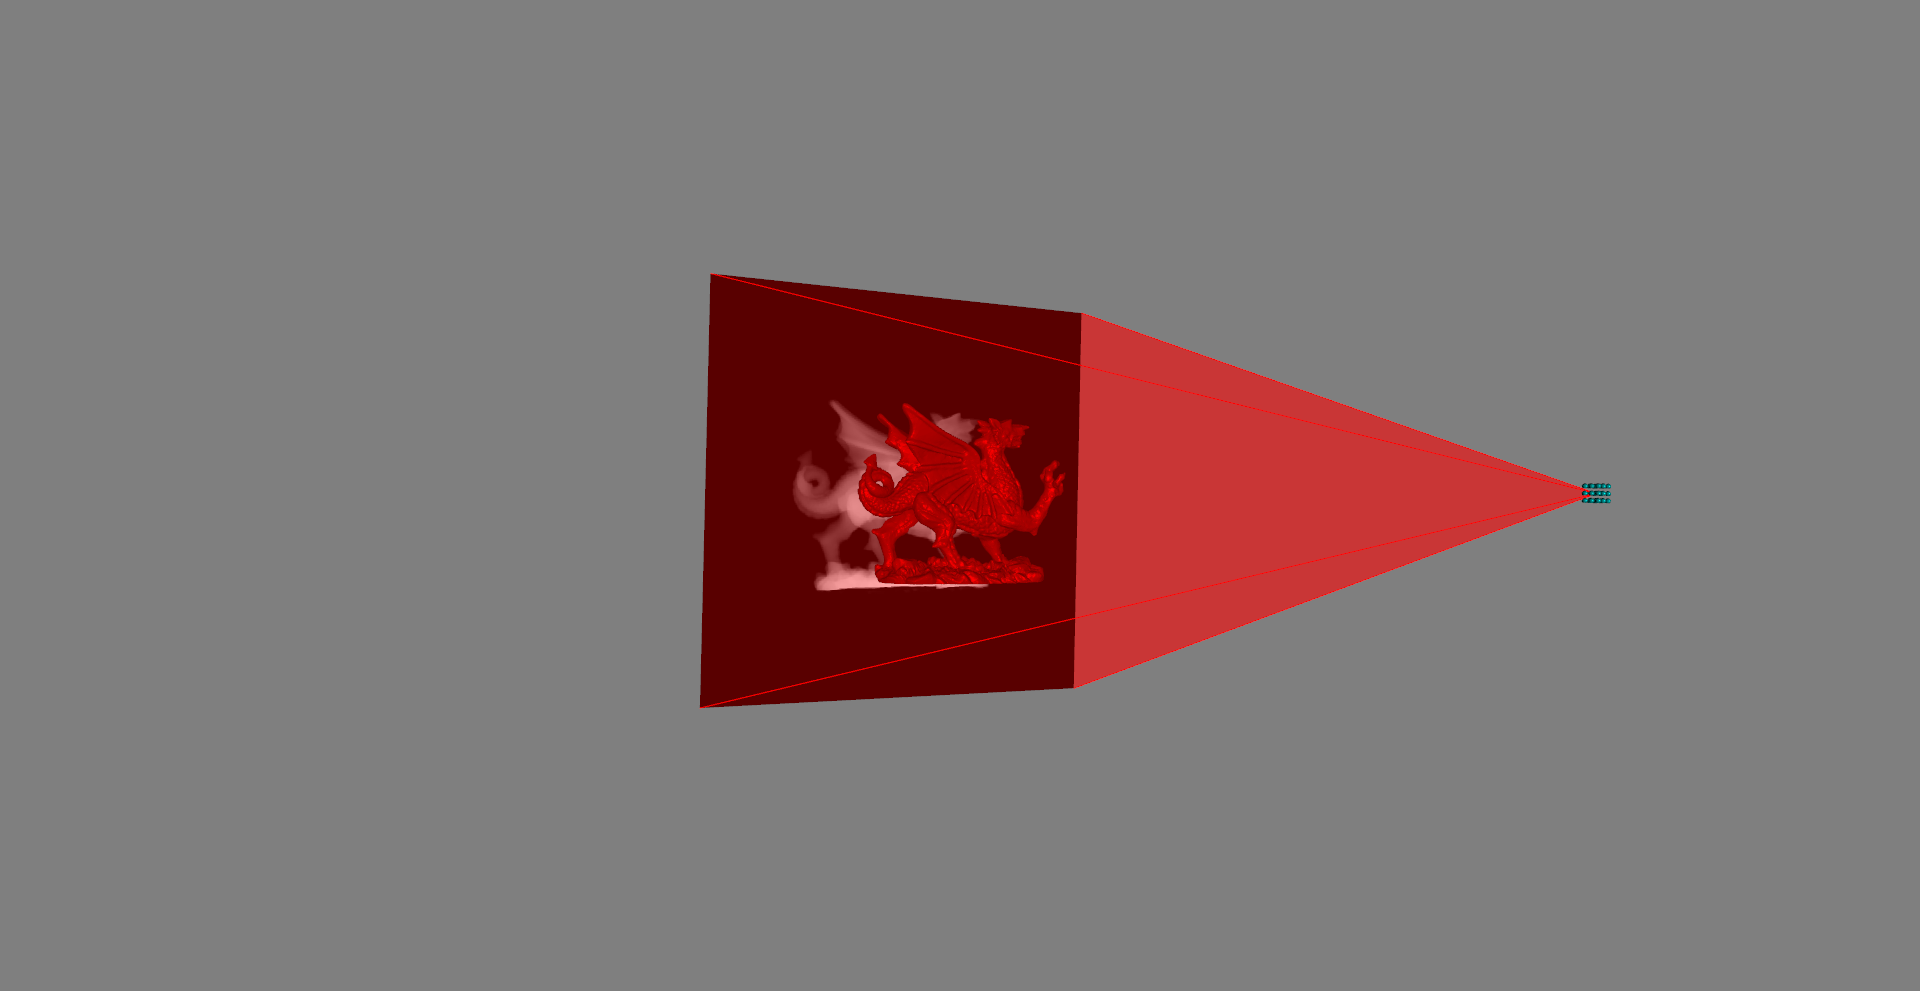
\includegraphics[width=0.25\textwidth]{cube_source.png}	&	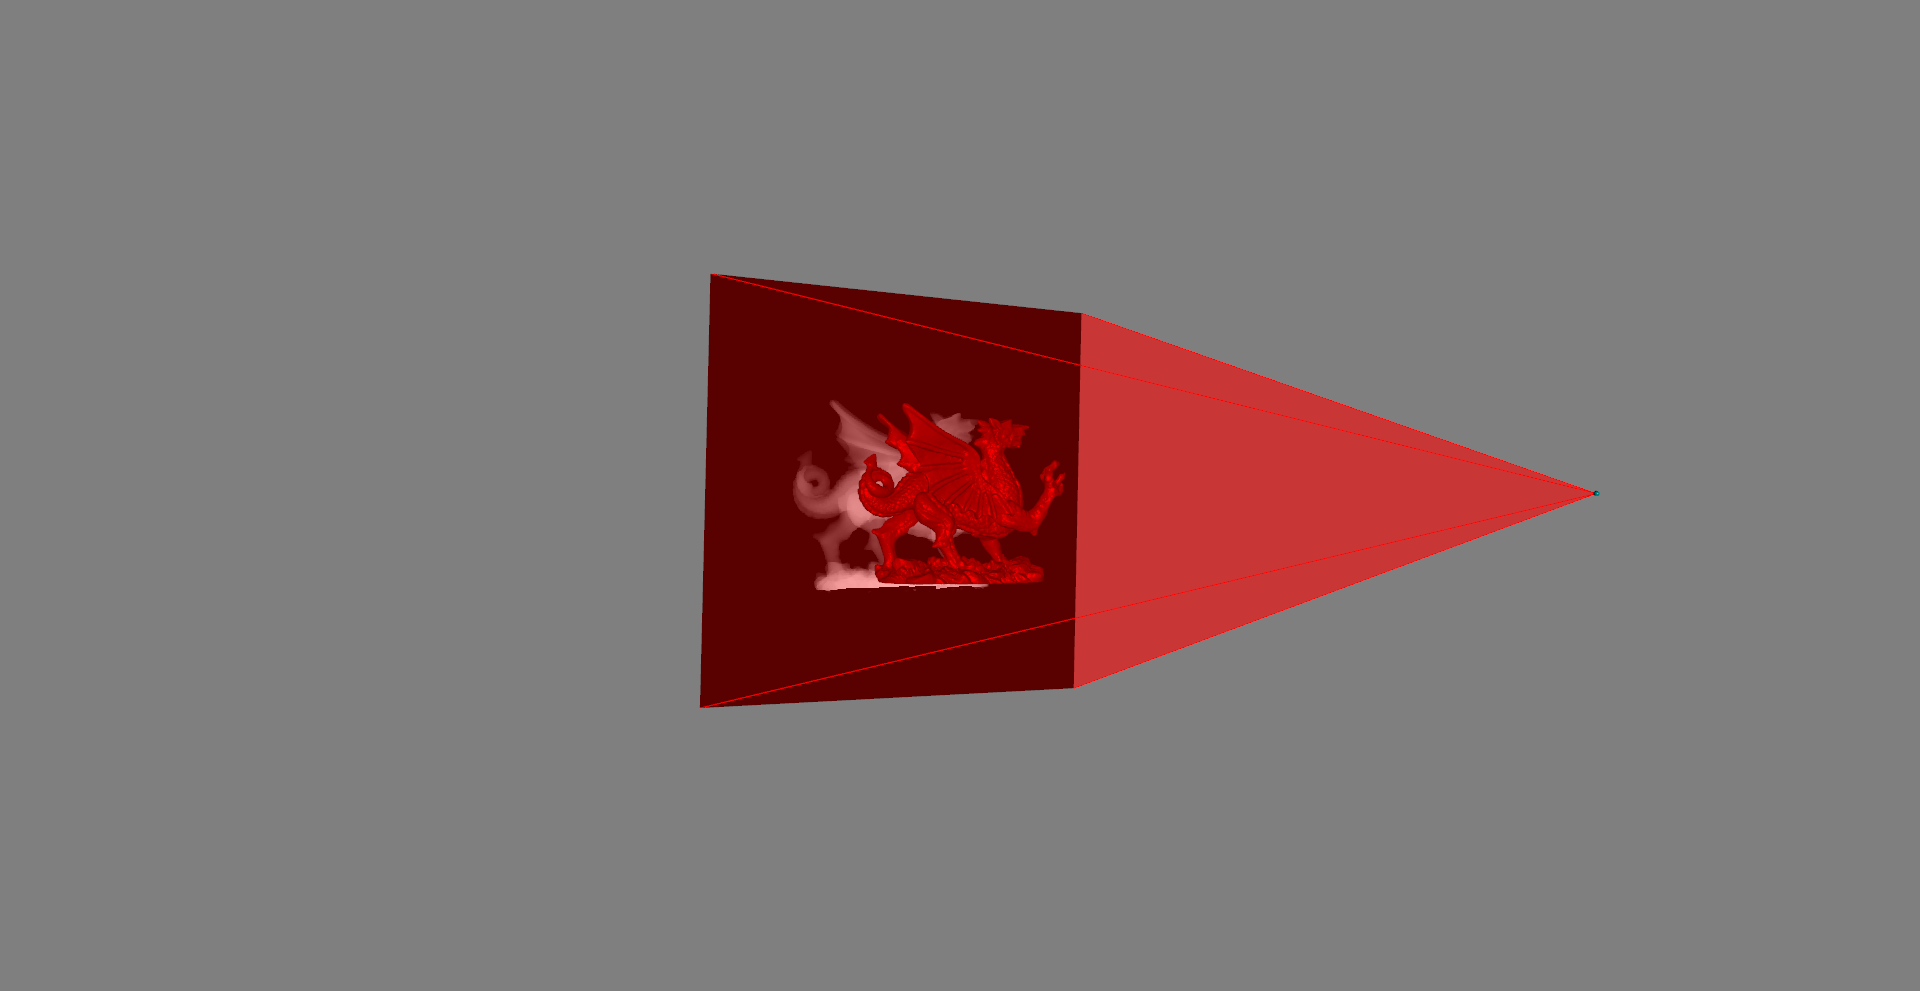
\includegraphics[width=0.25\textwidth]{point_source.png}	&	Use a cube source/Use a point source\\
			&	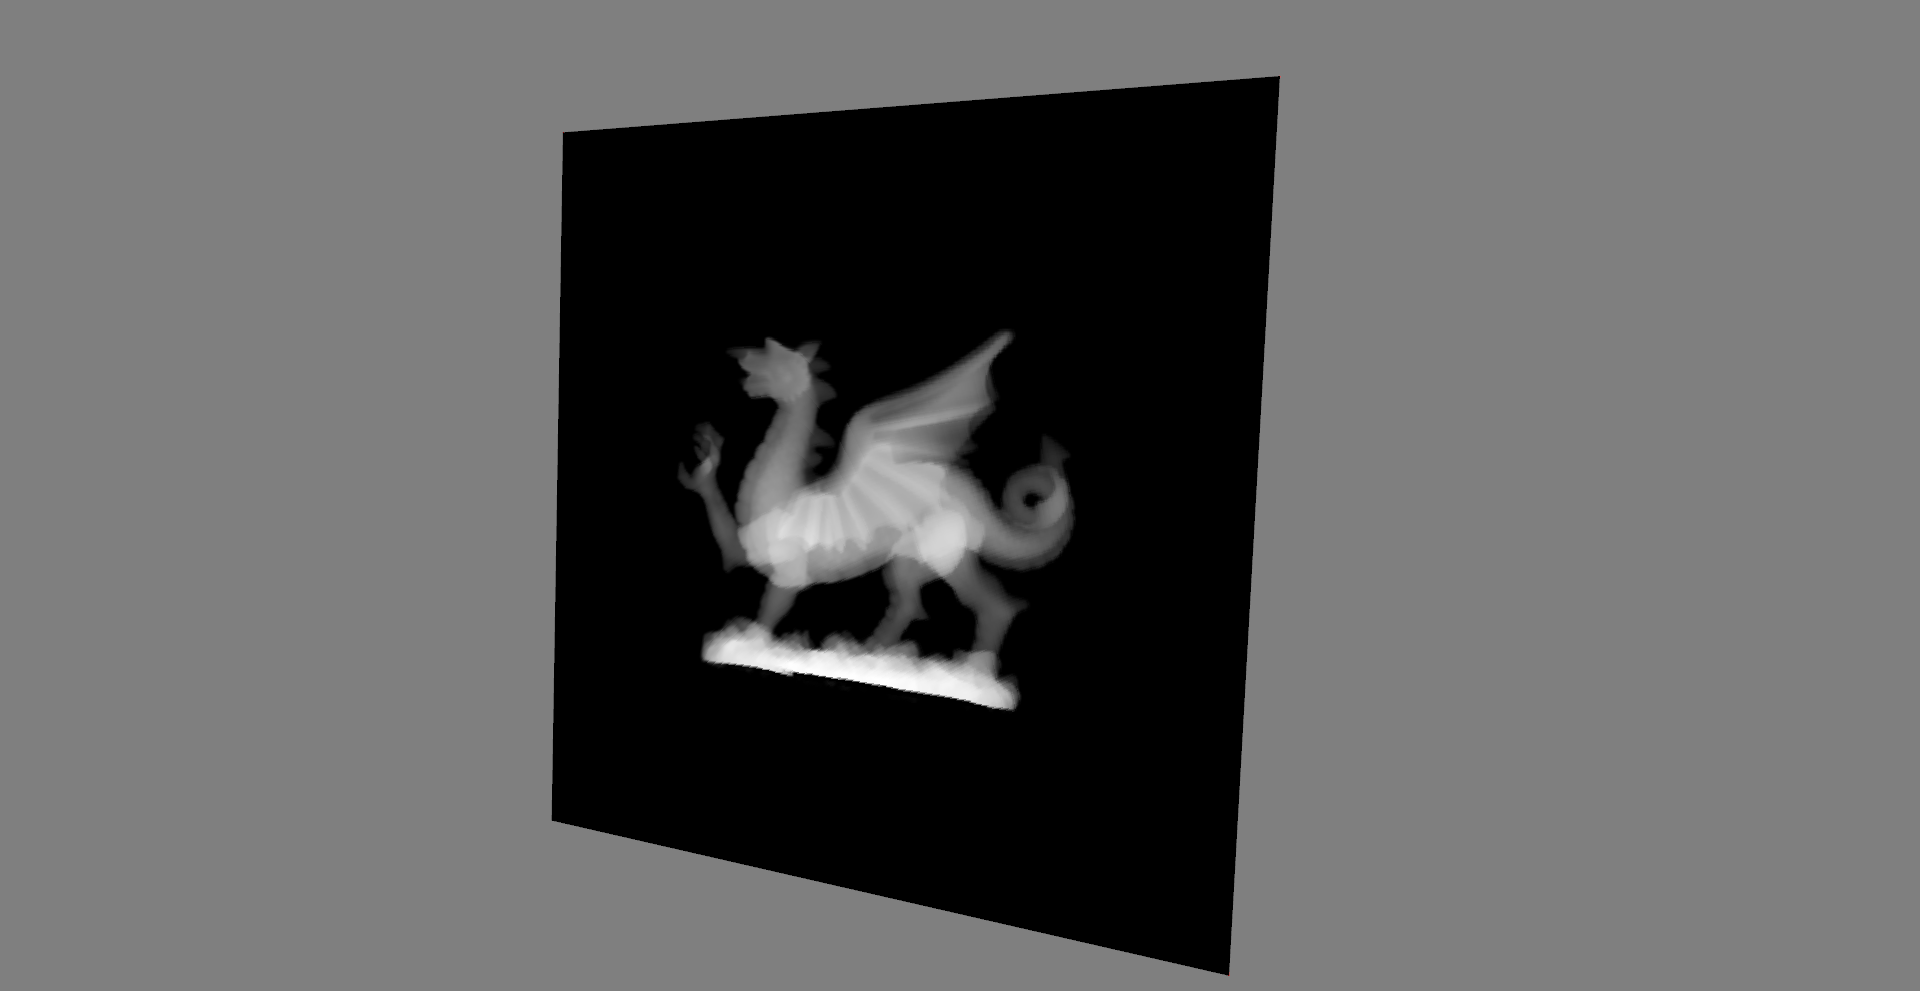
\includegraphics[width=0.25\textwidth]{cube_source_xray.png}	&	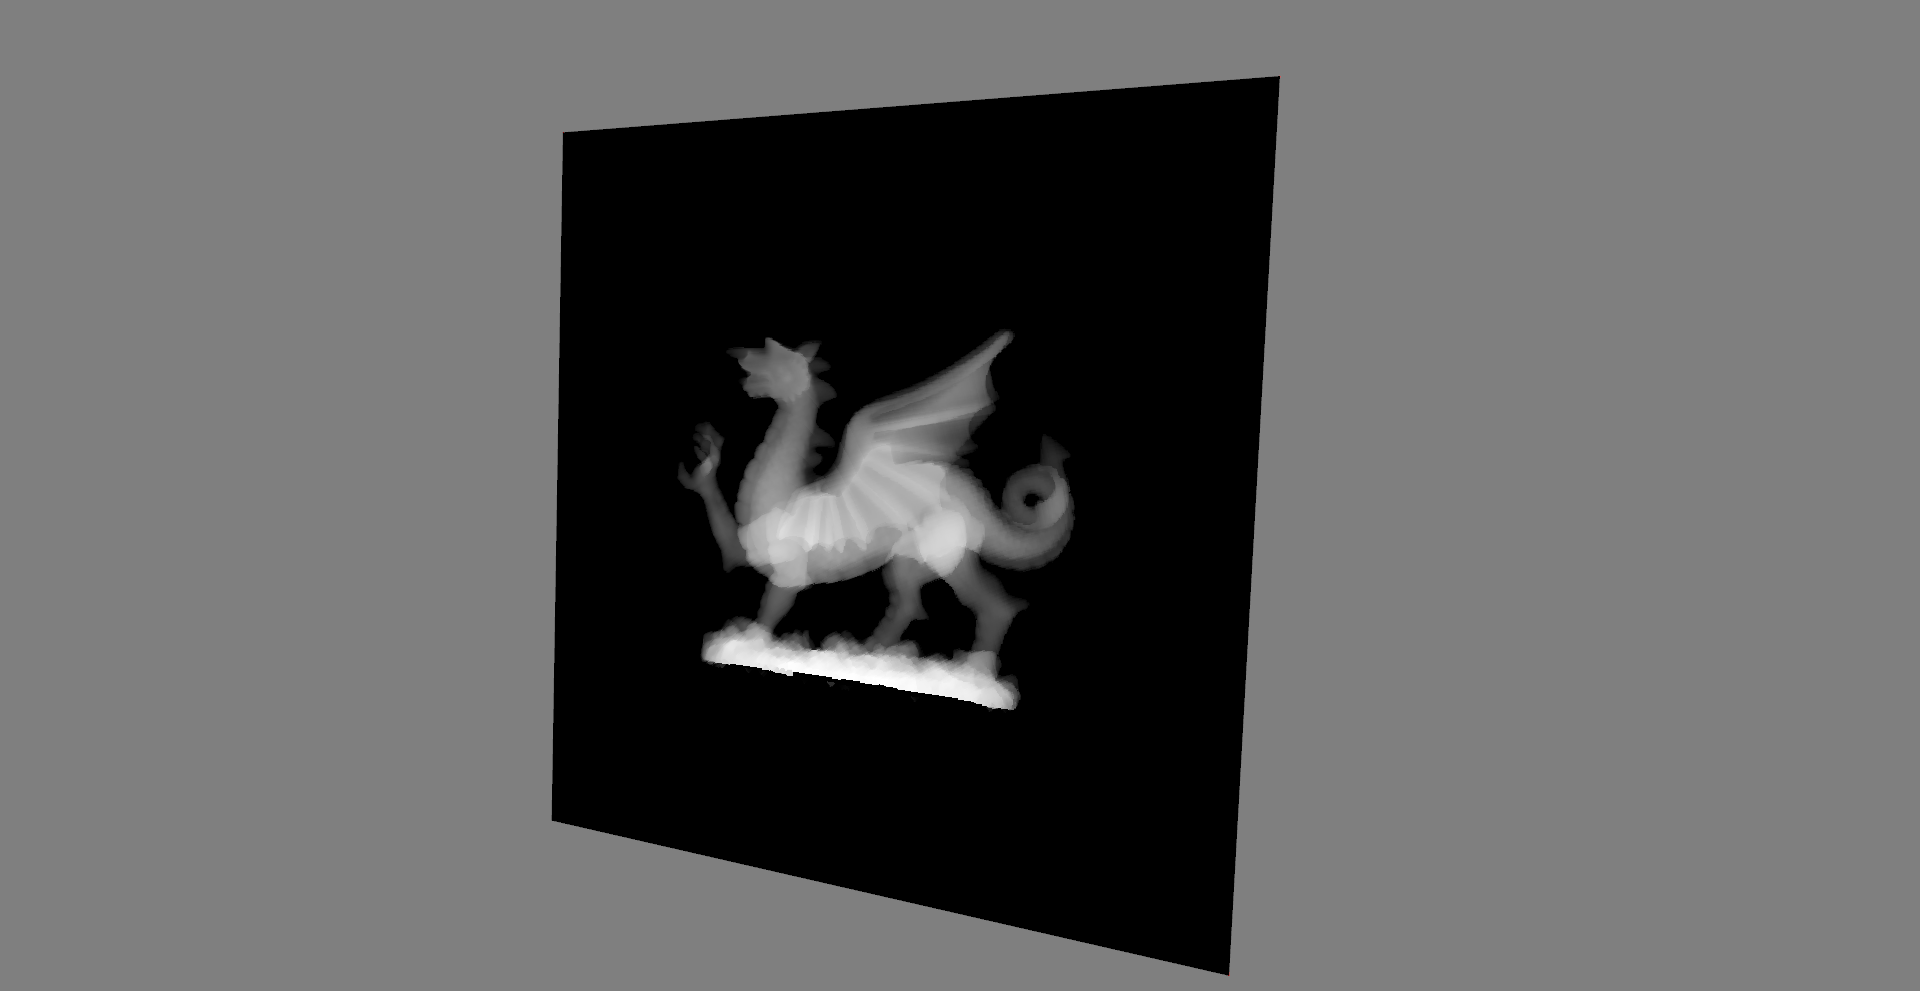
\includegraphics[width=0.25\textwidth]{point_source_xray.png}	&	(the image on the right-hand side is sharper) \\
% 		\hline
% 		Mouse wheel	&	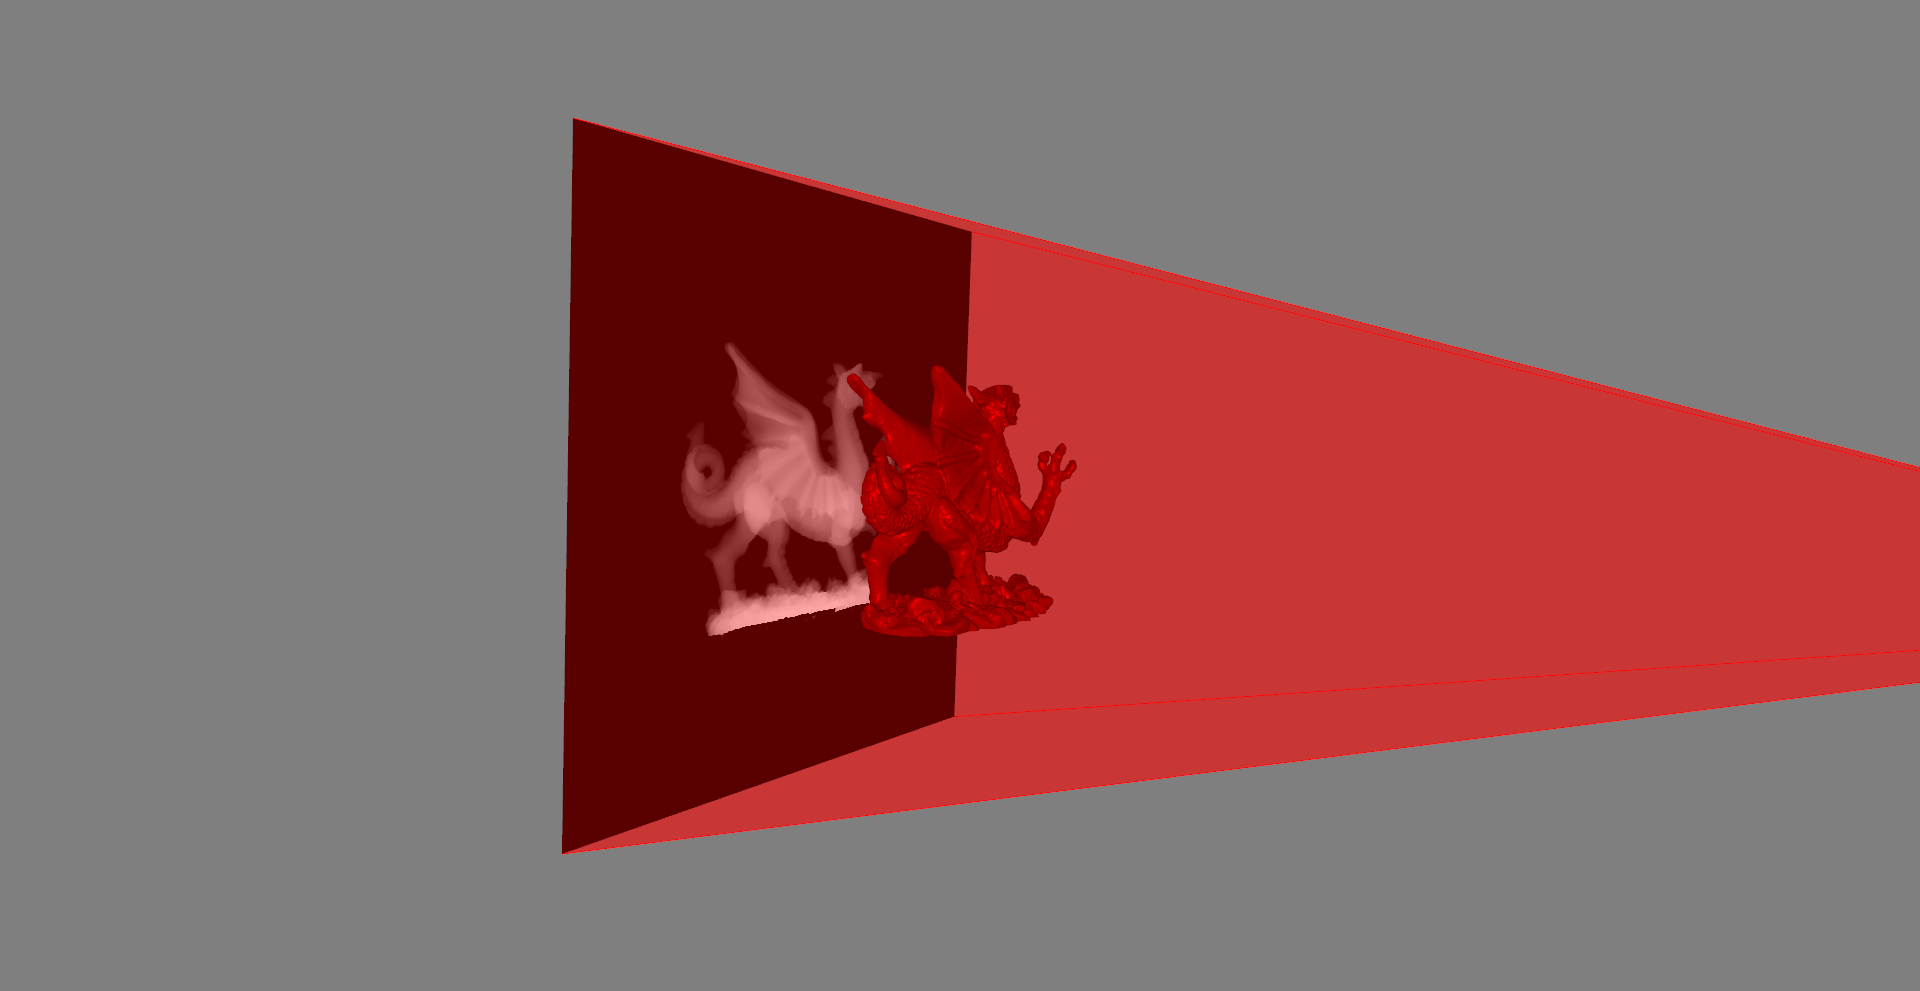
\includegraphics[width=0.25\textwidth]{mouse_wheel_zoom_in.png}	&	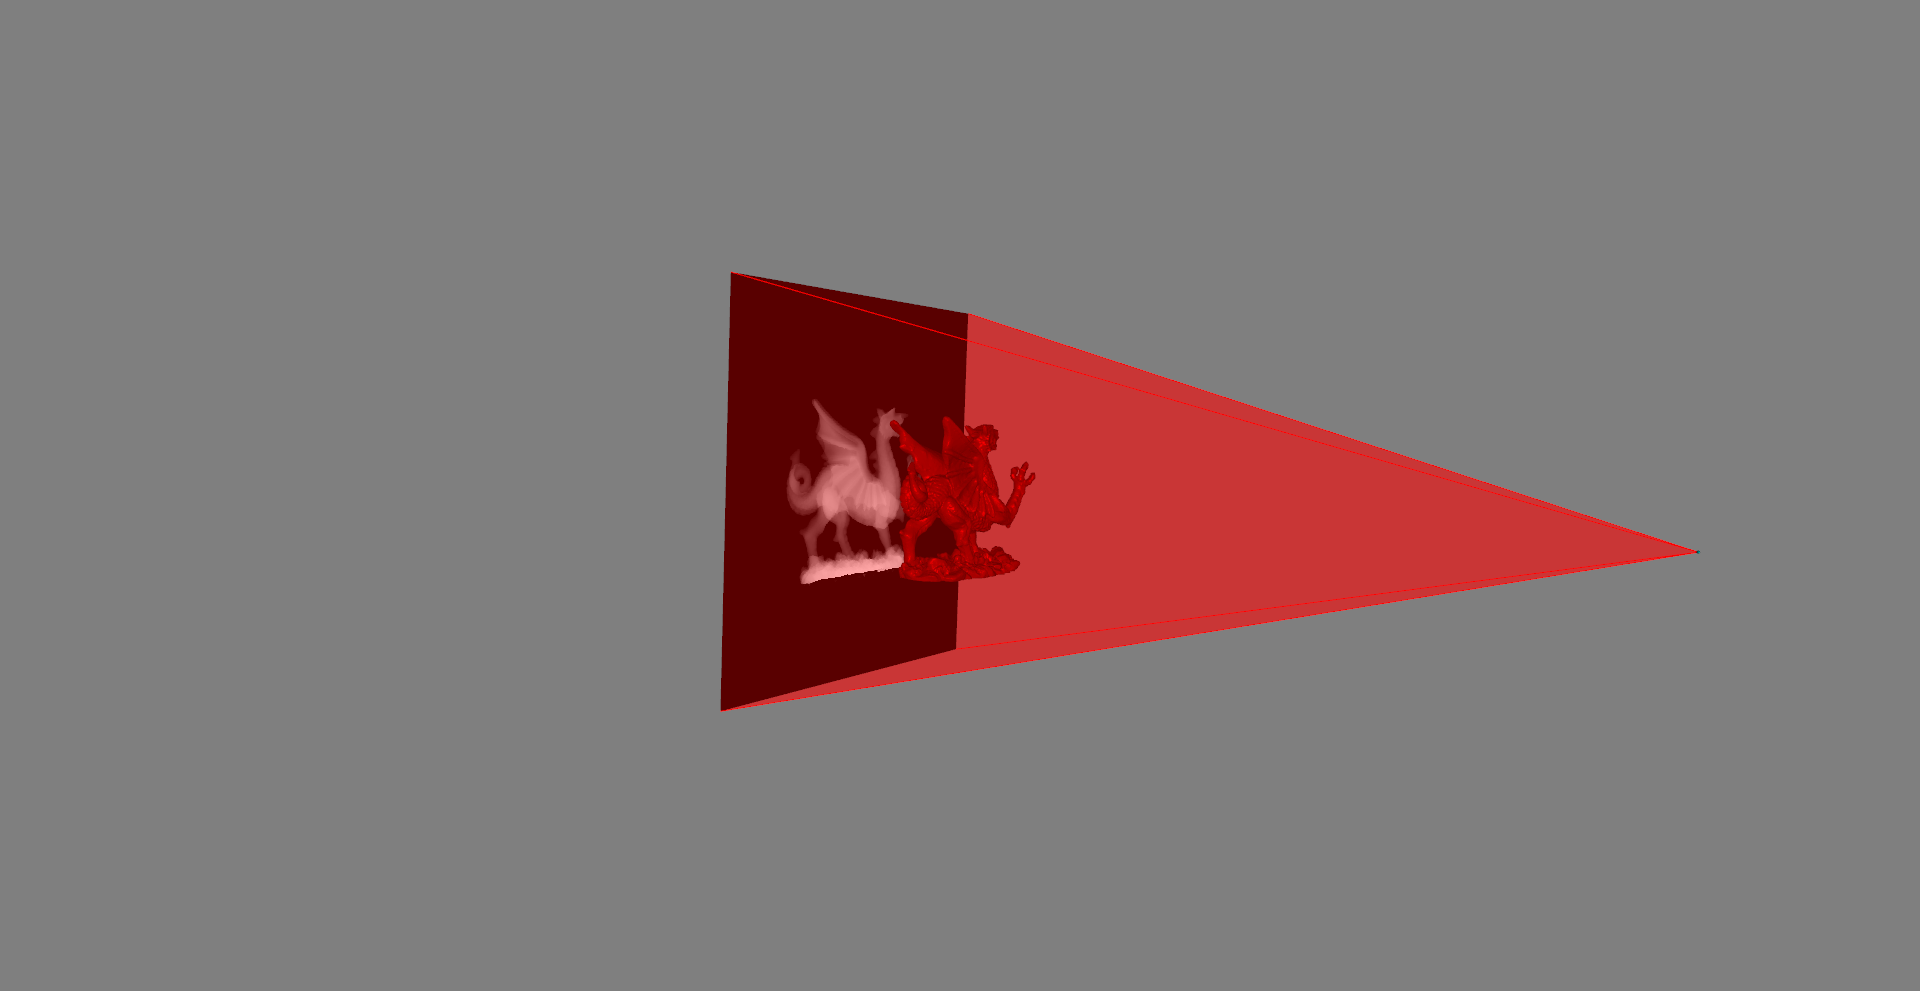
\includegraphics[width=0.25\textwidth]{mouse_wheel_zoom_out.png}	&	Zoom in/out\\
% 		\hline
% 		Mouse left button	&	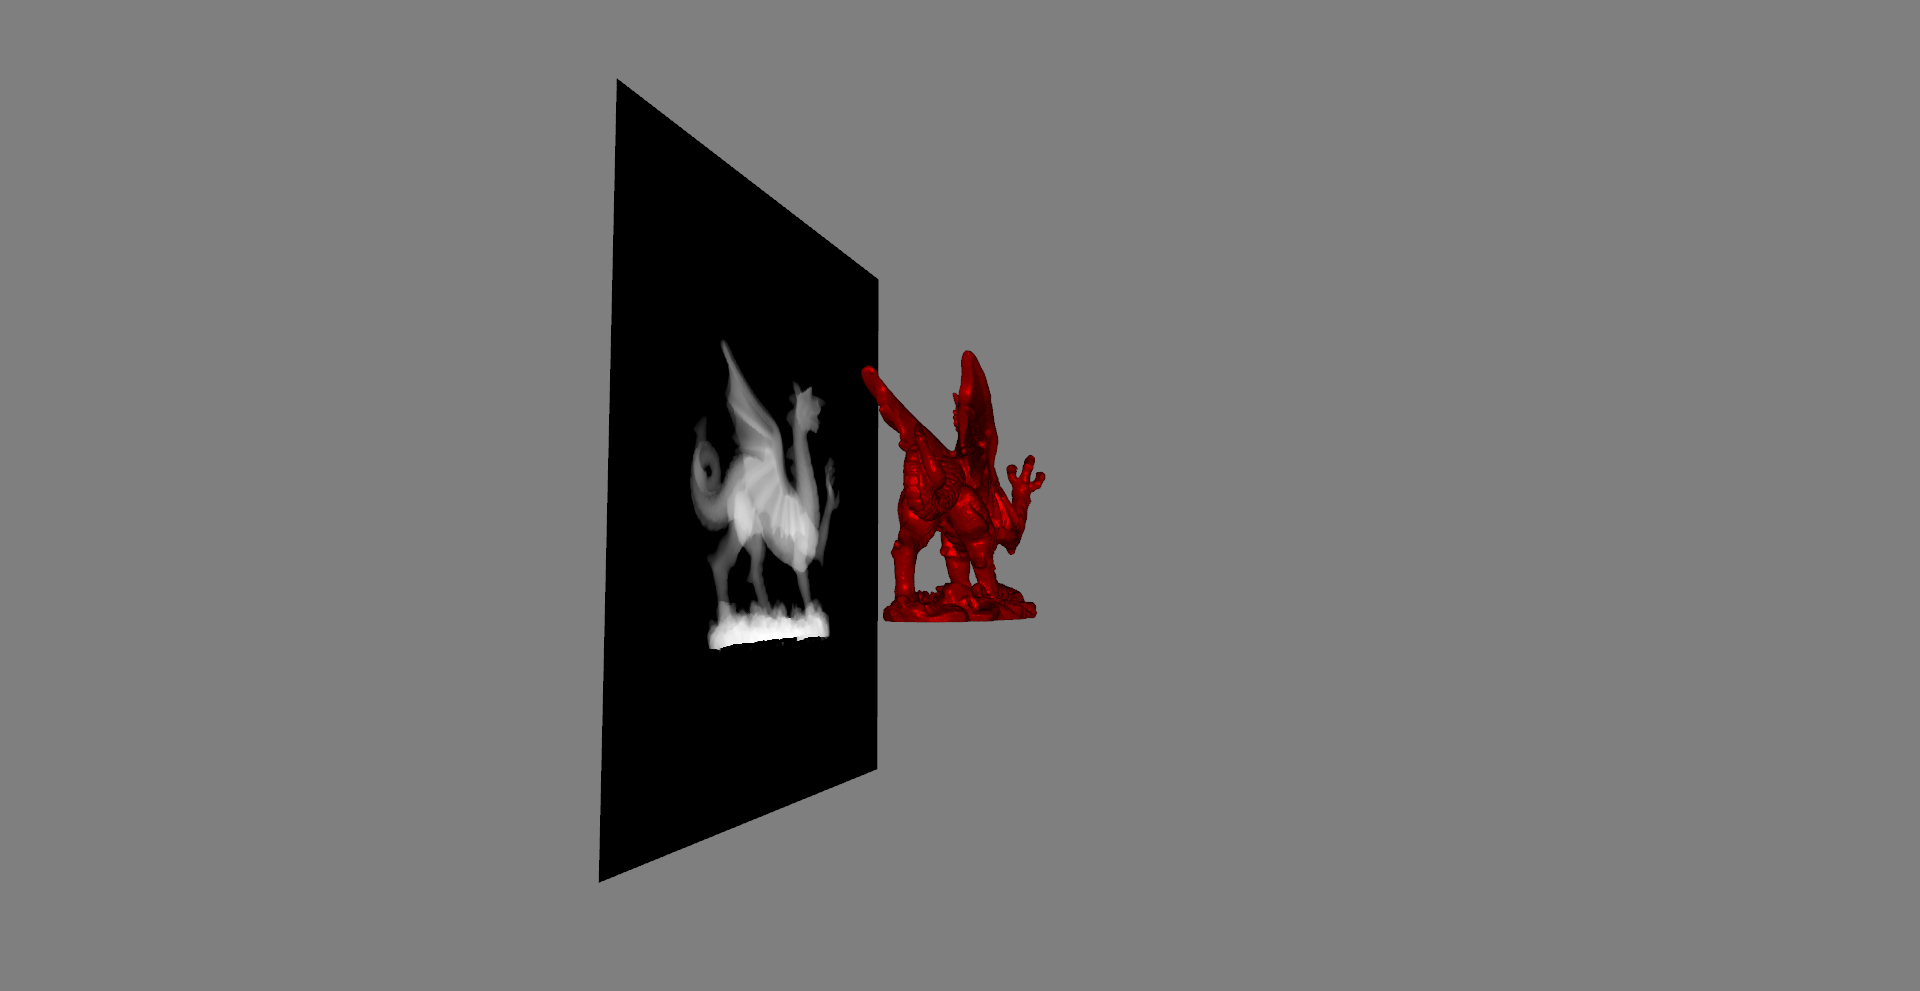
\includegraphics[width=0.25\textwidth]{mouse_click.png}	&	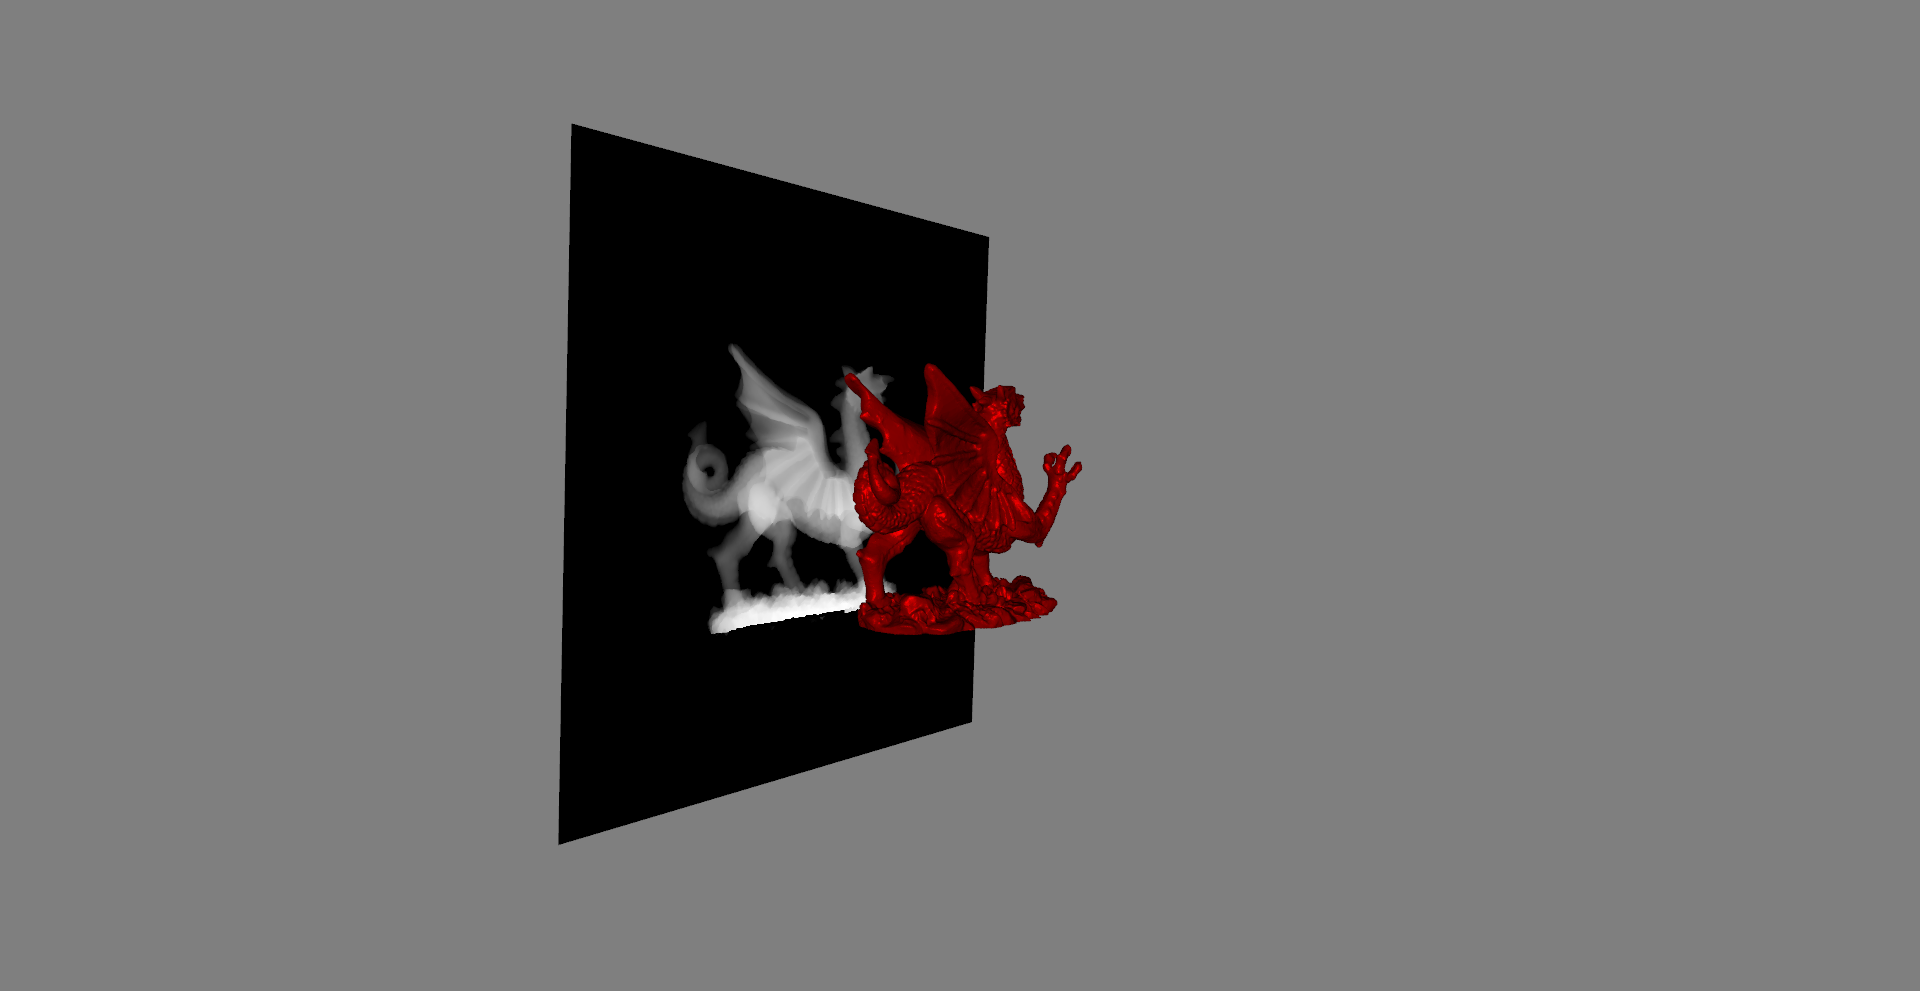
\includegraphics[width=0.25\textwidth]{mouse_left_click.png}	&	Rotate the virtual environment\\
% 		\hline
% 		Mouse middle button	&	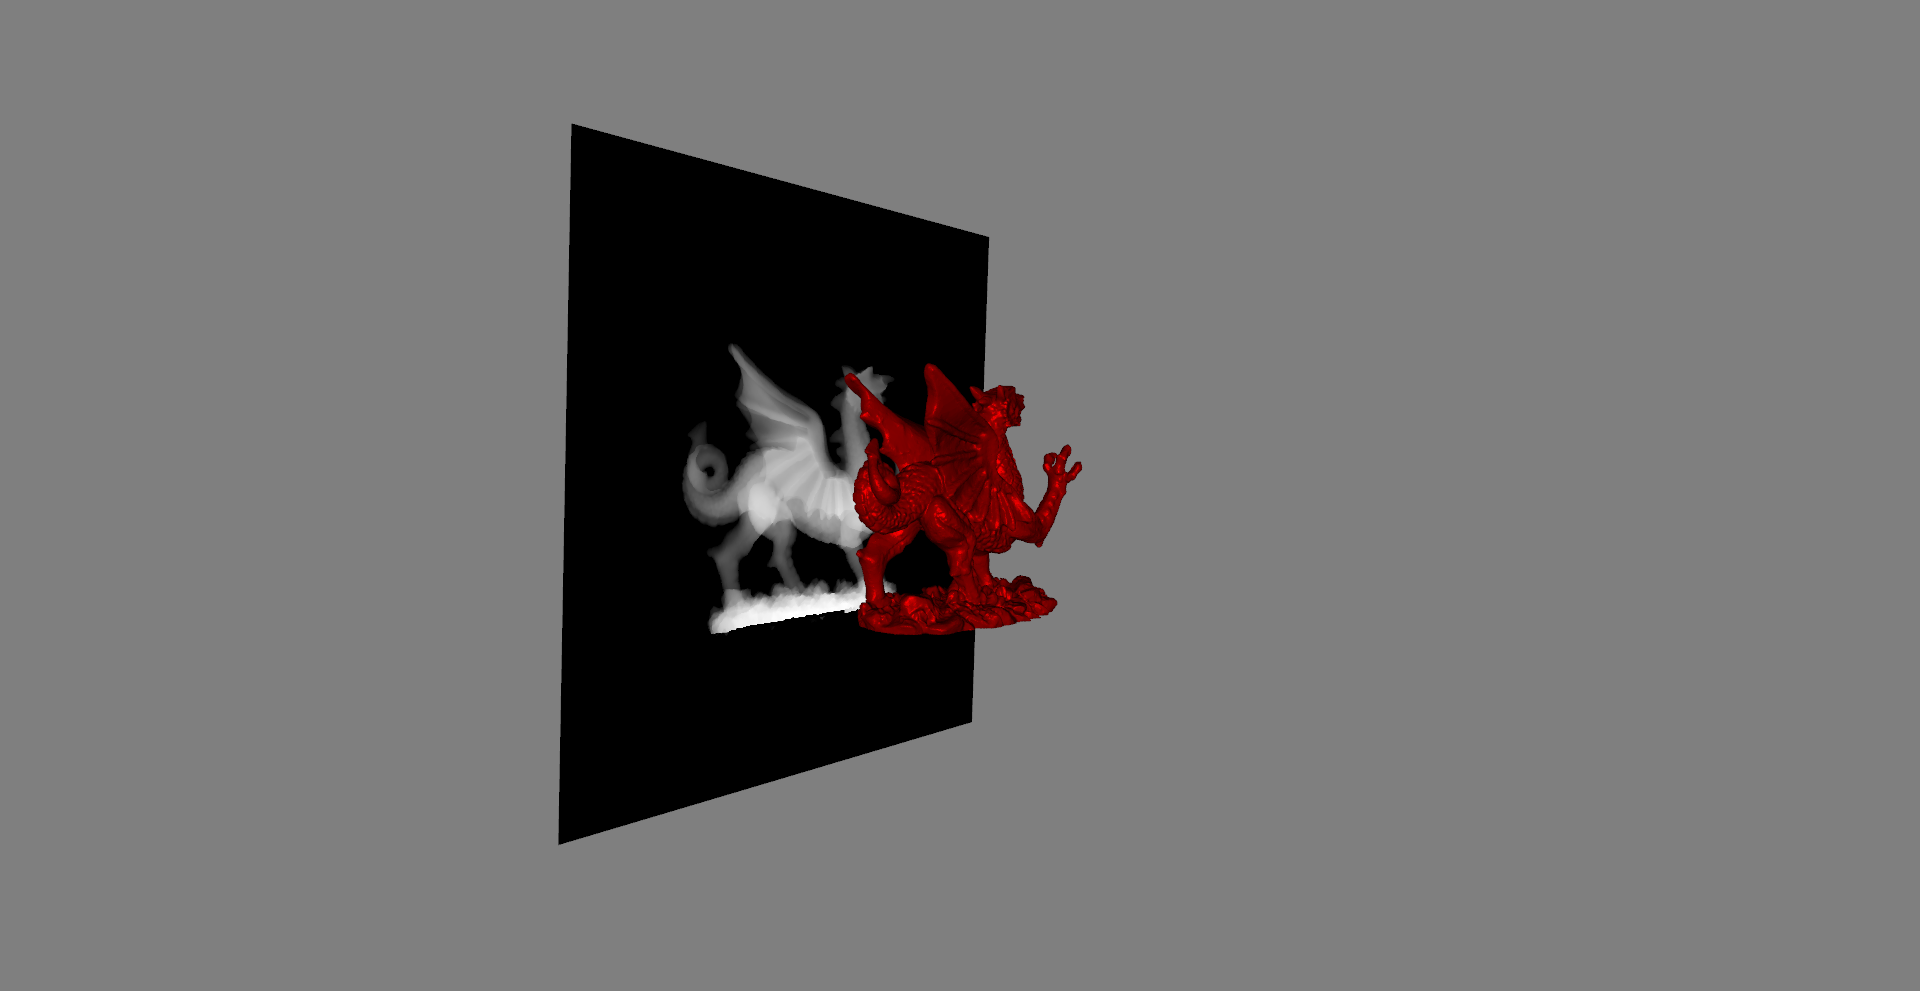
\includegraphics[width=0.25\textwidth]{mouse_left_click.png}	&	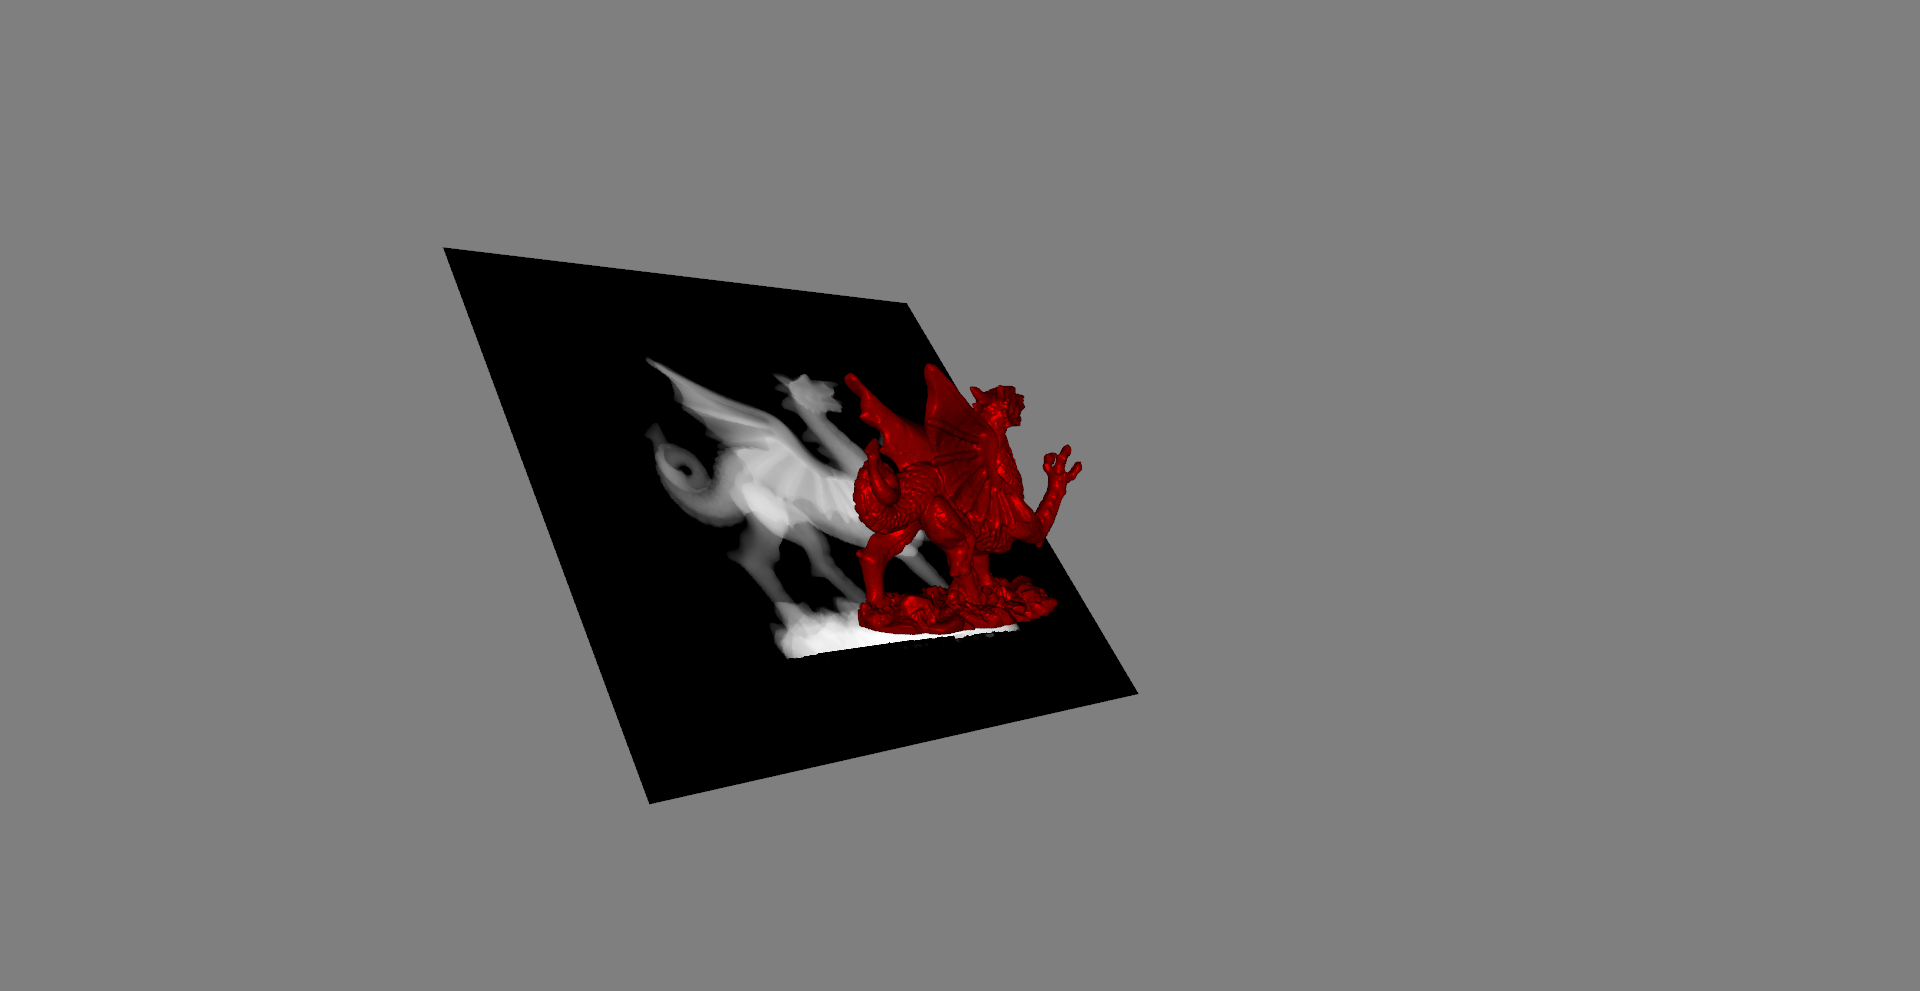
\includegraphics[width=0.25\textwidth]{mouse_middle_click.png}	&	Rotate the X-ray detector\\
% 		\hline
% 		Mouse right button	&	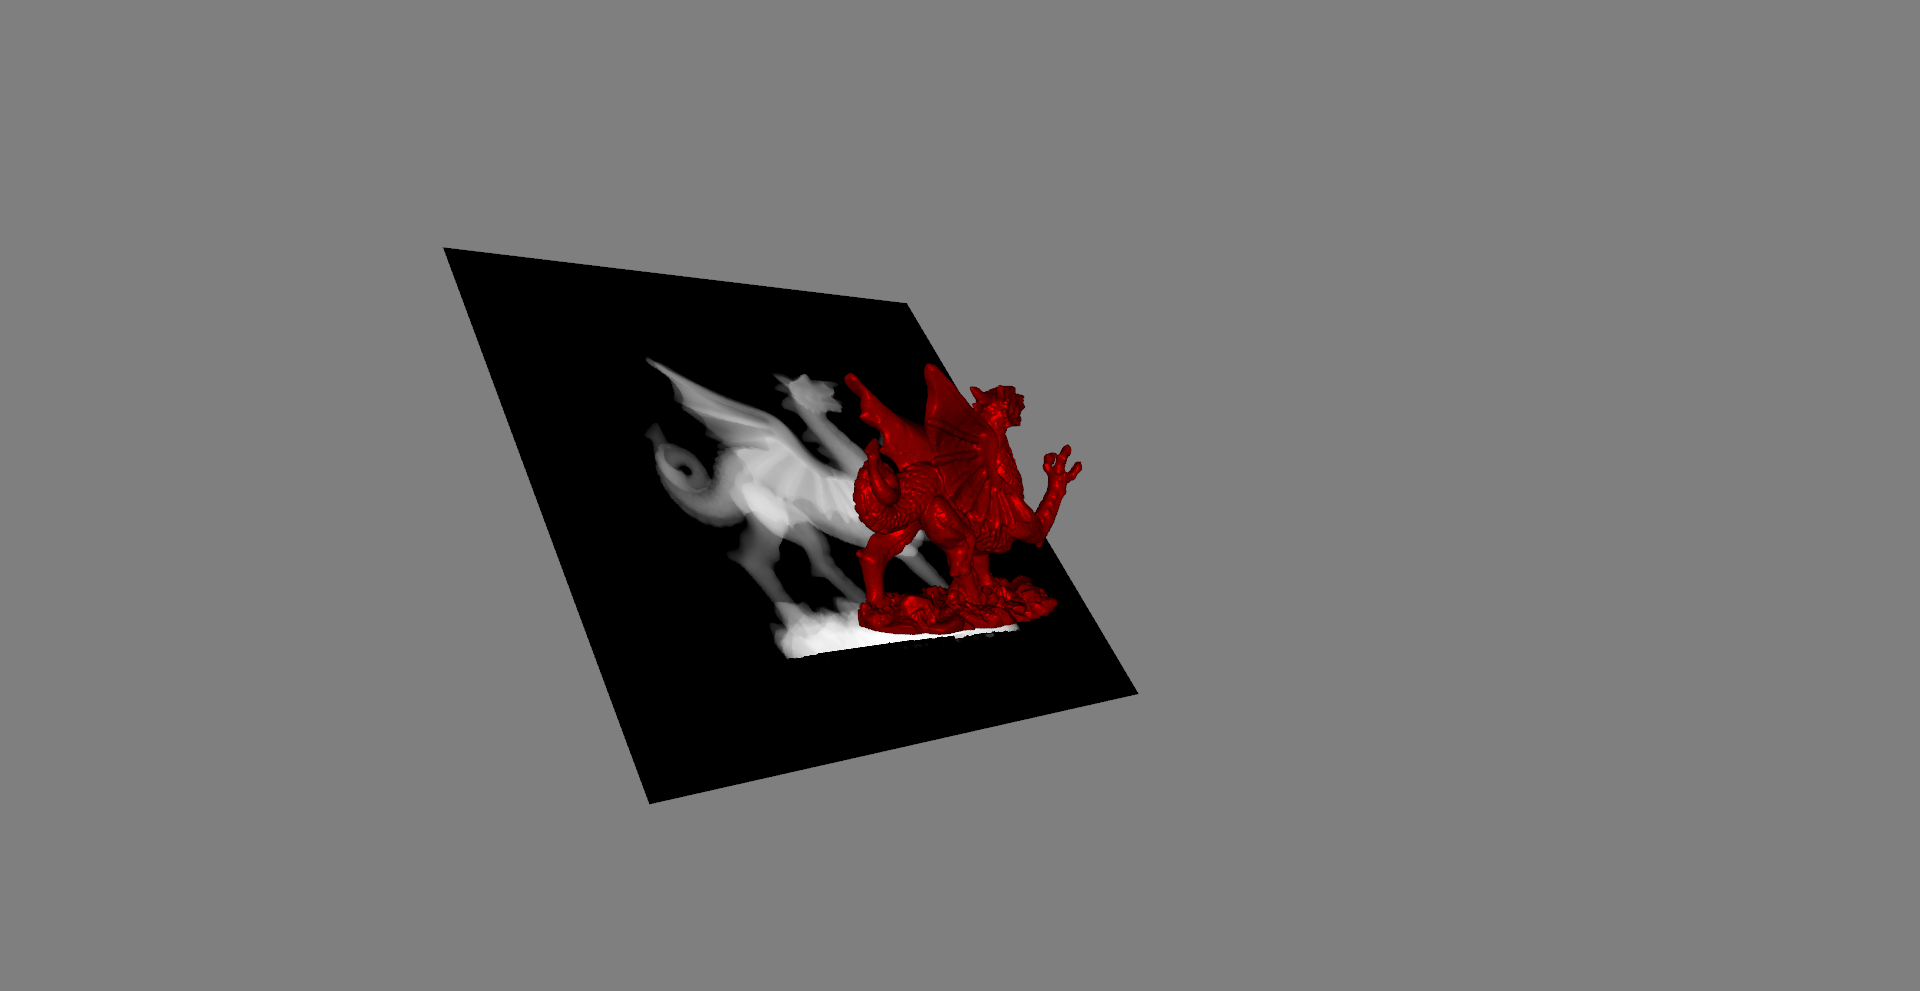
\includegraphics[width=0.25\textwidth]{mouse_middle_click.png}	&	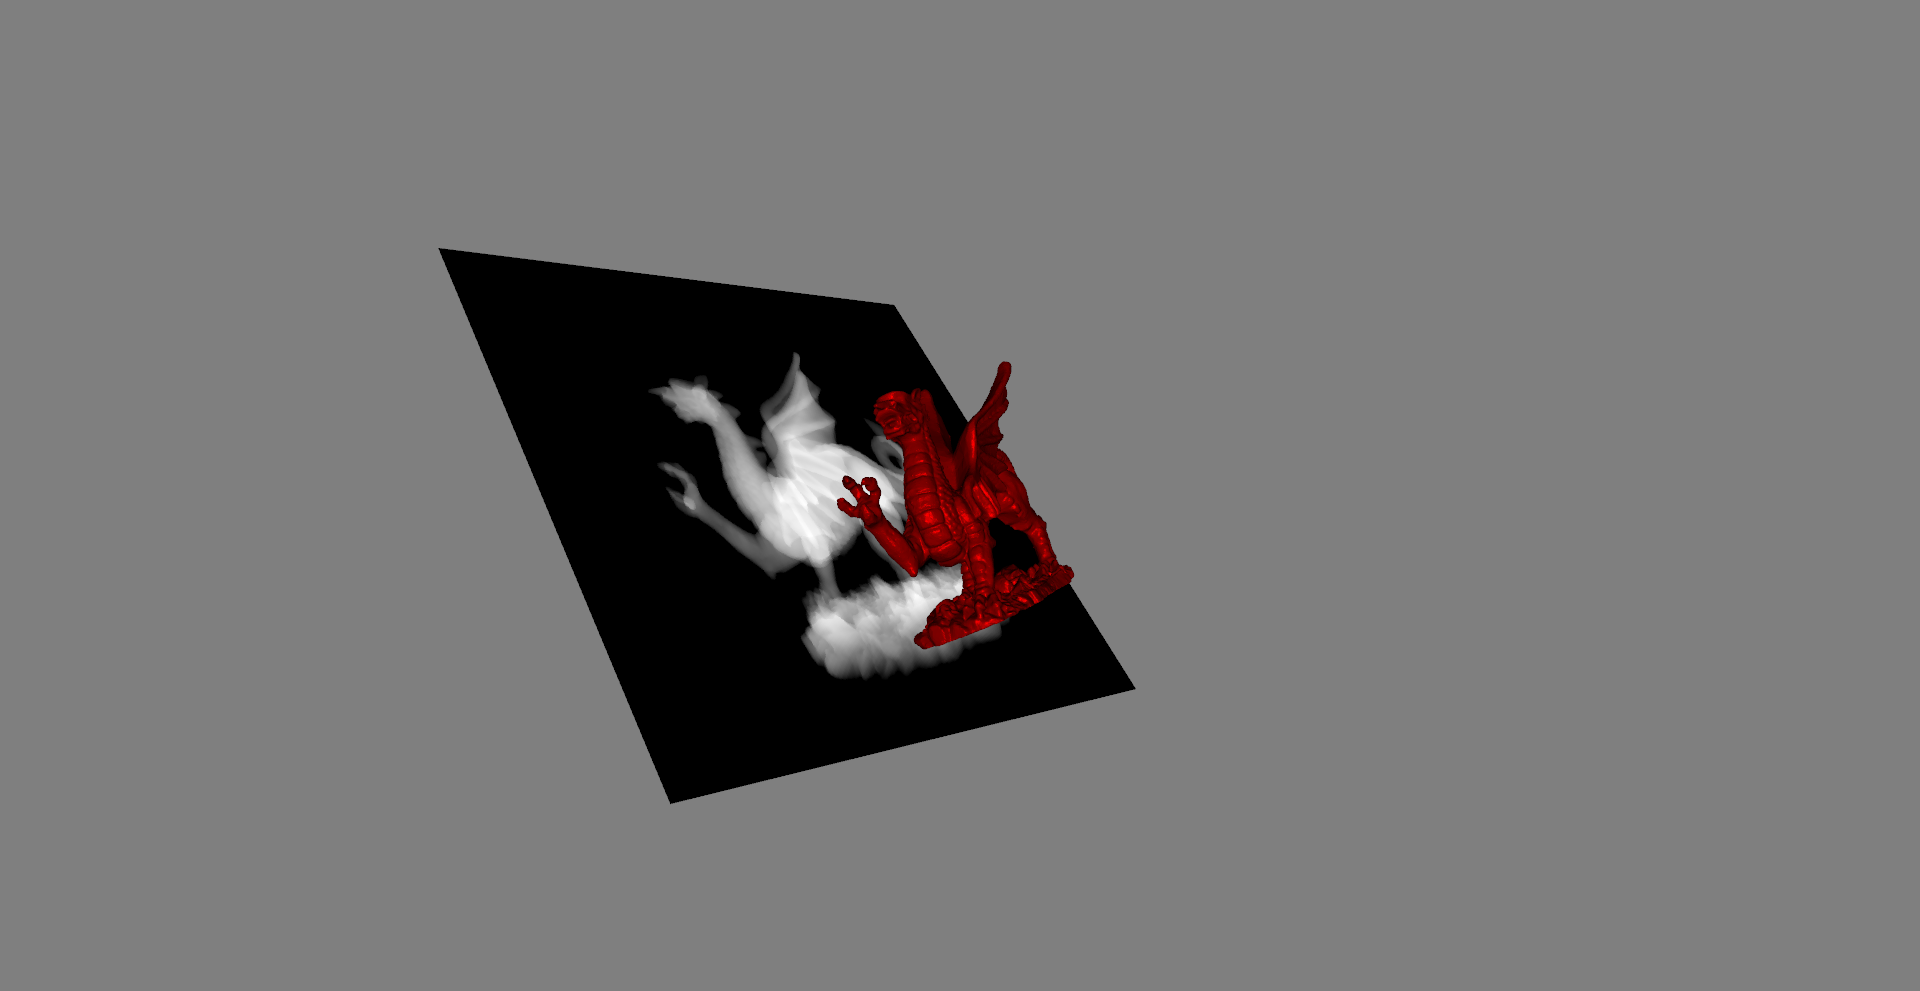
\includegraphics[width=0.25\textwidth]{mouse_right_click.png}	&	Rotate the dragon\\
		\hline
	\end{longtable}
\end{center}



% cube_source_xray.png
% line_source_xray.png
% .png
% .png
% .png
% point_source_xray.png
% square_source_xray.png

\end{document}
